% vim: tw=80:conceallevel=0
\documentclass[times, utf8, diplomski]{fer}
\usepackage{booktabs}
\usepackage{float}
\usepackage{graphicx}
\usepackage{pdfpages}
\usepackage{listings}

\begin{document}

\thesisnumber{2902}

\title{Razvoj informacijskog sustava za potporu organizaciji događanja s velikim
brojem sudionika korištenjem programskog okvira za ubrzani razvoj aplikacija}

\author{Fran Borčić}

\maketitle

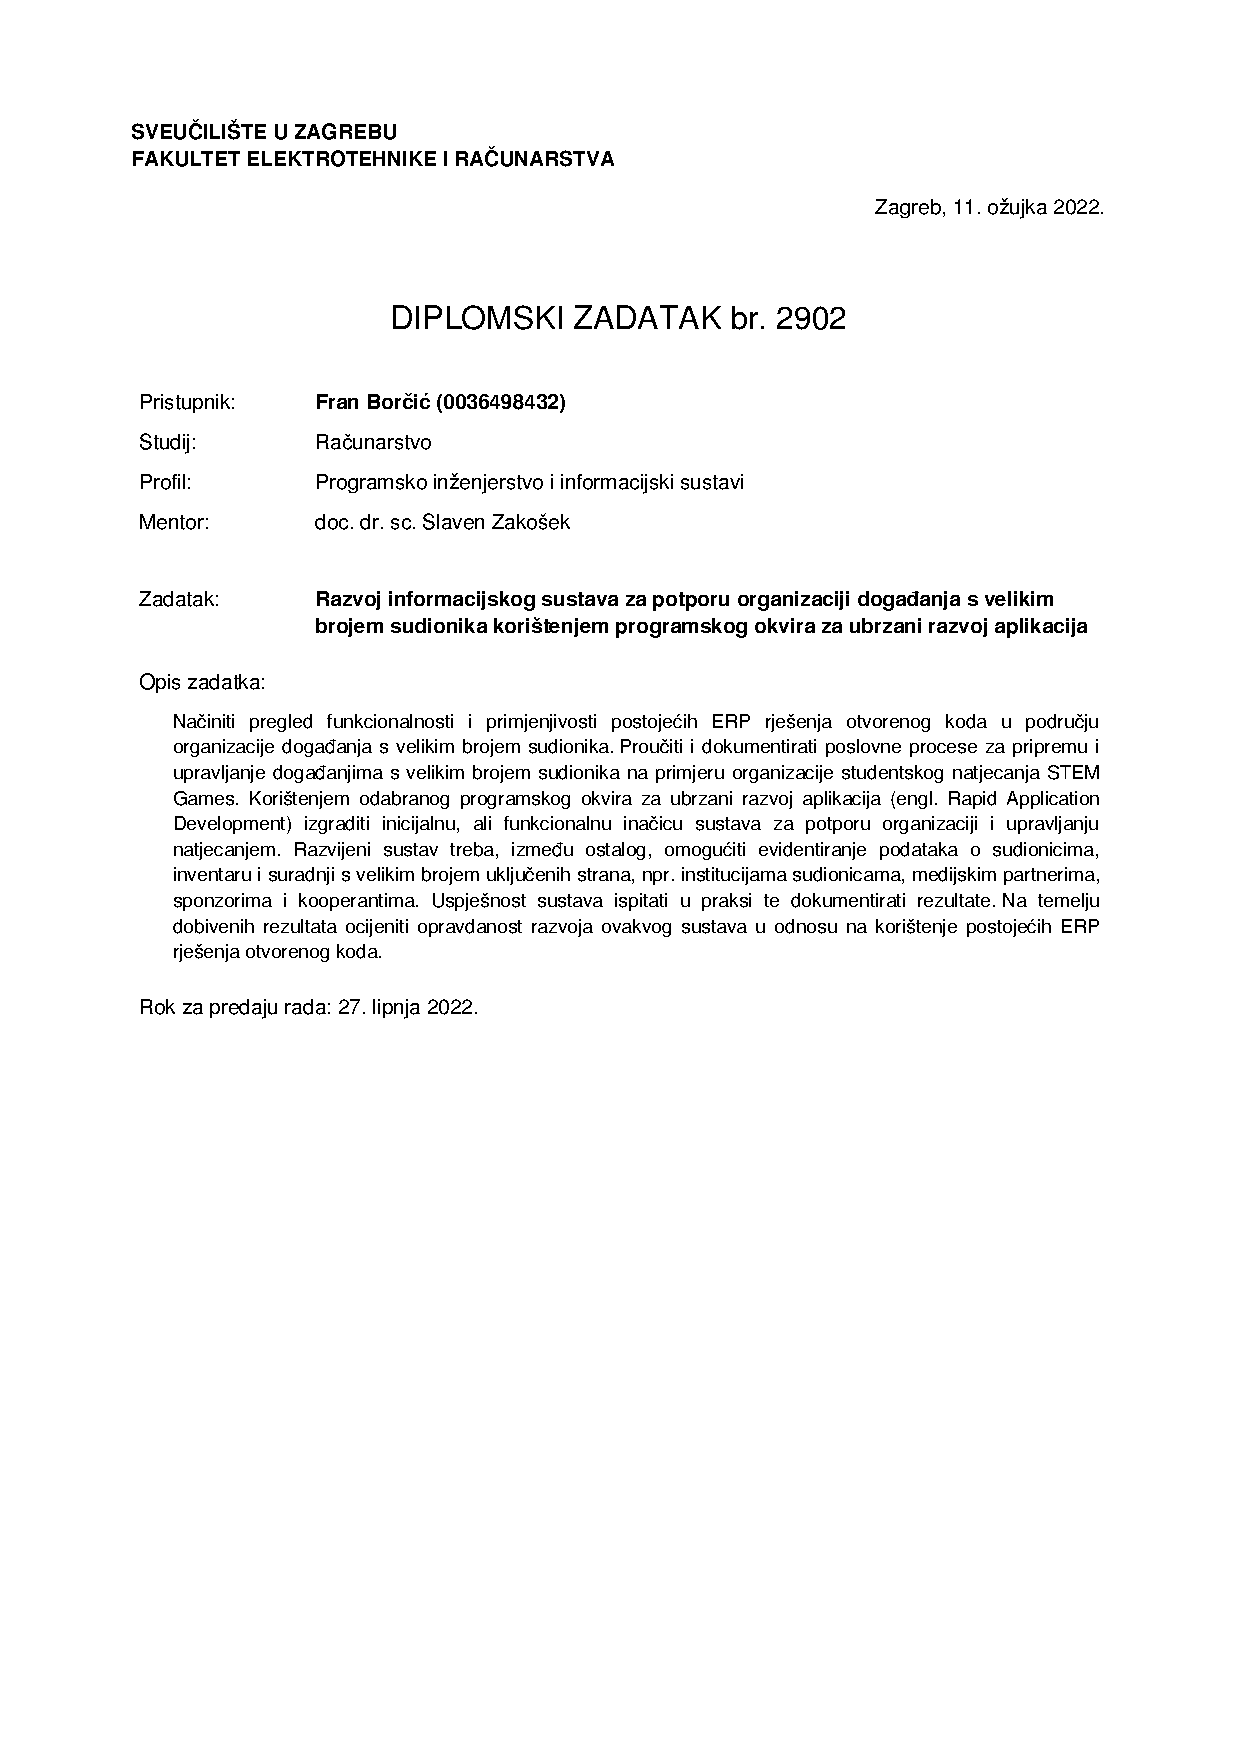
\includepdf{zadatak.pdf}

\zahvala{Zahvaljujem mentoru profesoru Slavenu Zakošeku na pomoći pri izradi
ovog rada.}

\tableofcontents

\chapter{Uvod}

Cilj ovog rada je ocijeniti mogućnost i isplativost implementacije
informacijskog sustava u rad studentskih organizacija koje se bave organizacijom
studentskih natjecanja s velikim brojem sudionika. Problemu će se pristupiti s
dva različita aspekta -- analizom prikladnosti postojećih rješenja i razvojem
osnovnog, ali primjenjivog prilagođenog rješenja koristeći programski okvir za
ubrzani razvoj aplikacija \engl{RAD}, a vodeći se konkretnim primjerom
\emph{Udruge za studentska natjecanja STEM Games}.

Tijekom posljednjih nekoliko desetljeća svjedočimo sve većoj prisutnosti
informacijskih sustava u poslovanju komercijalnih organizacija, većinom u vidu
radnih okvira poznatih kao \emph{ERP} sustavi. Pojam \emph{ERP rješenje}
\engl{enterprise resource planning} obuhvaća veliki broj informacijskih sustava
različitih vrsta i primjena, no prema definicijama navedenima u
(\cite{evolutionerp})
taj se pojam odnosi na sustave koje karakterizira modularnost te centralizirana
pohrana svih podataka vezanih uz poslovanje jedne organizacije.

Većina takvih sustava danas je realizirana kao skup gotovih modula oblikovanih
prema generičkim potrebama većeg broja komercijalnih organizacija
(\cite{bradford2014modern}). S obzirom na broj poslovnih procesa prisutnih u
svakoj takvoj organizaciji, takva arhitektura omogućuje ubrzanu implementaciju
većeg dijela informacijskog sustava i ponovnu uporabu novorazvijenih modula u
organizacijama sličnog područja rada.

Logična je posljedica spomenute arhitekture da je uvođenje ERP sustava u
poslovanje to jeftinije i jednostavnije što je više poslovnih procesa organizacije
u koju se uvodi prisutno i u drugim organizacijama. Organizacije koje se bave
rijetkim i specifičnim zadacima ograničene su u broju dostupnih rješenja kojima
mogu digitalizirati svoje poslovanje pa je slijedom toga i isplativost njihove
informatizacije znatno manja.

Slučaj koji će u ovom radu biti proučen, osim zbog svojih poslovnih procesa,
specifičan je i prema svojim ciljevima -- organizacija studentskih natjecanja na
području RH tradicionalno je neprofitnog karaktera, a iza takvih događaja stoje
studentske udruge ili udruge građana čiji su članovi volonteri. Iz tog razloga,
potencijalni benefiti uvođenja informacijskog sustava u tom području očitovali
bi se prije svega u jednostavnosti obavljanja volonterskog rada, a u znatno
manjoj mjeri kroz financijske pokazatelje. Također, takve organizacije uglavnom
ne mogu u svojim budžetima opravdati profesionalnu izradu informacijskog
sustava, ali su im dostupni ljudski resursi u obliku studenata volontera.

Eventualni informacijski sustavi koji bi bili prikladni za takve organizacije,
bili bi osmišljeni tako da se studenti volonteri uz minimalnu edukaciju mogu
brinuti o uvođenju i održavanju takvih sustava. S obzirom na sličnosti u formatu
različitih studentskih natjecanja na području RH, kroz ovaj rad nastojat će se
pronaći rješenje koje bi olakšalo organizaciju svih takvih događanja, a čija
primjena bi zahtijevala što manje tehničkog znanja.

Takvo što moglo bi se postići primjenom ERP rješenja otvorenog koda i prethodnom
pripremom njihove konfiguracije za konkretni zadatak organizacije. ERP rješenja
otvorenog koda za neprofitne organizacije postoje te će biti razmotrena u
nastavku rada, no s obzirom na činjenicu da se u ovom slučaju radi o vrlo
specifičnom tipu neprofitne organizacije takva rješenja ne mogu pokriti sve
njene potrebe.

Bolje prilagođeno rješenje, ali tehnički zahtjevnije za održavanje, moglo bi se
ostvariti korištenjem programskih okvira za ubrzani razvoj aplikacija
\engl{RAD}. Takvi programski okviri automatiziraju izradu čestih elemenata
korisničkog sučelja prema vezanom podatkovnom modelu te time omogućuju brzu
izradu programske potpore čiji je glavni zadatak pohrana podataka. Fokus ovog
rada upravo je razvoj ovakvog rješenja, ocjena njegove primjenjivosti te
potencijal za primjenu u većem broju organizacija.

U poglavlju koje slijedi bit će opisane organizacijske strukture \emph{Udruge za
studentska natjecanja STEM Games} te njihovi zadaci prema podacima iz godišnjih
izvještaja različitih organizacijskih timova koji su sudjelovali na prethodnim
projektima te udruge. Ti će zadaci, odnosno poslovni procesi koje oni uključuju,
kasnije poslužiti za izolaciju zahtjeva na informacijski sustav koji bi pružao
podršku organizaciji studentskih natjecanja. Zatim će biti razmotrena dostupna
ERP rješenja otvorenog koda te broj zahtjeva koji bi se njihovom primjenom
zadovoljio, nakon čega će biti opisano rješenje ostvareno koristeći RAD
programski okvir. Naposljetku, razvijeno rješenje bit će empirički ocijenjeno
prema iskustvima unutar spomenutog STEM Games organizacijskog tima te će se
sažeti zaključci o primjenjivosti informacijskih sustava u organizacijama tog
tipa.

\chapter{Primjer strukture organizacije}

U ovom poglavlju, na primjeru \emph{Udruge za studentska natjecanja STEM Games}
čiji je glavni projekt organizacija godišnjeg natjecanja za studente STEM
fakulteta pod imenom STEM Games, bit će opisane temeljne procedure potrebne za
organizaciju takvog događaja. Spomenuta organizacija, koju će se dalje u radu iz
praktičnih razloga zvati \emph{organizacija STEM Games}, poslužit će kao primjer
jer je autoru koji je u trenutku pisanja rada na njenom čelu dostupan veliki
broj podataka o dosadašnjim projektima udruge.

Zbog složenosti strukture organizacija ove vrste, praktičnije ju je opisati na
konkretnom primjeru organizacije koja se njome bavi. Dalje će se, međutim,
nastojati odvojiti koncepte proizašle iz opisa koji slijedi od konkretne STEM
Games organizacije, u skladu s nastojanjem da rezultati rada budu primjenjivi na
sve slične organizacije.

U svrhu lakšeg razumijevanja organizacije STEM Games, valja prvo ukratko opisati
događaj kojim se bavi.

\section{Natjecanje STEM Games}

Organizacija STEM Games nastala je i djeluje s ciljem da se studentima STEM
fakulteta omogući događanje na kojem se sudjelovanjem na natjecateljskim
aktivnostima mogu povezati s kolegama s drugih institucija te predstavnicima
industrije u njihovoj budućoj struci. Samo natjecanje osmišljeno je po modelu
već postojećih studentskih događanja u regiji, uz određene prilagodbe vezane
specifično uz STEM područje i suradnju s industrijom.

Organizacija jednom godišnje organizira natjecanje na kojem okuplja između
tisuću i dvije sudionika, odnosno petnaest do dvadeset visokoobrazovnih
institucija.  Studenti sudionici, prema kategorijama dostupnim u trenutku
pisanja ovog rada, natječu se u rješavanju problemskih zadataka STEM područja,
sportskim disciplinama ili računalnim igrama. Uz to, na prijedlog volontera
organizira se dodatni program u obliku neslužbenih natjecanja, predavanja,
koncertnih događanja i slično.

Središnji element ovog konkretnog natjecanja je tzv. \emph{natjecanje u znanju}
u kojem se timovi sudionika natječu u primjeni znanja stečenog na svojim
fakultetima. Radi se o četiri odvojena natjecanja u kojima se natječu timovi
studenata prirodoslovnog, tehnološkog, inženjerskog ili matematičkog usmjerenja,
rješavajući probleme koji se u suradnji s predstavnicima industrije modeliraju
prema problemima s kojima će se sresti na budućem radnom mjestu.  \footnote{Taj
    element omogućuje financiranje organizacije kroz sponzorsku suradnju; u
    smislu ovog rada, bitno je uzeti u obzir da je ta mogućnost specifična za
    natjecanje u STEM području i da veći broj ostalih studentskih natjecanja ne
uključuje takav program.}

Glavne zadaće organizacije STEM Games uključuju omogućavanje provedbe svih
natjecateljskih elemenata, logističko i financijsko planiranje, prikupljanje
sredstava, pronalazak volontera, komunikaciju s institucijama sudionicama i
promotivne aktivnosti.

\section{Hijerarhijska struktura organizacije} \label{structure}

Zbog velikog opsega događanja, u organizaciji dosadašnjih izdanja svake je
godine dosad sudjelovalo oko 150 volontera. Kako bi se organizacijski tim te
veličine uspješno koordinirao, organizacija je ustrojena hijerarhijski te dijeli
volontere u različite timove ovisno o zadatku kojim se bave.

Na slici \ref{fig:hier} prikazana je podjela organizacije po timovima čiji će
zadaci biti opisani u nastavku. Cjelokupnu organizaciju koordiniraju dva
\emph{voditelja organizacije} uz pomoć voditelja pojedinih organizacijskih
timova, u kojima je također prisutan interni ustroj. Detalji ustroja timova za
svrhe ovog rada nisu relevantni, no gruba podjela organizacije prikazana je kako
bi se u nastavku organizacijski zadaci mogli smisleno podijeliti po timovima
koji ih izvršavaju.

U potpoglavljima koja slijede po timovima će biti opisani oni njihovi zadaci u
čijoj provedbi potencijalni informacijski sustav može biti koristan.

\begin{figure}[H]
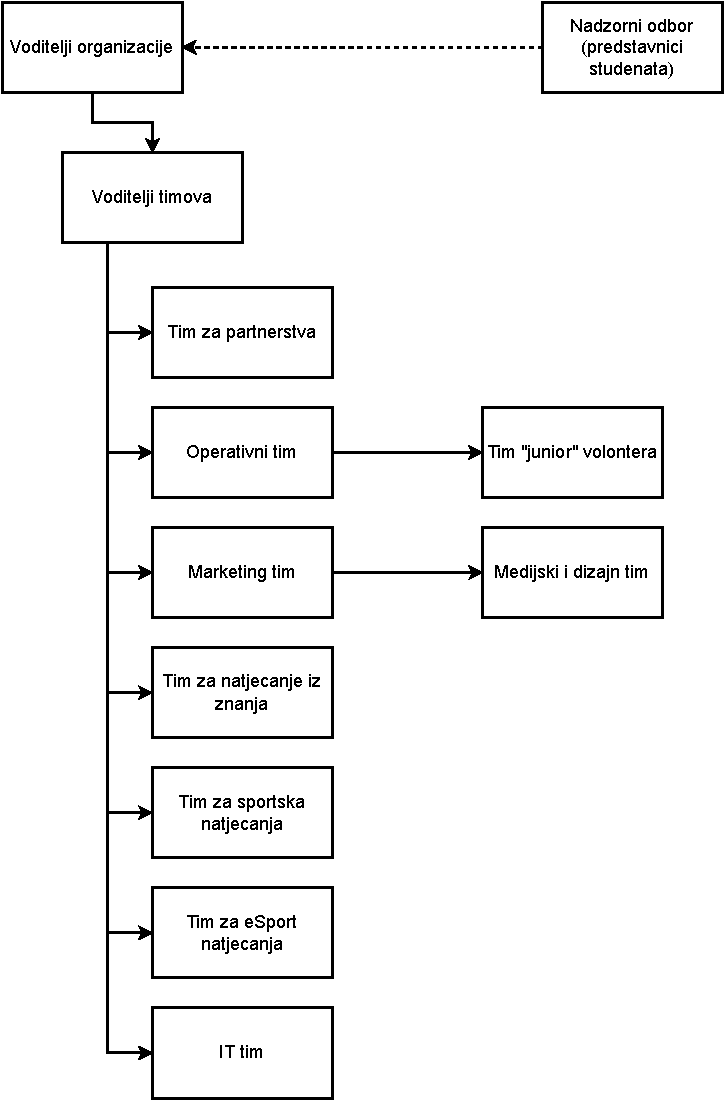
\includegraphics{slike/hijerarhija.pdf}
\caption{Prikaz organizacijskog ustroja}
\label{fig:hier}
\end{figure}

\section{Zadaci voditelja organizacije}
Voditelji organizacije, za koje su predviđene dvije pozicije u organizacijskoj
strukturi, započinju organizaciju projekta početkom akademske godine. Zaduženi
su, najprije, za okupljanje predstavnika studenata institucija koje će
sudjelovati.

Predstavnici onih institucija koje su dosad sudjelovale na natjecanju čine tzv.
\emph{nadzorni odbor} koji potvrđuje voditelje organizacije za tu godinu.
Voditelji organizacije potom digitalnim putem objavljuju natječaj za volontere u
organizaciji, od kojih se biraju drugi članovi organizacije uz potvrdu nadzornog
odbora.

Nakon ustroja organizacijskog tima, voditelji organizacije zaduženi su za
vremensko i resursno planiranje organizacije. Moraju voditi računa o
potencijalnim izvorima financiranja i rashodima potrebnima za organizaciju,
konzultirati nadzorni odbor o željama sudionika te ih uzeti u obzir prilikom
planiranja zadataka za organizacijske timove. Također, brinu se o suradnji s
kooperantom koji omogućuje prostor u kojem će se odvijati natjecanje te
posreduju u komunikaciji između ugostitelja i predstavnika institucija
sudionica.

Osim toga, voditelji organizacije brinu se o neprofitnoj organizaciji koja stoji
iza organizacijskog tima natjecanja. Brinu se o ispravnom bilježenju prihoda i
rashoda u suradnji s računovodstvenim servisom, ugovorima sa sponzorima i
kooperantima, održavanju skupština udruge i općenitim administrativnim poslovima
koji su za nju vezani.

\section{Zadaci studentskih predstavnika} \label{nadzorni}

Studentski predstavnici posreduju u komunikaciji između organizacijskog tima i
studenata visokoobrazovnih institucija koje sudjeluju na natjecanju. Prema
prethodnom sudjelovanju, neki od predstavnika studenata imaju pravo glasati o
pitanjima vezanim uz tijek organizacije. To čine digitalnim putem ili na
sastancima nadzornog odbora koje sazivaju voditelji organizacije.

Predstavnici također biraju studente koje će njihova institucija povesti na
natjecanje nakon što se studenti prijave preko jedinstvene stranice
organizacije. Zaduženi su i za organizaciju prijevoza sudionika na događaj te
eventualnog sufinanciranja njihovog sudjelovanja fakultetskim ili sponzorskim
subvencijama.

\section{Zadaci operativnog tima}

Operativni tim kao organizacijski tim u užem smislu ima veliki broj zadaća, te
je možda više od bilo kojeg drugog tima podložan informatizaciji. Glavne zadaće
operativnog tima su briga o nabavi, upravljanje inventarom, organizacija
lokalnog prijevoza, upravljanje timom "junior" volontera\footnote{volontera koji
    ne sudjeluju u organizaciji, ali pomažu fizički u provedbi samog događaja},
    organizacija dodatnog programa, akreditacija sudionika te briga o rasporedu
    događanja.

Detaljni zahtjevi na informacijski sustav od strane ovog tima, kao i drugih
timova, bit će opisani u nastavku, no ovdje vrijedi nešto detaljnije opisati
pojedinosti nabrojanih zadaća.

\subsection{Nabava i upravljanje inventarom}
Operativni tim vodi evidenciju o svim kooperantima s kojima je ostvarena
komunikacija tijekom tekućeg i prijašnjih projekata te prema tome ostvaruje
suradnje nužne za provedbu događaja. Ostali timovi iskazuju svoje potrebe za
nabavom materijala operativnom timu te članovi operativnog tima komuniciraju s
potencijalnim dobavljačima i dogovaraju nabavu. Nabavu u skladu s definiranim
budžetom odobravaju voditelji organizacije.

Veliki dio nabave potrebne za projekt odnosi se na tiskane materijale, koji se
tijekom događaja koriste za promociju sponzora i informiranje sudionika.
Prilikom nabave tiskanih materijala operativni tim mora, osim s dobavljačima,
komunicirati s \emph{timom za partnerstva} koji se brine o odobrenju materijala u
kojima se spominju sponzori događaja te \emph{medijskim i dizajn timom} koji
priprema grafičke pripreme.

Tijekom događaja, tim upravlja svim inventarom koji se koristi za provedbu
natjecanja. Brine o vlasništvu inventarskih stavki (one mogu biti posuđene, u
vlasništvu udruge, volontera ili ugostitelja), zaduženjima i ovlastima među
volonterima te lokacijama na kojima se pojedini predmeti u svakom trenutku
nalaze. Također brinu o prijevozu tih predmeta na lokaciju i njihovom povratku
vlasnicima.

\subsection{Lokalni prijevoz i prijevoz organizacije}

Jedan od zadataka operativnog tima također je osigurati prijevoz članova
organizacijskog tima na mjesto događaja. Pritom mora voditi računa o lokaciji
polaska različitih članova organizacije i rasporedu njihovog dolaska po danima.

Na lokaciji natjecanja mora brinuti o zaduženjima službenih vozila u najmu i
prioritetima za njihovo korištenje. Također, mora koordinirati autobusni
prijevoz sudionika u različitim komponentama natjecanja do sportskih dvorana ili
dvorana u kojima se odvija natjecanje u znanju.

\subsection{Upravljanje sudionicima}

Operativni tim zadužen je također za provedbu prijava sudionika preko web
sučelja na stranicama organizacije, komunicirajući pritom s predstavnicima
studenata o njihovim procedurama selekcije i kategorijama za koje žele otvoriti
prijave. Nakon selekcija provedenih od strane matičnih institucija sudionika,
operativni tim brine o njihovim osobnim podacima, izdaje ulaznice za događaj,
brine o njihovom dolasku i odlasku te posreduje u komunikaciji s ugostiteljskom
tvrtkom.

\subsection{Dodatni program, raspored i dodatni volonteri}

Uz glavni program natjecanja, na događanju STEM Games organizira se i dodatni
program u obliku neslužbenih natjecanja, predavanja i slično. Koordinacija tog
programa u smislu rasporeda, materijalnih i ljudskih resursa također je zadatak
operativnog tima.

Na samom događaju, osim članova organizacijskog tima, organizaciji pomažu i
volonteri u smislu fizičke i logističke potpore. Operativni tim zadužen je i za
vodstvo spomenutog tima volontera od kojih je svaki dužan utrošiti unaprijed
određeni broj sati dnevno na dodijeljena zaduženja. Jedna od zadaća volonterskog
tima je i prihvat sudionika na dolasku, pri čemu je brzina obrade pristiglog
sudionika vrlo važna i u čemu im informacijski sustav može pomoći.

\section{Zadaci tima za partnerstva}

Glavna zadaća partnerskog tima je omogućiti organizaciju događaja prikupljanjem
sredstava od sponzora u industriji. Zadaće ovog tima posebno su podložne
informatizaciji jer je za njihovo uspješno obavljanje potrebno pomno bilježiti
svu dosadašnju komunikaciju vezanu za ostvarene i potencijalne suradnje.

Organizacija sponzorima nudi uslugu promocije kroz izlaganje i distribuciju
promotivnih materijala te uključivanje u osmišljanje problemskog dijela
natjecanja. Te su usluge definirane kroz sponzorske pakete, koji ujedno
predstavljaju i moguće kategorije sponzora.

Rezultati rada partnerskog tima u obliku ugovora o suradnji sa sponzorima usko
su vezani uz financijske elemente organizacije te bi se stoga ta veza trebala
moći pratiti u potencijalnom dijelu informacijskog sustava vezanom uz
financijsko planiranje.

\section{Zadaci tima za marketing i komunikacije te podtimova}

Tim za marketing i komunikacije zadužen je za pružanje informacija o događaju
široj javnosti te njegovu promociju. Pritom se koristi web stranicom, profilima
na društvenim mrežama te medijskim partnerstvima. Svojim radom pruža vidljivost
kako samom događaju, tako i sponzorskim institucijama koje omogućuju financijska
sredstva za provedbu događaja. Pod taj tim također spadaju i timovi za grafički
dizajn i fotografiju koji se brinu za kreiranje materijala potrebnih za
promociju događaja.

S aspekta informatizacije, potrebe ovog tima svode se na praćenje ostvarenih i
potencijalnih kontakata s medijskim partnerima, katalogizaciju fotografskih i
video materijala te planiranje objava na kanalima digitalne komunikacije.

\section{Timovi za natjecanja u sportu, znanju i računalnim igrama}

Timovi za natjecanja bave se organizacijom sportskih i problemskih natjecanja te
natjecanja u računalnim igrama. Njihovi zadaci tiču se sastavljanja rasporeda,
zadataka za natjecatelje ili pripreme sportskih terena. Veći dio zadataka tih
timova nije relevantan za razvoj informacijskog sustava, pa time ne spada u
okvire ovog rada.

\section{Ostale potrebe}

Važan aspekt organizacijske strukture, a koji je zajednički svim timovima tiče
se upravljanja pravima pristupa. Iako se ne radi o konkretnom organizacijskom
zadatku, u svrhu potpunosti ovog opisa kao podloge za izolaciju zahtjeva, valja
navesti problematiku.

Navedeni se timovi u svom radu koriste raznim internetskim servisima. Neki od
tih servisa omogućuju individualnu registraciju korisnika, no kod nekih se
korisnički podaci za prijavu dijele među više osoba.

Posljedica te prakse je da se osjetljivi podaci dijele u kanalima koji za to
nisu predviđeni što uzrokuje sigurnosne rizike i poteškoće u praćenju korisnika
koji u nekom trenutku imaju pristup usluzi.

Informacijski bi sustav u ovom aspektu mogao omogućiti sigurno dijeljenje
pristupnih podataka prema potrebama i ovlastima članova organizacijskog tima. U
slučaju promjene osoba u ulogama ovlaštenim za pristup nekom servisu, zaporke bi
se mogle jednostavnije promijeniti jer bi sustav omogućio da se o toj promjeni
jednostavno obavijeste svi članovi tima koji koriste određeni servis.

Drugi aspekt kontrole pristupa je onaj fizički. Na samom događaju, uspostavljaju
se organizacijski ured i skladište kojemu mogu pristupiti samo određeni članovi
organizacije. Informatizacijom ovog aspekta pristup prostorima mogao bi se
kontrolirati digitalnim putem, korištenjem uređaja već ustaljenih za tu namjenu
poput RFID sustava, što bi otvorilo prostor za povećanu sigurnost u odnosu na
korištenje tradicionalnih metoda poput korištenja papirnatih akreditacija.

\chapter{Podaci organizacije za pohranu u IS} \label{reqs}

Nastavno na prethodni opis organizacije, a u svrhu ocjene prikladnosti ERP
sustava otvorenog koda i kasnijeg razvoja prilagođenog rješenja, valja
definirati potrebe organizacije koje bi informacijski sustav u primjeni trebao
zadovoljavati.

S obzirom na prirodu organizacijskih potreba, prioritetni zahtjevi na
informacijski sustav odnose se na pohranu podataka u sistematiziranom obliku te
se kroz rad organizacije potreba za njihovom obradom nije pokazala kao
prioritet. Slijedom toga, u aplikaciji se neće zahtijevati sloj poslovne
logike, te će se funkcionalni zahtjevi proučavati s aspekta podataka koje
aplikacija mora pohranjivati. Implicitno će se podrazumijevati da aplikacija
kroz svoje sučelje mora ponuditi operacije upisa, čitanja, modifikacije te
brisanja \engl{CRUD}, te da se prema pravilima organizacijske strukture za svaki
od definiranih podatkovnih entiteta može upravljati ovlastima kategorija
korisnika kojima je te operacije dopušteno izvoditi.

U ovom će poglavlju u svrhu analize zahtjeva opisno biti prikazane kategorije
podataka koje organizacija mora moći pohraniti u sustavu te njihovi međusobni
odnosi. Kako se od gotovih rješenja ne može očekivati podudarnost s potrebama
organizacije u idealnom slučaju, prije njihove ocjene njihove prikladnosti neće
se ulaziti u konkretne strukture podatkovnog modela, već će zahtjevi biti
razmotreni na višoj razini. Razrada i formalizacija konkretnog modela relacijske
baze podataka odgodit će se za poglavlje o rješenju korištenjem RAD programskog okvira.

\section{Podaci o osobama}

Organizacija natjecanja ovog tipa zahtjeva pohranu osobnih podataka velikog
broja različitih kategorija osoba povezanih s događajem. Imajući u vidu
osjetljivu prirodu osobnih podataka, vrlo je korisno omogućiti njihovu pohranu
na jednom mjestu, kako s aspekta informacijske sigurnosti tako i zbog
jednostavnosti upravljanja skupom podataka.

Osobni podaci koji se pohranjuju mogu pripadati članovima organizacijskog tima,
sudionicima natjecanja ili članovima drugih organizacija s kojima se surađuje
tijekom organizacije natjecanja. Ovisno o kategoriji pojedinca čiji se podaci
pohranjuju, tih podataka može biti više ili manje. Osnovni podaci uvijek su ime
i prezime osobe, kontakt podatak koji može biti adresa elektroničke pošte ili
broj telefona te pripadnost organizacijama i institucijama. Ovisno o potrebi,
tome se može nadodati datum rođenja, adresa stanovanja, neka vrsta jedinstvenog
identifikacijskog broja te u konkretnom slučaju opisane organizacije i veličina
majice, u svrhu izrade promotivnih materijala.

Uz osobne podatke, moraju se pratiti i podaci o sudjelovanju pojedinca na
konkretnom događaju. Ti će podaci biti opisani kasnije, ovisno o kategoriji
sudjelovanja osobe u pitanju.

\section{Korisnici sustava i uloge}

Neke od osoba čiji bi se podaci bilježili u sustavu istovremeno bi bili
korisnici tog sustava. U sustavu se moraju moći definirati korisnici uz svoje
pristupne podatke te se različite korisnike mora moći povezati sa zapisima o
njihovim osobnim podacima.

Svaki korisnik mora imati definirana prava pristupa različitim podacima
pohranjenim u sustavu te prava njihove izmjene u smislu operacija upisa,
modifikacije i brisanja. Kako se prava ne bi definirala pojedinačno za svakog
korisnika, u sustavu mora postojati koncept uloge kao skupa prava koji se može
unaprijed definirati i dodijeliti korisniku ovisno o njegovim organizacijskim
potrebama i ovlastima.

Svaki korisnik može imati više uloga te svaka uloga može biti pridružena većem
broju korisnika, a prava izmjene i dodjele uloga također su jedna od ovlasti
koja može biti omogućena jednoj od uloga. Ovakav pristup sigurnosti, poznat kao
RBAC \engl{role-based access control} vrlo je raširen (\cite{rbac}), te je stoga
izgledno da gotova rješenja nude takve mogućnosti.

\section{Podaci o organizacijama i institucijama}

Osim podataka o osobama uključenim u organizaciju događaja, važno je pohraniti
podatke o raznovrsnim organizacijama i institucijama koje su važne za njegovu
provedbu. To uključuje obrazovne institucije, sponzore, medijske partnere,
kooperante te partnerske organizacije.

Većina podataka o organizaciji ovisi o prirodi angažmana te organizacije unutar
projekta, te će stoga biti pobrojani u kasnijim potpoglavljima. Jedini obavezni
podatak u zapisu o pojedinoj organizaciji je njezino ime, a dodatni
(fakultativni) podaci uključuju adresu sjedišta organizacije, njezin matični
broj, relaciju prema kontakt osobama, generički kontakt organizacije te podatke
o njezinom angažmanu na pojedinim projektima, poželjno u obliku relacije prema
odvojenom zapisu o njezinom sudjelovanju.

\section{Podaci o projektima}

Svaki projekt, odnosno događanje koje se organizira, mora se moći zabilježiti u
informacijskom sustavu uz svoje predviđene datume početka i završetka. U zapisu
projekta nema potrebe za navođenjem ostalih podataka, ali se putem relacijskih
veza moraju moći dohvatiti različiti zapisi koji se odnose na pojedini projekt.

Ti će zapisi biti nabrojani u nastavku, a uključuju dokumente, budžet, ugovore i
račune, sponzorstva, sudjelovanja osoba, kooperante i vezane podatke.

\section{Podaci o sudjelovanju obrazovne institucije}

Osnovni podaci svake obrazovne institucije koja sudjeluje na natjecanju moraju
biti zapisani u dijelu informacijskog sustava koji pohranjuje podatke o
organizacijama i institucijama, no kao odvojenu kategoriju treba pohraniti i
podatke o njihovom sudjelovanju na konkretnom projektu. Ti podaci uključuju
relaciju prema projektu na kojem sudjeluju, relaciju prema osobama koje
ispunjavaju ulogu predstavnika studenata za tu godinu, procjenu broja sudionika,
broj glasova u nadzornom odboru na koji ta institucija eventualno ima pravo,
te kategorije natjecanja u kojima želi sudjelovati.

Poželjno je da zapis o sudjelovanju obrazovne institucije bude izravno povezan
sa zapisima o sudjelovanju njenih studenata na konkretnom natjecanju na koje se
zapis o sudjelovanju odnosi.

\section{Podaci o inventaru}

Informacijski sustav mora omogućiti pohranu podataka o inventaru dostupnom
organizaciji, koji može biti u vlasništvu organizacije, privatne osobe ili
pravne treće osobe. Zapis o inventarskoj stavci, dakle, mora sadržavati ime te
stavke po kojem ju se može identificirati, jedinstveni numerički identifikator,
oznaku lokacije relaciju prema zapisu o vlasniku (osobi ili organizaciji) te
relaciju prema osobi trenutno zaduženoj za brigu o stavci.

Dodatno, treba postojati mogućnost otpisa stavke, što može provesti brisanjem
stavke ili označavanjem polja koje ukazuje na status otpisa. Koristeći tu
mogućnost, zapisi o inventaru mogu se primijeniti i za praćenje potrošne robe.

\section{Podaci o dokumentu}

Uz fizički inventar organizacije, važno je pratiti i dokumente koji su od
organizacijskog značaja. To mogu biti financijski, pravni ili organizacijski
dokumenti, a glavni atributi zapisa o njima su naslov dokumenta, autor, vrijeme
nastanka te lokacija (fizička ili virtualna) na kojoj se dokument nalazi.

Uz to, u svrhu lakšeg pretraživanja dokumenata, bilo bi korisno omogućiti upis
kratkog opisa dokumenta.

\section{Podaci o sponzoru}

Prilikom komunikacije sa sponzorskim organizatorima, bilježenje povijesti
kontakata može biti od velike pomoći partnerskom timu koji osigurava sredstva za
održavanje događaja. Stoga je u informacijskom sustavu za potporu
organizacijskom timu, potrebno omogućiti pohranu podataka o suradnji s pojedinom
sponzorskom organizacijom.

Zapis o sponzorstvu poželjno bi relacijski bio vezan uz pojedini projekt i
organizaciju, a sadržavao bi razinu interesa koju je sponzor iskazao, kratki
opis sponzora, komentare o korespondenciji te relacijsku veze prema volonteru koji
je odgovoran za komunikaciju sa sponzorom i eventualnim sklopljenim ugovorima.

Takav zapis omogućio bi detaljni uvid u povijest suradnje s pojedinim sponzorom
u bilo kojem trenutku.

\section{Podaci o sudjelovanju natjecatelja}

Uz prijavu sudionika natjecatelja, za koju je važno imati zapis u informacijskom
sustavu, osim osobnih podataka vežu se i podaci vezani uz sudjelovanje te osobe
na pojedinom natjecanju. Ti podaci odnose se na kategorije u kojima se sudionik
natječe, identifikacijsku oznaku tima za one discipline u kojima se natječu
timovi te fakultativno smještajnu jedinicu u kojoj je sudionik smješten.

\section{Podaci o sudjelovanju volontera}

Važna organizacijska informacija jest i interni ustroj organizacije. S obzirom
na praksu da na različitim projektima ista osoba može obavljati različite uloge,
praktična funkcionalnost sustava bila bi da se za osobu koja radi na konkretnom
projektu može odrediti njezina funkcija kroz pripadnost timu.

Zbog različitih zadataka koje članovi istog tima mogu obavljati, ovaj je koncept
odvojen od uloge u smislu ovlasti korisnika sustava. Bilo bi, dakle, poželjno da
sustav omogućuje pohranu zapisa o pripadnosti pojedine osobe projektnim timovima
te povezivanje tog zapisa sa zapisom o izravno nadređenom volonteru ako takav
postoji.

\section{Podaci o računima}

Iako se o knjigovodstvu organizacije brinu za to stručni kooperanti, zbog
interne evidencije sustav treba omogućiti osnovno praćenje izlaznih i ulaznih
faktura. Izlazne fakture obično su vezane uz sponzore, a ulazne fakture uz
kooperante. Uz to, svaka je faktura dokument, te bi zapisi o fakturama morali
biti vezani uz pripadajuće zapise o dokumentima.

Svaki zapis o fakturi trebao bi sadržavati fakturirani iznos, datum izdavanja,
datum dospijeća i podatak o tome je li plaćanje izvršeno. Dodatno, zapisi o
izlaznim fakturama trebali bi sadržavati broj pod kojim je faktura izdana.

\section{Podaci o vozilima}

Tijekom provedbe samog natjecanja, organizacija mora voditi evidenciju o
korištenju vozila koje uzima u najam. Stoga bi bilo korisno omogućiti praćenje
planiranih i obavljenih vožnji vezanih uz pojedino vozilo.

Sustav bi u tu svrhu morao omogućiti upisivanje zapisa o vozilu te povezivanje
tog zapisa sa zapisima o rezervacijama vozila za planirane vožnje kao i zapisima
o obavljenim vožnjama. Svaki zapis o vožnji morao bi biti vezan uz osobu vozača,
polazište i odredište te vrijeme polaska i povratka.

Koristan dodatak zapisima o vožnjama bio bi podatak o stanju spremnika za gorivo
kako bi se za to zaduženim osobama omogućilo da na vrijeme opskrbe vozilo
gorivom.

\section{Podaci o budžetu}

Uz svaki projekt, veže se i plan raspodjele očekivanih sredstava. Sustav mora
omogućiti rudimentarno financijsko planiranje u obliku zapisa o kategoriji
troška te njegovom iznosu. Poželjna nadogradnja bila bi da se ulazne fakture
mogu povezati s nekim od zapisa u spomenutom planu, odnosno pojedinom budžetskom
stavkom.

\section{Podaci o kooperantima}

Na isti način kako partnerski tim bilježi podatke o sponzorima, operativni tim
trebao bi moći zabilježiti podatke o kooperantima. Zapis o kooperantu uključivao
bi komentare o prethodnoj suradnji, relacijsku vezu s relevantnim zapisom o
organizaciji te projektom na kojem se odvija suradnja te veze sa svim ulaznim
fakturama izdanim od strane spomenutog kooperanta.

\section{Pristupni podaci za mrežne usluge} \label{credential_problem}

Sustav bi također trebao omogućiti siguran prostor za pohranu pristupnih
podataka vezanih uz korisničke račune na internetskim servisima koje koristi
više osoba unutar organizacijskog tima. Svaki zapis o korisničkom računu mora
sadržavati ime servisa kojem se pristupa, korisničko ime i zaporku, a
relacijskom vezom mora biti ustanovljeno koje sve korisničke uloge imaju pravo
pročitati pojedini zapis.

Sustav mora ograničiti pristup ovim podacima samo na one uloge koje su za
korištenje tih podataka ovlaštene te lozinke mora pohranjivati u kriptografski
zaštićenom formatu.

\section{Podaci o medijskom partneru}

Naposljetku, sustav mora omogućiti praćenje kontakata i korespondencije s
medijskim partnerima događaja. Zahtjevi za ovu evidenciju identični su onima za
evidenciju sponzorstava, no s obzirom na to da se odnosima s medijima bavi drugi
tim, te dvije kategorije moraju biti razdvojene.

Dodatno, bilo bi poželjno omogućiti povezivanje medijskog partnera s medijskim
objavama koje su mu predložene. Zapis medijske objave tada bi trebao povezivati
zapis o dokumentu koji je izvorno izdao i poslao organizacijski tim, zapis o
medijskom partnerstvu te, ukoliko postoji, poveznicu na objavu od strane medija.

\chapter{Prikladnost \emph{ERP} sustava otvorenog koda}

Dio prethodno navedenih zadataka nije specifičan za organizaciju koja se bavi
studentskim natjecanjima te se sasvim sigurno može riješiti korištenjem gotovog
\emph{ERP} rješenja. S obzirom na velike troškove uvođenja komercijalnog
\emph{ERP} rješenja, studentske se organizacije mogu služiti jedino \emph{ERP}
rješenjima otvorenog koda.

\cite{erpstudy} u analizi devet takvih sustava zaključuje da, iako ih se
pojavljuje sve više, velikim dijelom nisu zadovoljavajuće kvalitete --- često su
loše dokumentirani, nestabilni ili neodržavani. Iskustvo autora pri proučavanju
\emph{ERP} sustava koji uključuju module namijenjene neprofitnim organizacijama
bilo je slično, te se kao jedina opcija vrijedna proučavanja nametnuo sustav
naziva \emph{ERPNext}

Sustav je dobro dokumentiran te za razliku od drugih rješenja otvorenog koda iza
njega stoji komercijalno poduzeće koje uz naplatu nudi i korisničku podršku.
Korisničko je sučelje intuitivno te se korištenjem \emph{Docker} sustava
\emph{ERP} paket može pustiti u rad na jednostavan način. Kontrola pristupa
pojedinim elementima sustava dobro je razrađena te omogućuje pripisivanje uloga
ili grupa uloga pojedinim korisnicima, od kojih svaka može sadržavati prava
pristupa pojedinom modulu. Sustav se također može integrirati s često korištenim
poslovnim aplikacijama, od kojih neke koristi i organizacija opisana u ovom
radu.

Očita prednost ovog sustava jest njegov modul za financije. Sustav
omogućuje planiranje, praćenje troškova i prihoda te automatsko izdavanje računa
koristeći obrasce zadane od strane korisnika. Mogućnosti ovoga sustava u
financijskom aspektu sasvim sigurno nadilaze mogućnosti koje se mogu ostvariti
koristeći \emph{RAD} programski okvir.

Sustav kroz svoje module za neprofitne organizacije omogućuje i praćenje članova
i volontera organizacije, no kako je namijenjen tradicionalnim neprofitnim
organizacijama ne nudi funkcionalnost bilježenja hijerarhijske strukture timova
prisutne u ovoj studentskoj organizaciji.

Kroz modul sustava namijenjen za upravljanjem klijentskim resursima, sustav
omogućuje i praćenje kontakata kooperanata i sponzora. Podatkovni model i
korisničko sučelje u ovom su modulu relativno složeni te bi njegova primjena
zahtijevala određenu edukaciju volontera korisnika, no to bi organizaciji moglo
biti od koristi. Kroz isti sustav mogla bi se pratiti komunikacija s medijskim
partnerima te bilježiti medijske objave.

Sustav također omogućuje praćenje inventara, no moduli za to daleko su
složeniji od potreba studentske organizacije. Namijenjeni su za praćenje
inventara velikih skladišta te uključuju pohranu brojnih nepotrebnih informacija
(poput informacija o transportu, vrijednosti i amortizaciji, rokovima trajanja i
slično). Primjena sustava u ovu svrhu uvela bi nepotrebne komplikacije te ne bi
donijela veliku dodatnu vrijednost za organizaciju.

U sustavu, očekivano, nedostaju mogućnosti za praćenje sudjelovanja studenata na
natjecanjima. Uz to, nedostaju mogućnosti praćenja vozila u posudbi te posuđenog
inventara, sudjelovanja obrazovnih institucija i pohrane pristupnih podataka za
internetske servise. Svaka od tih mogućnosti koje nedostaju mogla bi se
implementirati kao novi modul u sustavu koristeći programski okvir dokumentiran
u dokumentaciji sustava. Sustav se nadograđuje u programskom jeziku
\emph{Python} u kojem je i razvijen koristeći programski okvir \emph{Frappe}.

\chapter{Rješenje primjenom \emph{RAD} programskog okvira}
Kao drugi mogući pristup razmotrit će se informacijski sustav izrađen pomoću RAD
\engl{rapid application development} programskog okvira. Takav programski okvir
automatizira stvaranje obrazaca potrebnih za pohranu, pregled, uređivanje i
brisanje podataka \engl{CRUD} na temelju definiranog relacijskog podatkovnog
modela. Za razvoj informacijskog sustava koristeći takav programski okvir stoga
je dovoljno definirati podatkovni model, željene prikaze, odnose među njima te
eventualne nadogradnje u slučaju posebnih zahtjeva.

Pristup ovom problemu koristeći takav programski okvir prikladan je za
studentsku organizaciju u pitanju utoliko što korisnicima s malo tehničkih
znanja omogućuje jednostavan razvoj ili nadogradnju informacijskog sustava.
Pristup tog tipa posljednjih se godina sve više uspješno primjenjuje te je poznat pod
nazivom \engl{low-code} - s jedne strane pojednostavnjuje razvoj informacijskog
sustava, no istovremeno ograničava fleksibilnost krajnje funkcionalnosti
(\cite{low-code}).

Cilj ovog dijela rada je ispitati praktičnost primjene jednog takvog alata
razvijajući primjenjivu programsku podršku navedenim zahtjevima za slučaj
\emph{Udruge za studentska natjecanja STEM Games}. Razvijenom aplikacijom neće
biti pokriveni svi navedeni zahtjevi, već oni koji su za rad Udruge po osobnom
iskustvu autora važni te oni kroz koje se mogu ilustrirati primjene različitih
mogućnosti koje nudi korišteni programski okvir. Time će se također nastojati
dokumentirati proces oblikovanja informacijskog sustava kako bi se studentima
volonterima olakšala njegova nadogradnja ili izmjena.

S tim ciljem, u nastavku ovog poglavlja najprije će biti razrađen relacijski
podatkovni model koji će, uzevši u obzir broj entiteta i veza, iz praktičnih
razloga biti prikazan i obrazložen kratkim opisom za svaku pripadajuću tablicu.
Potom će na pojedinačnim primjerima biti opisan praktični aspekt implementacije
pomoću programskog okvira \emph{Flask-Appbuilder}, mogućnosti koje taj okvir
pruža te problemi i ograničenja s kojima se autor susreo. Naposljetku, na
nekoliko primjera bit će dokumentiran način puštanja u rad te korištenja
razvijene aplikacije.

\section{Entiteti podatkovnog modela} \label{model}

U ovom potpoglavlju bit će opisani entiteti podatkovnog modela aplikacije
razvijene korištenjem \emph{RAD} programskog okvira. Praktični aspekt definicije
podatkovnog modela korištenjem \emph{Flask-Appbuilder} knjižnica bit će
detaljnije razmotren u sljedećem poglavlju, no ovdje valja spomenuti da se
isti određuje u objektnom obliku kroz kod u programskom jeziku \emph{Python}.

Za svaki od entiteta definira se razred kojega knjižnica za objektno relacijsko
preslikavanje \engl{ORM} potom prevodi u relacijske tablice. Stoga će u nastavku
entiteti biti navedeni kao takvi, pod engleskim imenima razreda pod kojima su
definirani u kodu. Za svaki od entiteta bit će navedeno kratko obrazloženje za
njegovo uvođenje, opis njegovih atributa i veze prema drugim entitetima.

Veze između entiteta bit će navedene u opisu onog entiteta koji pohranjuje
strani ključ druge strane veze. U slučaju relacija \emph{više prema više}
\engl{many-to-many}, veza će biti navedena u opisu oba povezana entiteta.

\subsection{Entitet \emph{Project}} \label{project}

Ovaj se entitet odnosi na jedan projekt \emph{Udruge}. Konkretna udruga za koju
je razvijen model svake godine organizira jedno studentsko natjecanje koje je
zasebni projekt te se brojni podaci koje sustav mora moći pohraniti povezuju s
konkretnim projektom, što će biti navedeno u opisima odgovarajućih entiteta u
nastavku.

\medskip
Atributi ovog entiteta su:
\begin{itemize}
    \item \texttt{id} -- primarni ključ
    \item \texttt{name} -- ime projekta
\end{itemize}

\subsection{Entitet \emph{Organization}} \label{organization}

Ovaj entitet odnosi se na organizaciju bilo kojeg tipa s kojom je \emph{Udruga} u nekom
trenutku ostvarila suradnju ili planira ostvariti suradnju. Takva organizacija
među ostalim može biti sponzor, kooperant ili obrazovna institucija, a
eventualni detalji suradnje ili sudjelovanja pohranjeni su koristeći za to
predviđene entitete koji su povezani s ovim.

\medskip
Atributi ovog entiteta su:
\begin{itemize}
    \item \texttt{id} -- primarni ključ
    \item \texttt{name} -- ime organizacije
    \item \texttt{address} -- adresa organizacije (neobavezno)
    \item \texttt{generic\_email} -- kontakt elektroničke pošte organizacije
        (neobavezno)
    \item \texttt{oib} -- OIB organizacije (neobavezno)
\end{itemize}

\subsection{Entitet \emph{Person}} \label{person}

Ovaj entitet pohranjuje podatke o svim osobama povezanim s \emph{Udrugom}.
Slično kao i s entitetom vezanim uz organizacije, takva osoba može biti
sudionik, volonter, kontakt osoba druge organizacije ili bilo tko drugi povezan
s radom \emph{Udruge}, a za pohranu eventualnih detalja sudjelovanja koriste se
za to predviđeni entiteti koji će biti opisani u nastavku.

\medskip
Atributi ovog entiteta su:
\begin{itemize}
    \item \texttt{id} -- primarni ključ
    \item \texttt{full\_name} -- ime i prezime
    \item \texttt{email} -- adresa el. pošte (neobavezno)
    \item \texttt{phone} -- kontakt broj telefona (neobavezno)
    \item \texttt{sex} -- spol
    \item \texttt{oib\_or\_pin} -- identifikacijski broj osobe (neobavezno)
\end{itemize}

\subsection{Entitet \emph{EduInstitution}} \label{edu_institution}

Ovaj entitet predstavlja obrazovnu instituciju. Povezuje se na entitet koji
predstavlja organizaciju te je predviđen da sadrži dodatne detalje o obrazovnoj
instituciji. U ovom modelu jedini je takav detalj kratica pod kojom se obrazovna
institucija vodi u radu \emph{Udruge}, no lako je zamisliti buduće nadogradnje
po potrebi poput logotipa, područja studija i slično.


\medskip
Atributi ovog entiteta su:
\begin{itemize}
    \item \texttt{id} -- primarni ključ
    \item \texttt{abbreviation} -- kratica imena
    \item \texttt{organization\_id} -- strani ključ pripadajuće organizacije
\end{itemize}

Ovaj entitet povezan je s entitetom \emph{Organization} (potpoglavlje
\ref{organization}). Jedna obrazovna institucija obavezno je povezana s jednom
organizacijom.

\subsection{Entitet \emph{OrganizationTeam}} \label{organization_team}

Ovaj entitet predstavlja tim u organizacijskoj strukturi. S obzirom na to da je
organizacijska struktura hijerarhijske naravi (vidi poglavlje \ref{structure}),
svaki tim može ili ne mora pripadati većem timu. Takva je stablasta struktura
postignuta relacijom entiteta prema samome sebi.

Na ovaj entitet ne vežu se članovi timova, već se za svaki projekt definiraju
timovi koristeći entitet \emph{ProjectOrganizationTeam} (vidi
\ref{project_organization_team}). Ideja u pozadini ovog entiteta je da se pomoću
njega definira organizacijska struktura koja je većim dijelom jednaka na svakom
projektu te da služi kao predložak za definiranje timova na pojedinačnim
projektima.


\medskip
Atributi ovog entiteta su:
\begin{itemize}
    \item \texttt{id} -- primarni ključ
    \item \texttt{name} -- ime tima
    \item \texttt{part\_of\_team} -- ključ nadređenog, većeg tima (neobavezno)
\end{itemize}

Ovaj entitet ima povratnu vezu prema samome sebi.

\subsection{Entitet \emph{ProjectOrganizationTeam}}
\label{project_organization_team}

Ovaj entitet predstavlja organizacijski tim koji radi na jednom projektu. Praksa
je \emph{Udruge} da se za svaki projekt okuplja novi organizacijski tim pa se
stoga pojavljuje potreba za praćenjem sudjelovanja volontera u različitim
timovima za svaki projekt. Posljedično, koristeći ovaj entitet bilježi se
sudjelovanje pojedinog volontera na pojedinom projektu.

\medskip
Atributi ovog entiteta su:
\begin{itemize}
    \item \texttt{id} -- primarni ključ
    \item \texttt{project\_id} -- strani ključ projekta kojem tim pripada
    \item \texttt{organization\_team\_id} -- strani ključ tima u organizacijskoj
        strukturi
\end{itemize}

Ovaj tim povezan je s entitetom \emph{OrganizationVolunteer} (vidi
\ref{organization_volunteer}) koji predstavlja volontera u organizaciji u
relaciji \emph{više prema više} putem pomoćnih tablica
\emph{volunteer\_team\_membership} i \emph{volunteer\_team\_leadership}. Prva od
te dvije tablice povezuje tim s njegovim regularnim članovima, a druga s
njegovim voditeljima. Jedan volonter može biti član ili voditelj više različitih
timova te jedan tim može imati više od jednog voditelja i, naravno, člana.

\subsection{Entitet \emph{OrganizationVolunteer}} \label{organization_volunteer}

Ovaj entitet predstavlja volontera u organizaciji. Volonter može biti član ili
voditelj jednog ili više projektnih timova (vidi potpoglavlja
\ref{project_organization_team} i \ref{organization_team}), te može biti aktivan
ili neaktivan.

\medskip
Atributi ovog entiteta su:
\begin{itemize}
    \item \texttt{id} -- primarni ključ
    \item \texttt{person\_id} -- strani ključ zapisa o osobi
\end{itemize}

Entitet je povezan s entitetom \emph{ProjectOrganizationTeam} kroz dvije
relacije \emph{više prema više} pomoću tablica spomenutih u potpoglavlju
\ref{project_organization_team}.

\subsection{Entitet \emph{InstitutionParticipation}}
\label{institution_participation}

Ovaj entitet predstavlja sudjelovanje obrazovne institucije na pojedinom
projektu. Istovremeno, uvodi vezu \emph{više prema više} između obrazovnih
institucija (vidi potpoglavlje \ref{edu_institution}) i projekata (vidi potpoglavlje
\ref{project}), no smatrat će se entitetom zbog logike aplikacije te činjenice da
također sadržava broj glasova koje pojedina institucija ostvaruje na projektu
(vidi potpoglavlje \ref{nadzorni}). Ostaje također predviđena mogućnost da se
ovaj entitet proširi drugim podacima o sudjelovanju institucije u slučaju da se
za tim pokaže potreba.

\medskip
Atributi ovog entiteta su:
\begin{itemize}
    \item \texttt{id} -- primarni ključ
    \item \texttt{vote\_number} -- broj glasova institucije (0 ili više)
    \item \texttt{project\_id} -- strani ključ projekta
    \item \texttt{edu\_institution\_id} -- strani ključ obrazovne institucije
\end{itemize}

Ovaj je entitet povezan s entitetima \emph{Project} (potpoglavlje \ref{project})
i \emph{EduInstitution} (potpoglavlje \ref{edu_institution}).

\subsection{Entitet \emph{InstitutionRepresentation}}
\label{institution_representation}

Ovaj entitet predstavlja predstavnike studenata neke obrazovne
institucije.\footnote{Funkcija predstavnika objašnjena je u potpoglavlju
    \ref{nadzorni}.}. Svaka institucija može imati jednog ili više predstavnika,
    a predstavnik može biti glavni predstavnik ili zamjenik.


\medskip
Atributi ovog entiteta su:
\begin{itemize}
    \item \texttt{id} -- primarni ključ
    \item \texttt{edu\_institution\_id} -- strani ključ obrazovne institucije
    \item \texttt{person\_id} -- strani ključ zapisa o osobi
    \item \texttt{main\_representative} -- oznaka za predstavnike koji se
        smatraju "glavnima"
\end{itemize}

Ovaj je entitet povezan s entitetima \emph{EduInstitution} (potpoglavlje
\ref{edu_institution}) i \emph{Person} (potpoglavlje \ref{person}).

\subsection{Entitet \emph{Location}} \label{location}

Ovaj entitet predstavlja fizičku lokaciju relevantnu za rad \emph{Udruge}. U
trenutnom modelu, zapisi o lokaciji služe kako bi se uz nju vezale inventarske
stavke te fizički dokumenti, a predviđeno je da bi se na isti entitet mogli
nadovezati podaci o pravima pristupa fizičkim lokacijama ukoliko se u budućnosti
model proširi kako bi podržao i za to potrebne mehanizme.

\medskip
Atributi ovog entiteta su:
\begin{itemize}
    \item \texttt{id} -- primarni ključ
    \item \texttt{name} -- ime lokacije
    \item \texttt{address} -- adresa lokacije (neobavezno)
\end{itemize}

\subsection{Entitet \emph{InventoryItem}} \label{inventory_item}

Ovaj entitet predstavlja inventarsku stavku i služi za praćenje imovine
\emph{Udruge} ili imovine trećih osoba i organizacija koju \emph{Udruga} koristi
u svom radu. Za svaku stavku bilježi se vlasnik (osoba ili organizacija), osoba
koja je trenutno za nju odgovorna, te njezina lokacija. Također je predviđena
mogućnost otpisa stavke u slučaju njezinog gubitka ili oštećenja te kako bi se
isti entitet mogao koristiti za praćenje potrošnog materijala.

\medskip
Atributi ovog entiteta su:
\begin{itemize}
    \item \texttt{id} -- primarni ključ
    \item \texttt{name} -- ime stavke
    \item \texttt{owner\_organization\_id} -- strani ključ organizacije
        vlasnice (neobavezno)
    \item \texttt{owner\_person\_id} -- strani ključ osobe vlasnice (neobavezno)
    \item \texttt{responsible\_person\_id} -- strani ključ odgovorne osobe
    \item \texttt{location\_id} -- strani ključ lokacije na kojoj se stavka
        nalazi
    \item \texttt{discarded} -- oznaka otpisa
\end{itemize}

Ovaj entitet povezan je s entitetom \emph{Person} (potpoglavlje \ref{person})
dvama vezama, jednom koja predstavlja vlasnika i jednom koja predstavlja osobu u
čijem se zaduženju stavka trenutno nalazi. Također je povezan s entitetom
\emph{Organization} (potpoglavlje \ref{organization}) relacijom koja se koristi
u slučaju da je stavka u vlasništvu organizacije te s entitetom \emph{Location}
(potpoglavlje \ref{organization}) kako bi se omogućilo bilježenje fizičke
lokacije inventarske stavke.

\subsection{Entitet \emph{Sponsor}} \label{sponsor}

Ovaj entitet predstavlja sponzorstvo neke organizacije na nekom pojedinom
projektu, bilo ono ostvareno ili isključivo predloženo. Služi prvenstveno kako
bi se sačuvala sva povijest komunikacije sa sponzorima na projektima te se na
njega nadovezuju komentari vezani uz suradnju. Entitet također sadržava podatke
o otvorenosti sponzora za suradnju na konkretnom projektu te kategoriju
sponzorstva u slučaju da je suradnja ostvarena. Također sadrži podatak o osobi
unutar organizacije koja je zadužena za komunikaciju s konkretnim sponzorom te
se na njega vežu ugovori koji su s njime potpisani (vidi potpoglavlje
\ref{contract}).

\medskip
Atributi ovog entiteta su:
\begin{itemize}
    \item \texttt{id} -- primarni ključ
    \item \texttt{organization\_id} -- strani ključ organizacije sponzora
    \item \texttt{responsible\_person\_id} -- strani ključ osobe odgovorne za
        komunikaciju
    \item \texttt{project\_id} -- strani ključ projekta na koji se sponzorstvo
        odnosi
    \item \texttt{category\_id} -- strani ključ kategorije sponzorske suradnje
    \item \texttt{responsiveness\_id} -- strani ključ ocjene otvorenosti prema
        suradnji
\end{itemize}

Ovaj entitet povezan je s entitetima \emph{Organization} (potpoglavlje
\ref{organization}), \emph{Person} (potpoglavlje \ref{person}), \emph{Project}
(potpoglavlje \ref{project}), \emph{SponsorCategory} (potpoglavlje
\ref{sponsor_category}), te \emph{SponsorResponsivenessLevel} (potpoglavlje
\ref{sponsor_responsiveness_level}).

\subsection{Entitet \emph{SponsorComments}} \label{sponsor_comments}

Ovaj entitet predstavlja komentar bilo kakve vrste vezan uz suradnju s pojedinim
sponzorom na pojedinom projektu.

\medskip
Atributi ovog entiteta su:
\begin{itemize}
    \item \texttt{id} -- primarni ključ
    \item \texttt{comment} -- sadržaj komentara
    \item \texttt{sponsor\_id} -- strani ključ zapisa o sponzoru
\end{itemize}

Ovaj entitet povezan je s entitetom \emph{Sponsor} (potpoglavlje \ref{sponsor}).

\subsection{Entitet \emph{SponsorCategory}} \label{sponsor_category}

Ovaj entitet (šifrarnik) predstavlja moguće kategorije sponzorstva. Svaki
sponzor s kojim je ostvarena suradnja svrstava se u jednu od kategorija
sponzorstva.

\medskip
Atributi ovog entiteta su:
\begin{itemize}
    \item \texttt{id} -- primarni ključ
    \item \texttt{name} -- ime kategorije sponzorstva
    \item \texttt{description} -- opis kategorije sponzorstva
\end{itemize}

\subsection{Entitet \emph{SponsorResponsivenessLevel}}
\label{sponsor_responsiveness_level}

Ovaj entitet (šifrarnik) predstavlja otvorenost sponzora prema suradnji koju
sponzor može pokazati na određenom projektu. Ocjene se, koristeći ovaj entitet,
bilježe opisno te im se pridružuje brojčana vrijednost. U opis ocjene unose se
kriteriji koje sponzor ocijenjen tom ocjenom zadovoljava.

\medskip
Atributi ovog entiteta su:
\begin{itemize}
    \item \texttt{id} -- primarni ključ
    \item \texttt{name} -- ime ocjene
    \item \texttt{description} -- opis kriterija za ocjenu
    \item \texttt{score} -- proizvoljna brojčana vrijednost pridružena ocjeni
\end{itemize}

\subsection{Entitet \emph{Subcontractor}} \label{subcontractor}

Ovaj entitet predstavlja podugovorenu organizaciju, odnosno kooperanta.
Simetrično sa sponzorima (vidi potpoglavlje \ref{sponsor}), \emph{Udruga} prati
podatke o suradnji ostvarenoj s pojedinim kooperantom na pojedinom projektu.

\medskip
Atributi ovog entiteta su:
\begin{itemize}
    \item \texttt{id} -- primarni ključ
    \item \texttt{project\_id} -- strani ključ projekta
    \item \texttt{organization\_id} -- strani ključ organizacije kooperanta
\end{itemize}

Ovaj se entitet, dakle, veže na entitete \emph{Project} (potpoglavlje
\ref{project}) i \emph{Organization} (potpoglavlje \ref{organization}).

\subsection{Entitet \emph{SubcontractorComments}} \label{subcontractor_comments}

Ovaj entitet predstavlja komentar vezan uz suradnju s pojedinim kooperantom na
pojedinom projektu. To mogu biti iskustva s uslugom, pristupačnost, općeniti
zapisi o ostvarenim suradnjama i slično.

\medskip
Atributi ovog entiteta su:
\begin{itemize}
    \item \texttt{id} -- primarni ključ
    \item \texttt{comment} -- sadržaj komentara
    \item \texttt{subcontractor\_id} -- strani ključ zapisa o kooperantu
\end{itemize}

Ovaj entitet povezan je s entitetom \emph{Subcontractor} (potpoglavlje
\ref{subcontractor}).

\subsection{Entitet \emph{PhysicalDocument}} \label{physical_document}

Ovaj entitet predstavlja fizičku kopiju dokumenta od organizacijske važnosti.
Takav dokument može biti ugovor ili račun (detaljnije razrađeno u ovom
podatkovnom modelu, vidi potpoglavlja \ref{contract}, \ref{invoice_incoming} i
\ref{invoice_outgoing}) ili bilo kakav drugi dokument važan \emph{Udruzi}.
Entitet sadrži informacije o lokaciji kopije dokumenta, njegovom autoru, datumu
izrade te kratki opis sadržaja.

\medskip
Atributi ovog entiteta su:
\begin{itemize}
    \item \texttt{id} -- primarni ključ
    \item \texttt{name} -- ime ili naslov dokumenta
    \item \texttt{location\_id} -- strani ključ lokacije dokumenta
    \item \texttt{author\_id} -- strani ključ autora dokumenta (neobavezno)
    \item \texttt{date} -- datum izrade dokumenta
    \item \texttt{comment} -- kratki opis dokumenta (neobavezno)
\end{itemize}

Ovaj entitet povezan je s entitetom \emph{Person} (potpoglavlje \ref{person})
relacijom koja se odnosi na autorstvo te s entitetom \emph{Location}
(potpoglavlje \ref{location}).

Na ovaj entitet također se vežu prethodno spomenuti entiteti ugovora i
računa koristeći pomoćne tablice što je detaljnije opisano u navedenim
potpoglavljima vezanim uz te entitete.

\subsection{Entitet \emph{DigitalDocument}} \label{digital_document}

Ovaj entitet, kao i prethodni, predstavlja kopiju organizacijski značajnog
dokumenta, no u digitalnom obliku. Nalikuje entitetu \emph{PhysicalDocument}, no
umjesto navođenja fizičke lokacije kao referencu na dokument sadrži poveznicu na
njegovu virtualnu lokaciju.

\medskip
Atributi ovog entiteta su:
\begin{itemize}
    \item \texttt{id} -- primarni ključ
    \item \texttt{name} -- ime ili naslov dokumenta
    \item \texttt{link} -- poveznica na dokument
    \item \texttt{author\_id} -- strani ključ autora dokumenta (neobavezno)
    \item \texttt{date} -- datum izrade dokumenta
    \item \texttt{comment} -- kratki opis dokumenta (neobavezno)
\end{itemize}

Kao i prethodni, i ovaj entitet veže se na entitet \emph{Person} (potpoglavlje
\ref{person}) u svrhu zapisa autorstva dokumenta.

\subsection{Entitet \emph{InvoiceOutgoing}} \label{invoice_outgoing}

Ovaj entitet predstavlja izlazni račun, odnosno račun izdan od strane
\emph{Udruge} prema sponzoru. Svaki izlazni račun sastoji se od jedne ili više
stavki koje su predstavljene zasebnim entitetom (potpoglavlje
\ref{invoice_outgoing_item}), te se za njega bilježi tekstualna referenca,
datumi izdavanja i dospijeća, organizacija platitelj i podatak o tome je li
račun knjižen pri knjigovodstvenom servisu.

Iznos na koji se izdaje račun nije direktni atribut ovoga entiteta, već se on
računa kao zbroj iznosa svih stavki povezanih s računom. Takav pristup odabran
je kako bi se mogle bilježiti odvojene stavke te kako bi se ilustrirao mehanizam
izračunatih atributa kojega odabrani programski okvir nudi.

\medskip
Atributi ovog entiteta su:
\begin{itemize}
    \item \texttt{id} -- primarni ključ
    \item \texttt{name} -- ime računa (opisna referenca)
    \item \texttt{date\_issued} -- datum izdavanja računa
    \item \texttt{issue\_to\_id} -- strani ključ organizacije kojoj je račun
        izdan
    \item \texttt{date\_due} -- datum dospijeća računa (valuta plaćanja)
    \item \texttt{registered\_with\_accounting} -- oznaka da je račun knjižen
\end{itemize}

Ovaj je entitet, dakle, povezan s entitetom \emph{Organization} (potpoglavlje
\ref{organization}) kako bi se mogla zabilježiti organizacija kojoj je račun
izdan.

Dodatno, pomoćnim tablicama \emph{invoice\_outgoing\_digital\_copies}
i\linebreak \emph{invoice\_outgoing\_digital\_copies} ovaj je entitet povezan s
entitetima \emph{PhysicalDocument} (\ref{physical_document}) i
\emph{DigitalDocument} (\ref{digital_document}). Iako je veza u stvarnosti tipa
\emph{jedan prema više}, ostvarena je pomoćnim tablicama kako bi struktura
entiteta vezanih uz kopije dokumenata ostala nepromijenjena dodavanjem nove
vrste dokumenta.


\subsection{Entitet \emph{InvoiceOutgoingItem}} \label{invoice_outgoing_item}

Ovaj entitet predstavlja jednu stavku izlaznog računa. Stavka je jednostavni
podatak koji se sastoji od imena i vrijednosti, te je povezana s točno jednim
računom na kojem se nalazi.

\medskip
Atributi ovog entiteta su:
\begin{itemize}
    \item \texttt{id} -- primarni ključ
    \item \texttt{name} -- ime stavke
    \item \texttt{value} -- iznos (cijena) stavke
    \item \texttt{invoice\_outgoing\_id} -- strani ključ računa na kojemu se
        nalazi stavka
\end{itemize}

Ovaj entitet povezan je s entitetom \emph{InvoiceOutgoing} (potpoglavlje
\ref{invoice_outgoing}).

\subsection{Entitet \emph{InvoiceIncoming}} \label{invoice_incoming}

Ovaj entitet predstavlja ulazni račun, odnosno račun kojega je dužna podmiriti
\emph{Udruga}. Osmišljen je imajući na umu broj takvih računa o kojima treba
voditi evidenciju te je stoga pojednostavljen tako da ne sadržava informacije
koje za poslovanje \emph{Udruge} nisu relevantne.

Podaci o računu koji se bilježe kroz ovaj entitet su tekstualna referenca, datum
izdavanja, ime organizacije koja ga izdaje\footnote{Ovdje se iz praktičnih
    razloga račun ne povezuje s entitetom organizacije zbog velikog broja računa
    izdanih od strane organizacija za čijom evidencijom u sustavu nema potrebe.},
iznos za plaćanje, datum dospijeća i oznaka je li račun
knjižen pri knjigovodstvenom servisu. Ostavljen je također prostor za neobavezni
komentar te broj računa pod kojim se račun vodi kod isporučitelja.

\medskip
Atributi ovog entiteta su:
\begin{itemize}
    \item \texttt{id} -- primarni ključ
    \item \texttt{name} -- tekstualna referenca računa
    \item \texttt{date\_issued} -- datum izdavanja računa
    \item \texttt{vendor\_name} -- ime organizacije isporučitelja
    \item \texttt{vendor\_invoice\_number} -- broj računa (neobavezno)
    \item \texttt{value} -- ukupni iznos za plaćanje
    \item \texttt{date\_due} -- datum dospijeća
    \item \texttt{comment} -- tekstualni komentar (neobavezno)
    \item \texttt{registered\_with\_accounting} -- oznaka da je račun knjižen
\end{itemize}

Kao i u slučaju entiteta vezanog uz izlazne račune (vidi potpoglavlje
\ref{invoice_outgoing}) i ovaj entitet vezan je uz svoje fizičke i digitalne
kopije dvjema pomoćnim tablicama \emph{invoice\_outgoing\_physical\_copies} i
\emph{invoice\_outgoing\_digital\_copies}.

\subsection{Entitet \emph{Income}} \label{income}

Ovaj entitet predstavlja prihod koji je \emph{Udruga} ostvarila u nekom
trenutku. Prihod može ili ne mora biti vezan uz neki izlazni račun, te ima iznos
i datum ostvarivanja.

\medskip
Atributi ovog entiteta su:
\begin{itemize}
    \item \texttt{id} -- primarni ključ
    \item \texttt{name} -- tekstualni opis prihoda
    \item \texttt{value} -- iznos prihoda
    \item \texttt{date\_received} -- datum izvršenja transakcije
    \item \texttt{invoice\_incoming\_id} -- strani ključ ulaznog računa
        (neobavezno)
\end{itemize}

Ovaj je entitet, dakle, vezan za entitet \emph{InvoiceIncoming} (potpoglavlje
\ref{invoice_incoming}).

\subsection{Entitet \emph{Expense}} \label{expense}

Ovaj entitet predstavlja rashod (trošak) udruge. Slično kao prethodni entitet,
za svaki rashod bilježi se opis, ime i datum transakcije, te se rashod može
vezati uz ulazni račun. Dodatno, za rashod se bilježi i osoba koja ga je
odobrila.

\medskip
Atributi ovog entiteta su:
\begin{itemize}
    \item \texttt{id} -- primarni ključ
    \item \texttt{name} -- tekstualni opis prihoda
    \item \texttt{value} -- iznos prihoda
    \item \texttt{date\_paid} -- datum izvršenja transakcije
    \item \texttt{invoice\_outgoing\_id} -- strani ključ izlaznog računa
        (neobavezno)
    \item \texttt{approved\_by\_id} -- strani ključ osobe koja je odobrila
        rashod
\end{itemize}

Ovaj se entitet, dakle, veže uz entitete \emph{InvoiceOutgoing} (potpoglavlje
\ref{invoice_outgoing}) te \emph{Person} (potpoglavlje \ref{person}).

\subsection{Entitet \emph{PlannedIncome}} \label{planned_income}

Ovaj entitet odnosi se na prihod koji je planiran. Sadrži opis prihoda,
planirani iznos te planirani datum dospijeća prihoda. Ovaj entitet nije ni u
kakvom odnosu s drugim entitetima modela.

\medskip
Atributi ovog entiteta su:
\begin{itemize}
    \item \texttt{id} -- primarni ključ
    \item \texttt{name} -- tekstualni opis
    \item \texttt{value} -- novčani iznos
    \item \texttt{date\_planned} -- planirani datum transakcije
\end{itemize}

\subsection{Entitet \emph{PlannedExpense}} \label{planned_expense}

Ovaj se entitet odnosi na rashod koji je planiran. Njegova struktura identična
je onoj prethodnog entiteta te također nije ni u kakvoj vezi s ostalim
entitetima modela.

\medskip
Atributi ovog entiteta su:
\begin{itemize}
    \item \texttt{id} -- primarni ključ
    \item \texttt{name} -- tekstualni opis
    \item \texttt{value} -- novčani iznos
    \item \texttt{date\_planned} -- planirani datum transakcije
\end{itemize}

\subsection{Entitet \emph{Contract}} \label{contract}

Ovaj entitet odnosi se na ugovor koji je potpisan sa sponzorom na nekom
određenom projektu. S obzirom na to da entitet koji predstavlja sponzora
(potpoglavlje \ref{sponsor}) već sadrži podatak o projektu na kojeg se taj
sponzor odnosi, ovaj entitet ne bilježi direktno projekt na koji se odnosi.
Podaci koje sadrži ovaj entitet su ime ugovora, potpisnik, sponzor s kojim se
ugovor potpisuje, status (potpisan ili nepotpisan) te eventualna referenca na
račun izdan prema ugovoru.


\medskip
Atributi ovog entiteta su:
\begin{itemize}
    \item \texttt{id} -- primarni ključ
    \item \texttt{name} -- tekstualna referenca (ime) ugovora
    \item \texttt{sponsor\_id} -- strani ključ sponzora potpisnika ugovora
    \item \texttt{internal\_signee\_id} -- strani ključ osobe koja potpisuje
        ugovor unutar \emph{Udruge}
    \item \texttt{signed} -- status potpisa (potpisan ili nepotpisan)
    \item \texttt{invoice\_outgoing\_id} -- strani ključ računa izdanog prema
        ugovoru (neobavezno)
\end{itemize}

Ovaj je entitet povezan s entitetima \emph{Sponsor} (potpoglavlje
\ref{sponsor}), \emph{Person} (potpoglavlje \ref{person}) te
\emph{InvoiceOutgoing}. Veza prema entitetu \emph{Person} odnosi se na
internog potpisnika ugovora.

Dodatno, entitet je povezan s entitetima \emph{PhysicalDocument} (potpoglavlje
\ref{physical_document}) i \emph{DigitalDocument} (potpoglavlje
\ref{digital_document}) pomoćnim tablicama \emph{contract\_physical\_copies} i
\emph{contract\_digital\_copies} na isti način kako je to učinjeno za
račune.\footnote{Detalji ovakve veze objašnjeni su u potpoglavlju
    \ref{invoice_outgoing}.}

\subsection{Entitet \emph{OrganizationContact}} \label{organization_contact}

Ovaj entitet predstavlja kontakt osobu neke organizacije. Povezuje organizacije
i osobe, te sadrži podatak o ulozi osobe u organizaciji.

\medskip
Atributi ovog entiteta su:
\begin{itemize}
    \item \texttt{id} -- primarni ključ
    \item \texttt{organization\_id} -- strani ključ organizacije
    \item \texttt{contact\_person\_id} -- strani ključ osobe
    \item \texttt{role} -- tekstualni opis uloge osobe u organizaciji
\end{itemize}

Entitet se veže na entitete \emph{Organization} (potpoglavlje
\ref{organization}) i \emph{Person} (potpoglavlje \ref{person}).

\subsection{Entitet \emph{ParticipantInfo}} \label{participant_info}
Ovaj entitet predstavlja sudionika na jednom projektu. Povezuje se na entitet s
osobnim podacima sudionika te njima pridodaje podatke vezane za sudjelovanje
poput kategorije sudjelovanja, podatka o odobrenju sudjelovanja i veličine
majice\footnote{Veličina majice sudionika organizacijski je važan podatak zbog
    prakse tiska promotivnih majica.}. Zamišljeno je da se ovakav zapis vodi za
svaku osobu koja sudjeluje na nekom događaju u organizaciji \emph{Udruge}, a
zapis se može povezati s organizacijom u čijoj odgovornosti sudionik sudjeluje
ako takva postoji.

\medskip
Atributi ovog entiteta su:
\begin{itemize}
    \item \texttt{id} -- primarni ključ
    \item \texttt{person\_id} -- strani ključ osobe
    \item \texttt{project\_id} -- strani ključ projekta
    \item \texttt{responsible\_organization\_id} -- strani ključ organizacije
        odgovorne za sudionika (neobavezno)
    \item \texttt{participation\_approved} -- oznaka odobrenja sudjelovanja
    \item \texttt{participation\_approved\_by\_id} -- strani ključ osobe koja je
        odobrila (ili treba odobriti) sudjelovanje
    \item \texttt{participation\_approved} -- oznaka odobrenja sudjelovanja
    \item \texttt{participation\_category\_id} -- strani ključ kategorije
        sudjelovanja
    \item \texttt{t\_shirt\_size} -- veličina majice (tekst)
\end{itemize}

Entitet je dvostruko povezan s entitetom \emph{Person} (potpoglavlje
\ref{person}) --- jednom kako bi se zapis o sudioniku povezao s osobnim podacima
sudionika, a drugi put putem relacije koja označava osobu odgovornu za
odobrenje sudjelovanja konkretnog sudionika. Entitet je također vezan na entitete
\emph{Organization} (potpoglavlje \ref{organization}) te
\emph{ParticipationCategory} (potpoglavlje \ref{participation_category}).

\subsection{Entitet \emph{ParticipationCategory}} \label{participation_category}

Ovaj entitet (šifrarnik) definira moguće kategorije sudjelovanja sudionika.
Takva kategorija može biti natjecateljska ili nenatjecateljska.

\medskip
Atributi ovog entiteta su:
\begin{itemize}
    \item \texttt{id} -- primarni ključ
    \item \texttt{name} -- ime kategorije
\end{itemize}

\subsection{Entitet \emph{Vehicle}} \label{vehicle}

Ovaj entitet predstavlja vozilo kojim se koristi \emph{Udruga}. Vozilo može biti
u vlasništvu pojedinca ili organizacije (u slučaju najma ili posudbe). Entitet
sadrži ime vozila (kratki opis), njegovu registarsku oznaku te oznaku mogućnosti
rezervacije.

\medskip
Atributi ovog entiteta su:
\begin{itemize}
    \item \texttt{id} -- primarni ključ
    \item \texttt{name} -- ime vozila (kratki opis)
    \item \texttt{plate\_number} -- registarska oznaka vozila
    \item \texttt{available\_to\_reserve} -- označava je li moguća rezervacija
        vozila
    \item \texttt{owner\_person\_id} -- strani ključ fizičke osobe u čijem je
        vozilu vlasništvo (neobavezno)
    \item \texttt{owner\_organization\_id} -- strani ključ organizacije u čijem
        je vozilu vlasništvo (neobavezno)
\end{itemize}

\subsection{Entitet \emph{VehicleReservation}} \label{vehicle_reservation}

Ovaj entitet predstavlja rezervaciju vozila na događaju u organizaciji
\emph{Udruge}. Sadrži podatak o planiranom vremenu (početku i završetku
rezervacije) te neobavezno podatak o stvarnim vremenima preuzimanja i povrata
vozila.

\medskip
Atributi ovog entiteta su:
\begin{itemize}
    \item \texttt{id} -- primarni ključ
    \item \texttt{vehicle\_id} -- strani ključ vozila koje se rezervira
    \item \texttt{person\_id} -- strani ključ osobe koja rezervira
    \item \texttt{reservation\_start\_time} -- datum i vrijeme početka rezervacije
    \item \texttt{reservation\_end\_time} -- datum i vrijeme završetka
        rezervacije
    \item \texttt{vehicle\_taken\_time} -- datum i vrijeme preuzimanja vozila
        (neobavezno)
    \item \texttt{vehicle\_returned\_time} -- datum i vrijeme povrata vozila
        (neobavezno)
\end{itemize}

Entitet je povezan s entitetima \emph{Vehicle} (potpoglavlje \ref{vehicle}) i
\emph{Person} (potpoglavlje \ref{person}).

\subsection{Entitet \emph{ToolCredentials}} \label{tool_credentials}

Ovaj entitet predstavlja pristupne podatke za internetske servise te se njime
nastoji riješiti problem opisan u potpoglavlju \ref{credential_problem}. Entitet
sadrži ime servisa na koji se podaci odnose, korisničko ime (ukoliko ono
postoji) te zaporku koja se automatski pohranjuje u kriptiranom obliku.

\medskip
Atributi ovog entiteta su:
\begin{itemize}
    \item \texttt{id} -- primarni ključ
    \item \texttt{name} -- ime servisa na koji se odnose podaci
    \item \texttt{username} -- pristupno korisničko ime (neobavezno)
    \item \texttt{password} -- lozinka za pristup servisu (kriptirano)
\end{itemize}

Ovaj je entitet povezan s automatski generiranim entitetom \emph{Role} vezom
\emph{više prema više} o čemu će biti riječi u nastavku.

\subsection{Entiteti \emph{User}, \emph{Permission} i \emph{Role}} \label{user_and_role}

Programski okvir koji je korišten za izradu ove aplikacije nudi automatske
mehanizme za autorizaciju i kontrolu pristupa. Kao dio tih mehanizama, povrh
korisnički definiranog modela sam programski okvir uvodi entitete \emph{User},
\emph{Permission} i \emph{Role}.

Entitet \emph{User} odnosi se na jednog korisnika sustava i sadrži osnovne
podatke o korisniku te korisničko ime i
\emph{hash-vrijednost}\footnote{vrijednost koju poprima kriptografska
    jednosmjerna funkcija na argumentu jednakom lozinki} potrebnu za
autorizaciju korisnika.
Programski okvir pritom nudi mogućnost proširivanja entiteta \emph{User} što je u ovom
konkretnom modelu iskorišteno kako bi se zapis o korisniku povezao sa zapisom o
osobi u korisnički definiranom modelu.

Entitet \emph{Permission} predstavlja dozvolu korisniku da obavi određenu radnju
u sustavu. Programski okvir za svaki od definiranih entiteta automatski stvara
odvojene dozvole za svaku od \emph{CRUD} operacija kojima se potom može
upravljati iz korisničkog sučelja aplikacije. Automatski se stvaraju i dozvole
za prikaz pojedinih poveznica u izborniku korisničkog sučelja aplikacije te se
njihovim dodjeljivanjem korisnicima može upravljati izgledom korisničkog sučelja
koje će se pojedinom korisniku prikazati.

Entitet \emph{Role} predstavlja uloge koje korisnici mogu poprimati, odnosno
skupove dozvola definiranih kroz entitet \emph{Permission} koji se mogu
dodjeljivati korisnicima. Korisnik koji ima jednu ulogu poprima sve dozvole te
uloge, te je taj entitet vezan prema entitetu \emph{User} u odnosu \emph{više
prema više}.

Uz već spomenuto proširenje entiteta \emph{User} vezom prema entitetu
\emph{Person}, autorizacijski sustav programskog okvira \emph{Flask-Appbuilder}
u ovom je slučaju dodatno proširen vezom \emph{više prema više} prema entitetu
\emph{ToolCredentials}. Time se omogućava ograničavanje vidljivosti pojedinih
pristupnih podataka na samo neke uloge u sustavu.

\section{Implementacija pomoću \emph{Flask-Appbuilder} programskog okvira}

Prethodno opisani podatkovni model implementiran je u informacijskom sustavu
koristeći programski okvir \emph{Flask-Appbuilder}. Taj programski okvir
nadogradnja je na programski okvir \emph{Flask}, predviđen za razvoj web
aplikacija u programskom jeziku \emph{Python}. \emph{Flask-Appbuilder}, kako je
već spomenuto, automatizira veliki dio izrade aplikacije te je kompatibilan s
različitim sustavima relacijskih i \emph{NoSQL} baza podataka (\cite{fab}). Za
rad s relacijskim bazama podataka koristi se knjižnica za objektno relacijsko
preslikavanje \engl{ORM} \emph{SQLAlchemy} koja se može povezati s većinom često
korištenih relacijskih sustava baza podataka \engl{RDBMS} uključujući
\emph{SQLite}, \emph{Postgresql}, \emph{MySQL}, \emph{Oracle} i \emph{MS-SQL }
(\cite{sqlalchemy}). Upotreba takve knjižnice omogućuje definiciju podatkovnog
modela u \emph{Python} kodu te potpunu neovisnost o relacijskom sustavu baze
podataka u pozadini.

U nastavku će biti dokumentiran postupak implementacije informacijskog sustava
koristeći spomenuti programski okvir na pojedinačnim primjerima. Postupak se
sastoji od konfiguracije aplikacije, definicije podatkovnog modela te definicije
prikaza korisničkog sučelja \engl{ModelView}. Kroz pružene primjere nastojat će
se sažeto prikazati sve potrebne radnje za proširenje ili izmjenu razvijene
aplikacije prema budućim potrebama.

\subsection{Programska okolina} \label{environ}

Za razvoj aplikacije koristeći \emph{Flask-Appbuilder} ili njezino puštanje u
rad potrebno je osigurati odgovarajuću programsku okolinu. Preduvjet je, naravno
\emph{Python} prevoditelj \engl{interpreter} te programski paket
\emph{Flask-Appbuilder} sa svim paketima o kojima ovisi. Uz to, potrebna je neka
vrsta relacijskog sustava baza podataka \engl{RDBMS} koji će pohranjivati
podatke iz sustava te paket \emph{cryptography} potreban za pohranu kriptiranih
podataka (vidi potpoglavlje \ref{tool_credentials}).

Za potrebe ovog rada korišten je \emph{RDBMS SQLite} koji se isporučuje s
\emph{Python} prevoditeljem. U praktičnoj primjeni, bilo bi ga poželjno
zamijeniti robusnijim sustavom što se može postići izmjenom konfiguracijske
datoteke aplikacije spomenute u nastavku.

Programski paketi korišteni za razvoj aplikacije iz ovog rada mogu se
instalirati na sustav na kojemu je prisutan python prevoditelj pokretanjem
sljedeće naredbe:

\begin{lstlisting}[language=bash,basicstyle=\small\ttfamily,columns=flexible]
 > python -m pip install Flask-Appbuilder cryptography
\end{lstlisting}

\noindent koja će pokretanjem programa za upravljanje paketima instalirati dva
navedena paketa i sve pakete o kojima ovise.\footnote{Praksa je da se za
    instalaciju \emph{Python} okruženja aplikacija koriste tzv. virtualne
    okoline \engl{virtual environment}, no detalji tog pristupa izlaze iz opsega uputa
    u ovom radu.}

Paket Flask-Appbuilder \emph{Flask-Appbuilder} isporučuje se s pomoćnim alatom
\emph{fab} koji među ostalim omogućuje automatsko generiranje strukture datoteka
izvornog koda aplikacije, kreiranje relacijske baze podataka prema definiciji
modela te stvaranje početnog administratorskog korisnika (\cite{fab}). U slučaju
izrade nove aplikacije, kostur izvornog koda može se stvoriti pokretanjem
naredbe:

\begin{lstlisting}[language=bash,basicstyle=\small\ttfamily,columns=flexible]
 > flask fab create-app
\end{lstlisting}

\noindent čime će se pokrenuti interaktivni alat koji će stvoriti strukturu
direktorija i datoteka predviđenih za izvorni kod aplikacije (\cite{fab}).
Struktura paketa izvornog koda razvijenog tijekom izrade ovog rada prikazana je
u dodatku A ovom radu.

U slučaju pokretanja već razvijene aplikacije, nije potrebno izvršiti navedenu
naredbu. Kako bi se aplikacija pustila u rad, u konfiguracijskoj datoteci
\texttt{config.py} (vidi dodatak A) potrebno je postaviti putanju prema željenoj
bazi podataka:\footnote{Putanja mora biti u formatu kojega prihvaća
    \emph{SQLAlchemy ORM}. Format putanje opisan je u dokumentaciji programskog
    paketa te komentarima koje \emph{Flask-Appbuilder} automatski dodaje u
    konfiguracijsku datoteku.}
\begin{lstlisting}[language=python,basicstyle=\small\ttfamily,columns=flexible]
SQLALCHEMY_DATABASE_URI = <putanja prema bazi podataka>
\end{lstlisting}

Potom je potrebno izvršiti naredbu:
\begin{lstlisting}[language=bash,basicstyle=\small\ttfamily,columns=flexible]
 > flask fab create-db
\end{lstlisting}
\noindent koja će automatski generirati bazu podataka prema modelu definiranom u
datoteci izvornog koda \texttt{models.py} (vidi dodatak A) (\cite{fab}).

Naposljetku, valja dodati administratorskog korisnika korištenjem naredbe:
\begin{lstlisting}[language=bash,basicstyle=\small\ttfamily,columns=flexible]
 > flask fab create-admin
\end{lstlisting}
\noindent kojom se pokreće interaktivni alat kojim se može dodati novi
administrator (korisnik sustava kojemu su dodijeljene sve postojeće dozvole)
(\cite{fab}).

Nakon inicijalizacije, aplikacija je spremna za puštanje u rad. U razvojnoj
okolini, to se može postići naredbom:
\begin{lstlisting}[language=bash,basicstyle=\small\ttfamily,columns=flexible]
 > flask run
\end{lstlisting}
\noindent koja će pokrenuti ugrađeni \emph{HTTP} poslužitelj i početi
posluživati aplikaciju.

Prilikom puštanja aplikacije u rad u stvarnom okruženju, poželjno je ipak ne
koristiti poslužitelj ugrađen u \emph{Flask} programski paket već neki od
sigurnijih i robusnijih \emph{HTTP} poslužitelja (\cite{flask}). To je omogućeno
činjenicom da \emph{Flask} aplikacije odgovaraju specifikaciji \emph{WSGI}
\engl{Web Server Gateway Interface}. Ta specifikacija određuje sučelje za Web
aplikacije razvijene u \emph{Python} programskom jeziku koje im omogućuje
povezivanje s velikim brojem poslužiteljskih programa (\cite{pepwsgi}) poput
danas popularnih \emph{Apache} i \emph{Nginx}.

\subsection{Definicija modela}

U ovom potpoglavlju na nekoliko će primjera biti prikazan postupak definicije
entiteta u \emph{Python} kodu te će se kroz njih nastojati ilustrirati
funkcionalnosti \emph{SQLAlchemy} knjižnice korištene u razvoju aplikacije za
potrebe ovog rada.

Podatkovni model definiran je u datoteci \texttt{models.py} (vidi dodatak A).

\begin{lstlisting}[language=Python,basicstyle=\scriptsize,frame=single,caption={
kod entiteta \emph{Expense}},label={lst:expensemodel}]
class Expense(Model):
    id = Column(Integer, primary_key=True)
    name = Column(String(200), nullable=False)
    invoice_incoming_id = Column(Integer, ForeignKey('invoice_outgoing.id'))
    invoice_incoming = relationship('InvoiceIncoming', backref=backref('expense'))
    value = Column(Numeric, nullable=False)
    approved_by_id = Column(Integer, ForeignKey('person.id'), nullable=False)
    approved_by = relationship('Person')
    date_paid = Column(Date, nullable=False)

    def __repr__(self):
        return self.name
\end{lstlisting}

Iz isječka koda \ref{lst:expensemodel} vidljiv je osnovni princip definicije
entiteta.  Entitet se oblikuje kao \emph{Python} objekt izveden iz objekta
\emph{Model} kojega nudi paket \emph{SQLAlchemy}, a njegovi se atributi
definiraju kao atributi \emph{Python} razreda. Svakom atributu pridružuje se
objekt razreda \texttt{Column} koji definira pojedini atribut
(\cite{sqlalchemy}).

Rezultat ovakvog pristupa je razred čiji se objekti ponašaju kao obični
\emph{Python} objekti, a automatski su povezani s relacijskom bazom podataka u
pozadini. Ako nije izričito zadano drugačije, za svaki od takvih razreda u bazi
podataka stvorit će se odgovarajuća tablica čije ime odgovara imenu razreda uz
prilagodbu konvencije imenovanja (npr. \texttt{InvoiceIncoming} postat će
\texttt{invoice\_incoming}).

Na primjeru se može vidjeti i mehanizam ostvarivanja veza između entiteta.
Strani se ključevi definiraju kao i ostali atributi razreda, odnosno entiteta, a
potom se definiraju dodatni atributi razreda kojima se pridružuju veze
korištenjem funkcije \texttt{relationship}. Pristupanjem tim dodatnim atributima
unutar \emph{Python} koda pristupa se direktno objektu koji je povezan stranim
ključem.

Pri ostvarivanju takve veze, korištenjem funkcije \texttt{backref} može se
ostvariti i povratna veza. U konkretnom primjeru, korištenjem te funkcije
automatski se definira atribut \texttt{expense} na objektima razreda
\texttt{InvoiceIncoming}. Pristupanjem tom atributu iz \emph{Python} koda može
se dohvatiti povezani objekt razreda \texttt{Expense}, a u slučaju veza tipa
\emph{više prema jedan} ili \emph{više prema više} takvim postupkom dohvaća se
lista svih povezanih objekata. Definicija ovakvih povratnih veza u ovom se
slučaju direktno reflektira i na korisničko sučelje aplikacije gdje će se one
automatski prikazati.

\begin{lstlisting}[language=Python,basicstyle=\scriptsize,frame=single,caption={
kod entiteta \emph{InvoiceOutgoing}},label={lst:invoiceoutgoingmodel}]
class InvoiceOutgoing(Model):
    id = Column(Integer, primary_key=True)
    name = Column(String(200), nullable=False)
    date_issued = Column(Date, nullable=False)
    issued_to_id = Column(Integer, ForeignKey('organization.id'))
    issued_to = relationship('Organization')
    date_due = Column(Date, nullable=False)
    digital_copies = relationship('DigitalDocument',
        secondary=invoice_outgoing_digital_copies)
    physical_copies = relationship('PhysicalDocument',
        secondary=invoice_outgoing_physical_copies)
    registered_with_accounting = Column(Boolean)

    @hybrid_property
    def value(self):
        return sum(i.value for i in self.items)

    @value.expression
    def value(cls):
        return (
                select([func.sum(InvoiceOutgoingItem.value)]).
                where(InvoiceIncomingItem.invoice_incoming_id == cls.id).
                label('value')
                )
\end{lstlisting}

Isječak koda \ref{lst:invoiceoutgoingmodel} dodatno ilustrira dvije korištene
funkcionalnosti \emph{SQLAlchemy} paketa.

Prva je ostvarivanje veza korištenjem sekundarnih tablica (primjer definicije
takve tablice dan je u isječku koda \ref{lst:assoctable}), koje se navode kao
argument prethodno spomenute funkcije \texttt{relationship}.

Druga je korištenje tzv. \emph{hibridnih atributa} kojima se entitetu daje
virtualni atribut izračunat iz podataka prisutnih u bazi. Takav se atribut
ostvaruje dvjema definicijama metoda - u prvoj definiciji (označenoj dekoratorom
\texttt{hybrid\_property} definira se izraz
prema kojemu se virtualni atribut računa kad mu se pristupa iz \emph{Python}
koda, a u drugoj se isti izraz definira kao \emph{SQL} upit kako bi se njegov
rezultat mogao koristiti u složenijim upitima na bazu. \emph{ORM} paket na
takvom entitetu omogućava slaganje upita na transparentan način, odnosno
virtualni se atribut ponaša na potpuno isti način kao što bi se ponašao da se
radi o stvarnom atributu entiteta.

\begin{lstlisting}[language=Python,basicstyle=\scriptsize,frame=single,caption={
kod pomoćne tablice \emph{invoice\_outgoing\_digital\_copies}},label={lst:assoctable}]
invoice_outgoing_digital_copies = Table('invoice_outgoing_digital_copies',
        Model.metadata,
        Column('id', Integer, primary_key=True),
        Column('invoice_outgoing_id', Integer, ForeignKey('invoice_outgoing.id')),
        Column('digital_document_id', Integer, ForeignKey('digital_document.id'),
            unique=True))
\end{lstlisting}

\subsection{Definicija korisničkog sučelja}

Nakon definicije modela, potrebno je definirati prikaze korisničkog sučelja koji
će se prikazati korisnicima. Programski paket \emph{Flask-Appbuilder} taj
postupak krajnje pojednostavljuje.

Definicije prikaza korisničkog sučelja nalaze se u datoteci \texttt{views.py}
(vidi dodatak A).

\begin{lstlisting}[language=Python,basicstyle=\scriptsize,frame=single,caption={
kod prikaza \emph{SponsorModelView}},label={lst:modelview}]
class SponsorModelView(ModelView):
    datamodel = SQLAInterface(Sponsor)
    related_views = [SponsorCommentsModelView]
    show_template = 'appbuilder/general/model/show_cascade.html'

    list_columns = ['name']
\end{lstlisting}

Na primjeru u isječku koda \ref{lst:modelview} može se vidjeti oblik jedne takve
definicije. Za svaki prikaz definira se razred izveden iz razreda
\texttt{ModelView}. Taj se razred s podatkovnim entitetom povezuje putem atributa
\texttt{datamodel} što rezultira automatskim stvaranjem \emph{master-detail}
prikaza vezanog uz taj entitet u korisničkom sučelju koji nad njim omogućava
\emph{CRUD} operacije.

Prikazi se mogu međusobno povezivati koristeći atribut razreda
\texttt{related\_views}. Tom se atributu pridružuje lista drugih prikaza koji su
u nekom odnosu s entitetom na koji se prikaz odnosi, nakon čega će sustav
u \emph{detail} prikazu automatski omogućiti baratanje povezanim zapisima. Ovdje
valja napomenuti da povezani prikazi moraju biti definirani prije njihovog
navođenja u spomenutom atributu.

Dodatno, unutar atributa \texttt{list\_columns} potrebno je navesti sva
podatkovna polja koja će se pojaviti u tabličnom \emph{master} prikazu. Imena
polja ovdje se odnose na atribute entiteta. Također je moguće odabrati način
prikazivanja povezanih prikaza postavljanjem atributa \texttt{show\_template}, pri
čemu sustav nudi prikaz u karticama ili na istoj stranici.

\begin{figure}[H]
    \centering
    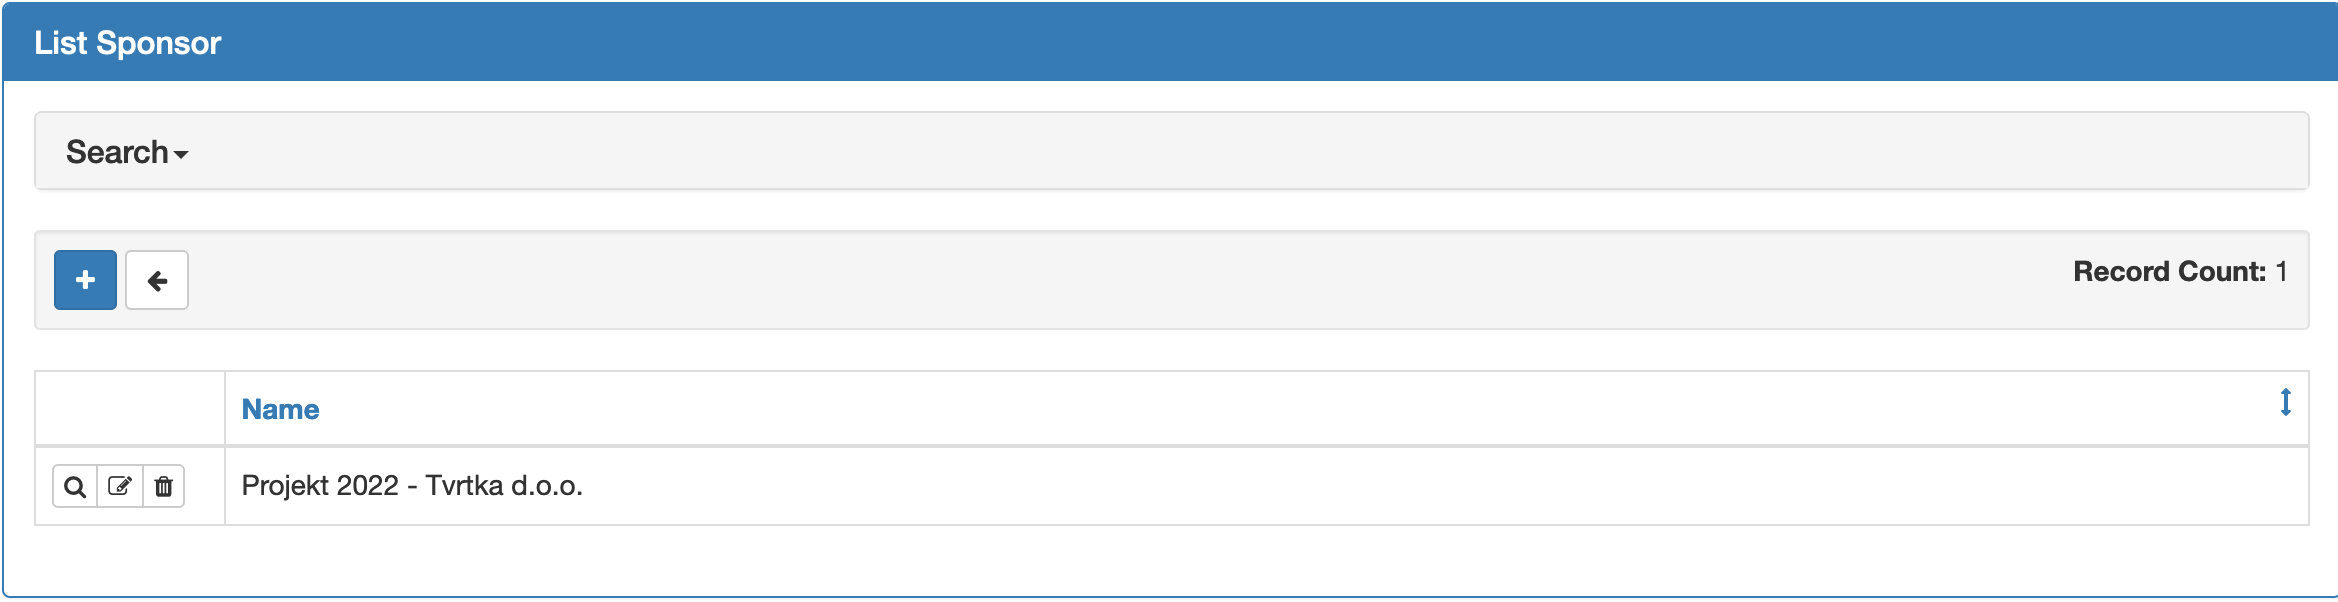
\includegraphics[width=1\textwidth]{slike/sponsormaster.png}
    \caption{\emph{Master} prikaz vezan uz entitet \texttt{Sponsor}}
    \label{fig:sponsormaster}
\end{figure}

\begin{figure}[H]
    \centering
    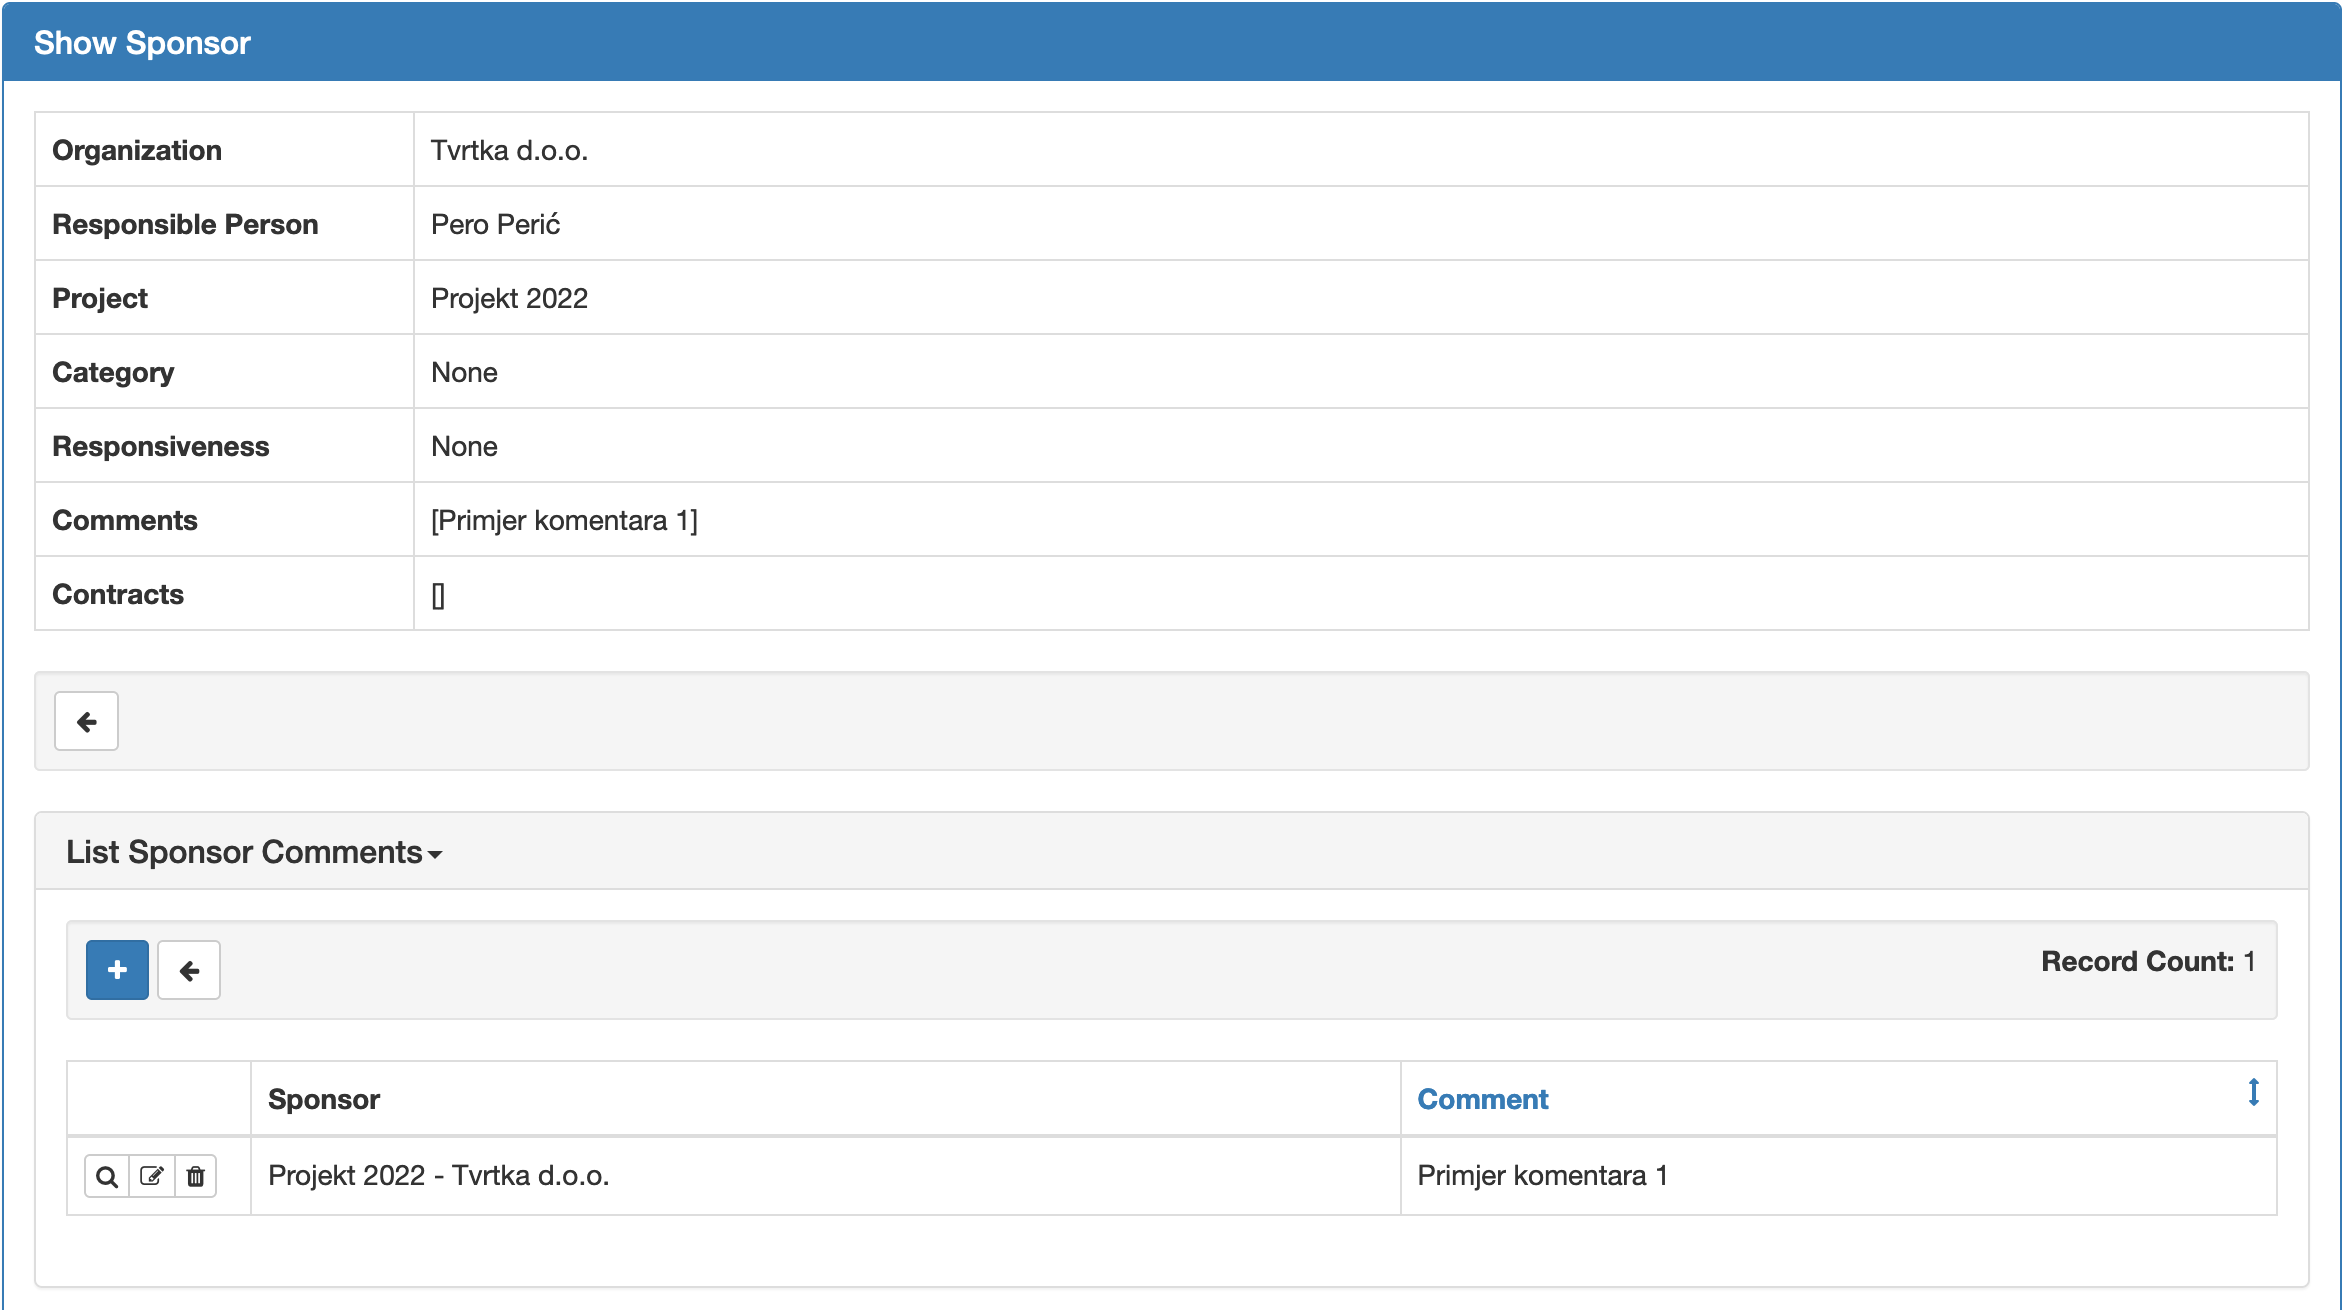
\includegraphics[width=1\textwidth]{slike/sponsordetail.png}
    \caption{\emph{Detail} prikaz vezan uz entitet \texttt{Sponsor}}
    \label{fig:sponsormaster}
\end{figure}

Na kraju je potrebno registrirati definirani prikaz te odrediti njegov položaj u
strukturi izbornika. To se postiže na način vidljiv u isječku koda
\ref{lst:mvreg}.

\begin{lstlisting}[language=Python,basicstyle=\scriptsize,frame=single,caption={
registracija prikaza},label={lst:mvreg}]
appbuilder.add_view(
        SponsorModelView,
        "Sponsors",
        icon = "fa-folder-open-o",
        category = "Partnerships",
        category_icon = "fa-handshake-o"
    )
\end{lstlisting}

\subsection{Filtriranje i kontrola pristupa} \label{acc_ctr}

Kao što je već spomenuto u potpoglavlju \ref{user_and_role}, na primjeru
entiteta \emph{ToolCredentials} proširen je sigurnosni sustav ugrađen u
\emph{Flask-Appbuilder}. Ugrađeni sigurnosni sustav omogućuje upravljanje
pravima pristupa registriranim prikazima (vidi prethodno potpoglavlje) te
pojedinačnim \emph{CRUD} operacijama, no ne omogućuje kontrolu pristupa
pojedinačnim zapisima u bazi podataka.

Stoga je u svrhu ograničavanja vidljivosti zapisa entiteta
\emph{ToolCredentials} potrebno uvesti dodatni mehanizam. U aplikaciji
razvijenoj za potrebe ovog rada, to je ostvareno uvođenjem relacije \emph{više
prema više} između entiteta \emph{ToolCredentials} i \emph{Role} koristeći
pomoćnu tablicu definiranu kao razred \emph{ToolCredentialPermission}.

Za tu tablicu definiran je posebni prikaz na način opisan u prethodnom poglavlju
koji omogućuje korisnicima koji za to imaju ovlasti da povezuju uloge u sustavu
s podacima za pristup pojedinom servisu. Prikaz entiteta \emph{ToolCredentials}
potom je definiran tako da podatke prije prikaza filtrira prema dozvolama uloga
koje su pripisane trenutnom korisniku.

To se može postići korištenjem atributa \texttt{base\_filter} prilikom
definiranja prikaza za taj entitet. Ova je mogućnost izrazito slabo
dokumentirana u dokumentaciji \emph{Flask-Appbuilder} paketa, no njezino je
korištenje ilustrirano u programskim primjerima dostavljenim s tim paketom. Iz
tog razloga, vrijedi izdvojiti i ukratko komentirati taj dio koda.


\begin{lstlisting}[language=Python,basicstyle=\scriptsize,frame=single,caption={
filtriranje pristupnih podataka},label={lst:filter}]
class CredentialsFilterFunction(BaseFilter):
    def apply(self, query, func):
        query, field = get_field_setup_query(query, self.model, self.column_name)
        return query.filter(field.any(ToolCredentials.id.in_(func())))

def get_user_allowed_credentials():
    return set(c.id for role in g.user.roles \
            for c in role.accessible_credentials)
...

class ToolCredentialsModelView(ModelView):
    datamodel = SQLAInterface(ToolCredentials)
    related_views = [ToolCredentialPermissionModelView]
    list_columns = ['tool_name', 'username', 'password']
    base_filters = [('have_access',
        CredentialsFilterFunction, get_user_allowed_credentials)]
\end{lstlisting}

Najprije treba definirati razred izveden iz razreda \texttt{BaseFilter}
definiranog u \emph{Flask-Appbuilder} programskom paketu. U tom razredu treba
definirati metodu \texttt{apply} koja prima \emph{SQLAlchemy} upit kao prvi
parametar i funkciju koja pri svojem pozivu vraća sve ključeve zapisa dostupnih
korisniku. Ta metoda mora vratiti upit nadopunjen željenim filterom.

Potom treba definirati funkciju koja će vratiti ključeve zapisa za pristup
trenutno prijavljenom korisniku, kojem se može pristupiti koristeći objekt
\texttt{g} dostupan u knjižnici \emph{Flask}. U ovom je to slučaju funkcija
\texttt{get\_user\_allowed\_credentials}.

Na kraju, u prikazu koji se filtrira treba definirati atribut razreda
\texttt{base\_filters} te u njemu navesti vezu po kojoj se filtrira, te
definirani razred i funkciju. Konkretna definicija može se vidjeti u isječku
koda \ref{lst:filter}.

Dodatno, sigurnosni mehanizam u ovoj je aplikaciji proširen i dodavanjem veze
između entiteta \emph{User} i \emph{Person} (vidi potpoglavlje
\ref{user_and_role}). Takvo proširenje postiže se definiranjem novih razreda
izvedenih iz razreda \emph{User} i \emph{UserModelView}, no taj postupak dobro
je dokumentiran u dokumentaciji programskog paketa \emph{Flask-Appbuilder} te
stoga njegov opis izlazi iz opsega ovog rada.

\section{Korištenje aplikacije}

U ovom potpoglavlju ukratko će biti opisan način korištenja razvijene
aplikacije. S obzirom na veliki broj već opisanih entiteta te kako bi se
izbjeglo ponavljanje, mogućnosti aplikacije bit će predstavljene na nekoliko
primjera podatkovnih entiteta pri čemu će se podrazumijevati da se s ostalim
entitetima postupa na jednak način.

\subsection{Glavno sučelje}

Otvaranjem početne stranice, neprijavljenom korisniku nudi se opcija za prijavu.
Sučelje za prijavu korisnika \emph{Flask-Appbuilder} generira automatski, a
početni administratorski korisnik može se registrirati koristeći naredbe iz
potpoglavlja \ref{environ}.

\emph{Flask-Appbuilder} nudi i automatsko sučelje za samostalnu registraciju
korisnika, no u ovoj primjeni ta mogućnost nije korištena jer nije poželjno
omogućiti registraciju neovlaštenih korisnika.

\begin{figure}[H]
    \centering
    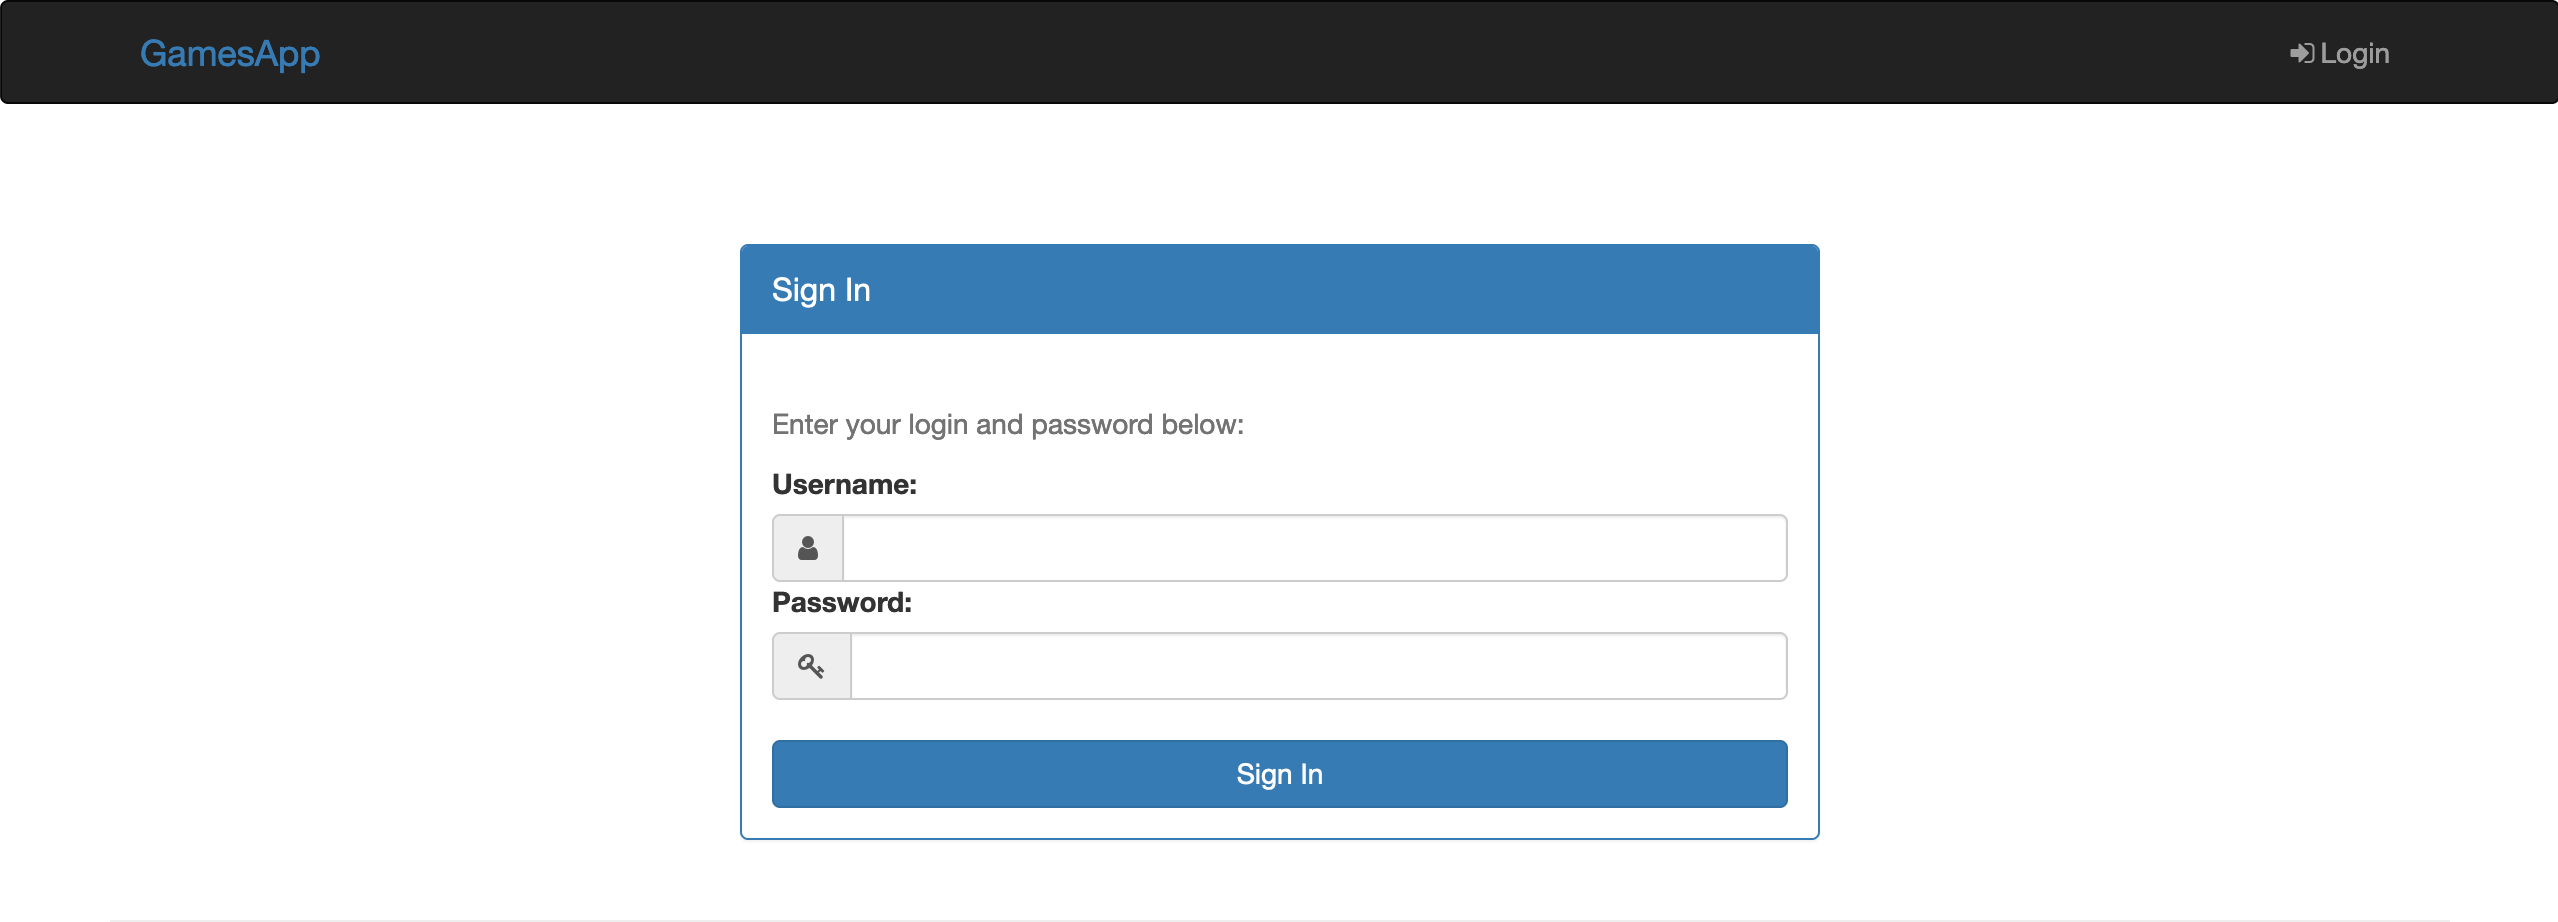
\includegraphics[width=1\textwidth]{slike/loginscreen.png}
    \caption{Sučelje za prijavu korisnika}
    \label{fig:loginscreen}
\end{figure}

Nakon prijave, korisniku se prikazuje početna stranica s alatnim izbornikom.
Opcije dostupne u izborniku za pojedinog korisnika mogu se ograničiti izborom
odgovarajuće uloge ili dozvola unutar uloge, a administratorskom korisniku
prikazat će se sve dostupne opcije.

\begin{figure}[H]
    \centering
    
\includegraphics[width=1\textwidth]{slike/adminmain.png}
    \caption{Početna stranica administratora}
    \label{fig:adminmain}
\end{figure}

U alatnom izborniku dostupni su svi prikazi registrirani u datoteci
\texttt{views.py} kojima je trenutnom korisniku dozvoljeno pristupiti. U ovoj
aplikaciji, takav je prikaz definiran za svaki od entiteta opisanih u
potpoglavlju \ref{model}.

Prikazi su podijeljeni u nekoliko kategorija, odnosno izbornika. U dodatku B
rada mogu se vidjeti svi dostupni izbornici.

Dodatno, u alatnoj se traci pojavljuje i izbornik \emph{Security} koji omogućuje
upravljanje ugrađenim mehanizmima kontrole pristupa. U taj izbornik u razvijenoj
aplikaciji dodan je i prikaz \emph{Tool Credential Permissions} kojim se
upravlja pravima pristupa zapisima u prikazu \emph{Tool Credentials}.

\subsection{Upravljanje korisnicima, dozvolama i ulogama}

Administrator nakon početka korištenja aplikacije mora definirati uloge
korisnika u sustavu te dodati korisnike. Ovlasti koje se mogu pripisati
određenoj ulozi unaprijed su prisutne u sustavu, a ulogama se može upravljati
odabirom opcije \emph{List Roles} iz izbornika \emph{Security}.

\begin{figure}[H]
    \centering
    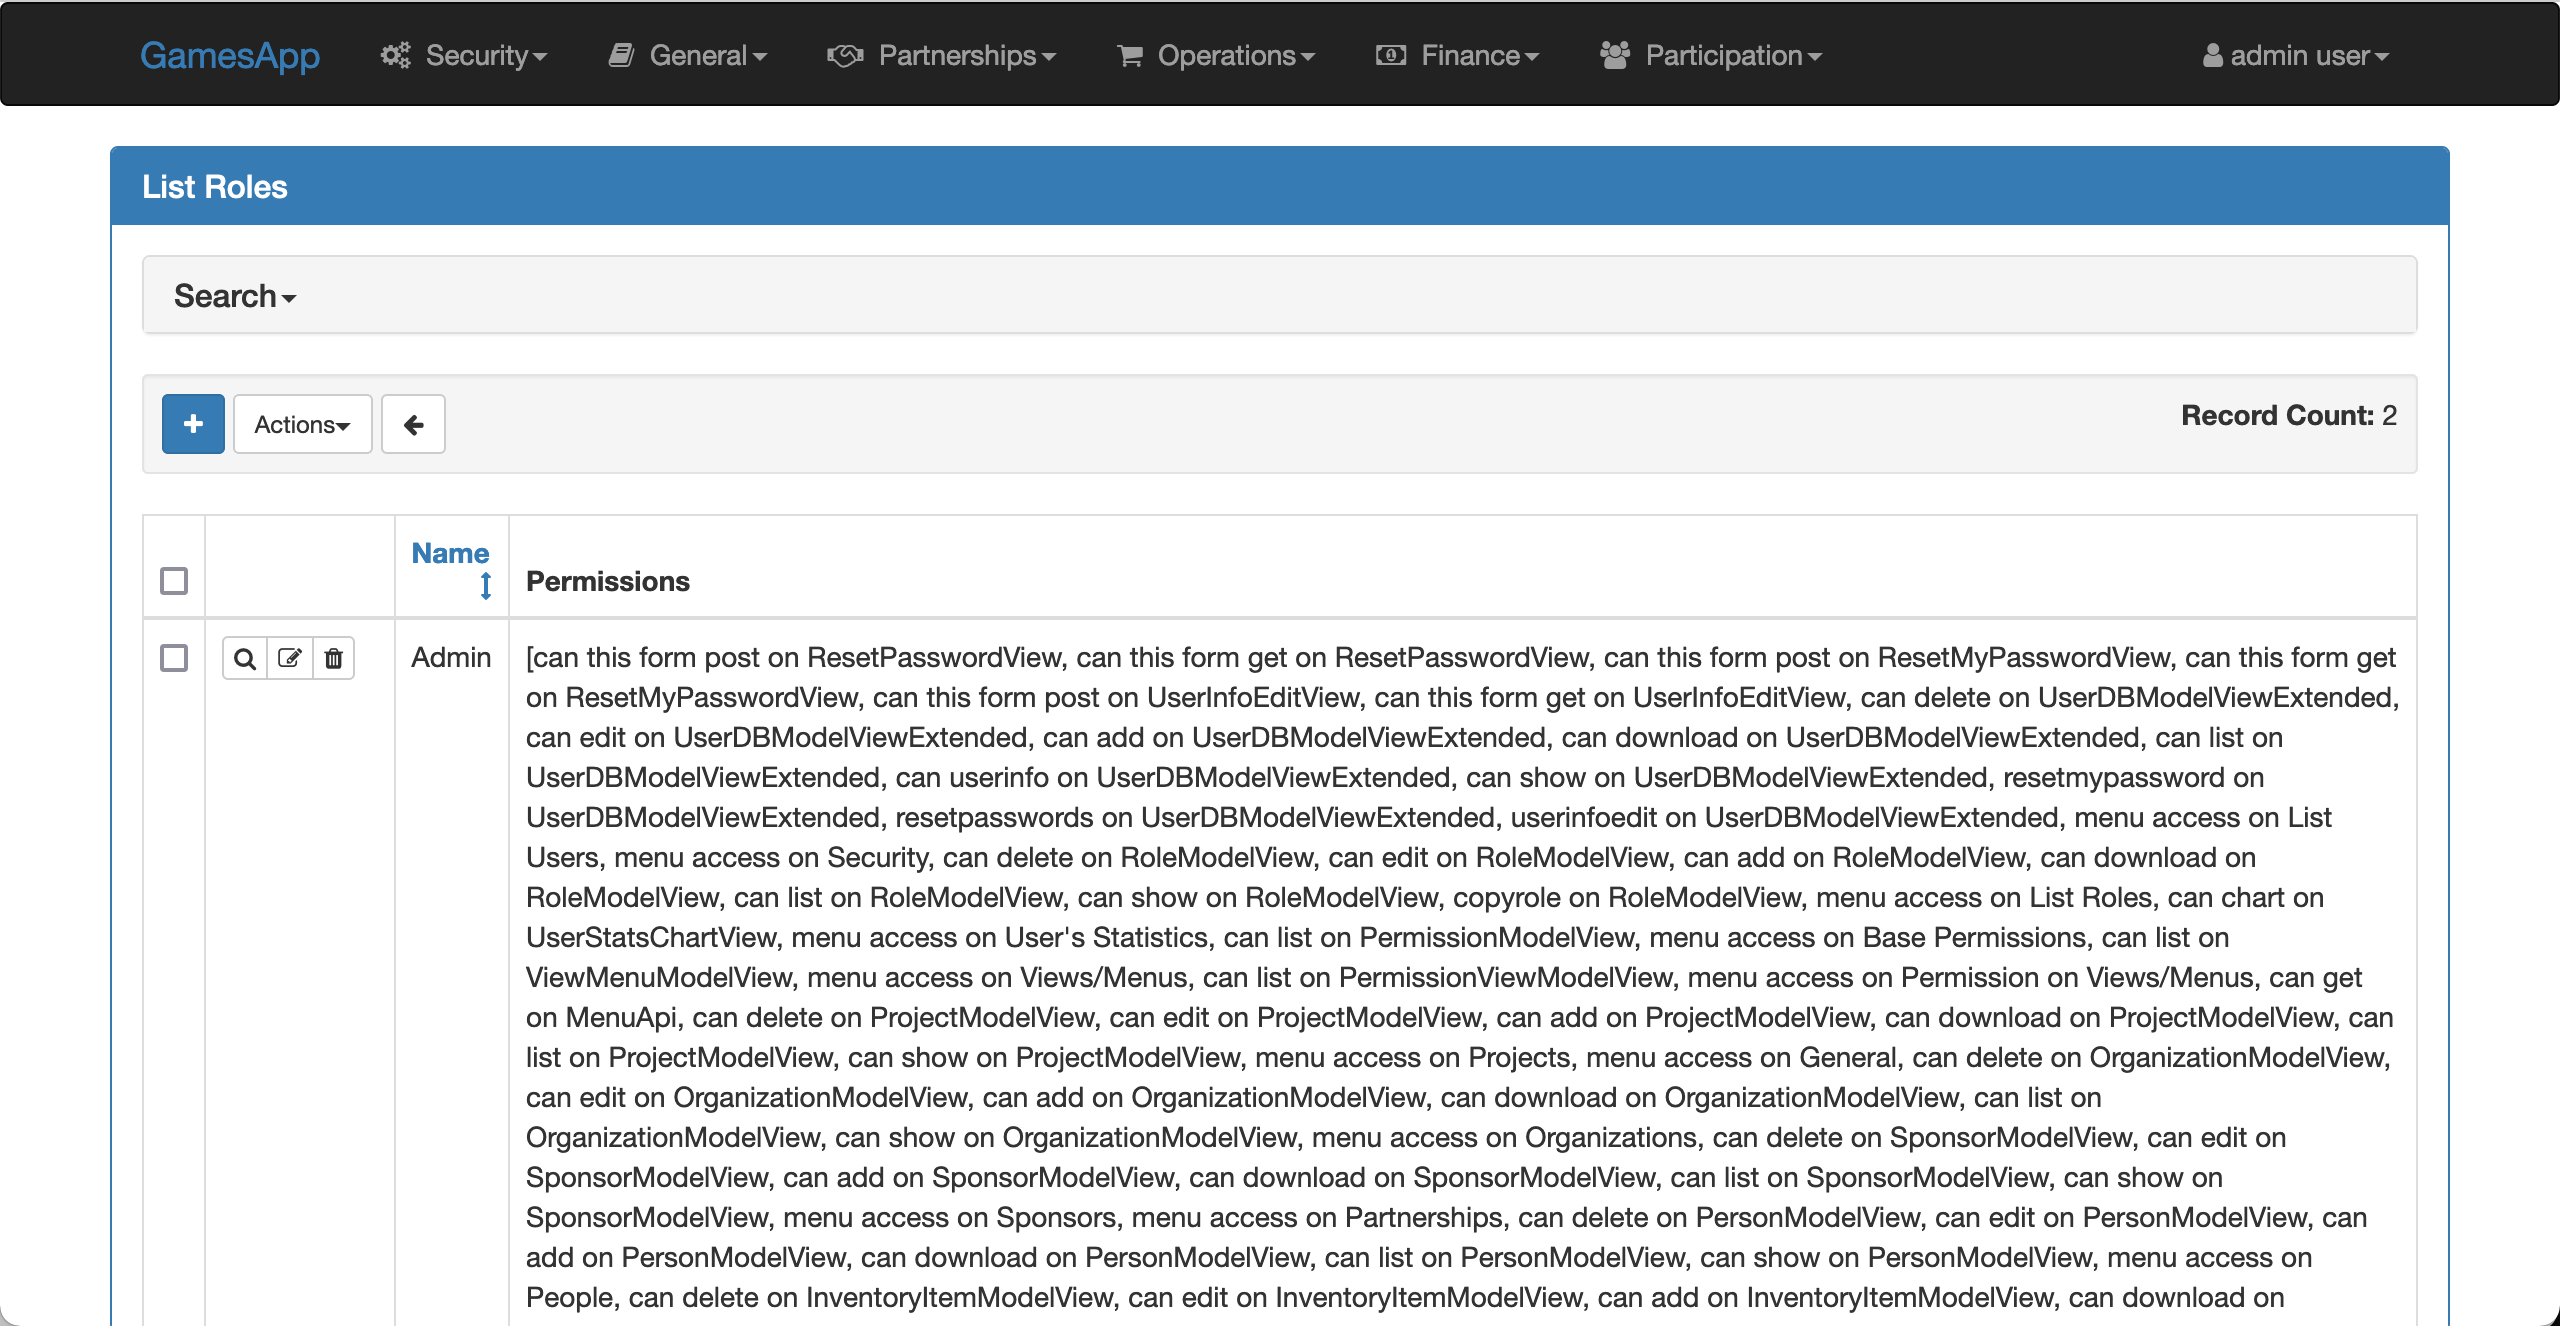
\includegraphics[width=1\textwidth]{slike/listroles.png}
    \caption{Prikaz \emph{List Roles}}
    \label{fig:listroles}
\end{figure}

Stvaranje nove uloge može se postići pritiskom na gumb označen znakom plus na
otvorenom prikazu. Potrebno je odabrati ime uloge te odgovarajuće dozvole u
sustavu koje toj ulozi pripadaju. Kao što se na slici \ref{fig:addrole} može
vidjeti, sučelje za odabir dozvola u paketu \emph{Flask-Appbuilder} izvedeno je
na izrazito nepraktičan način.

\begin{figure}[H]
    \centering
    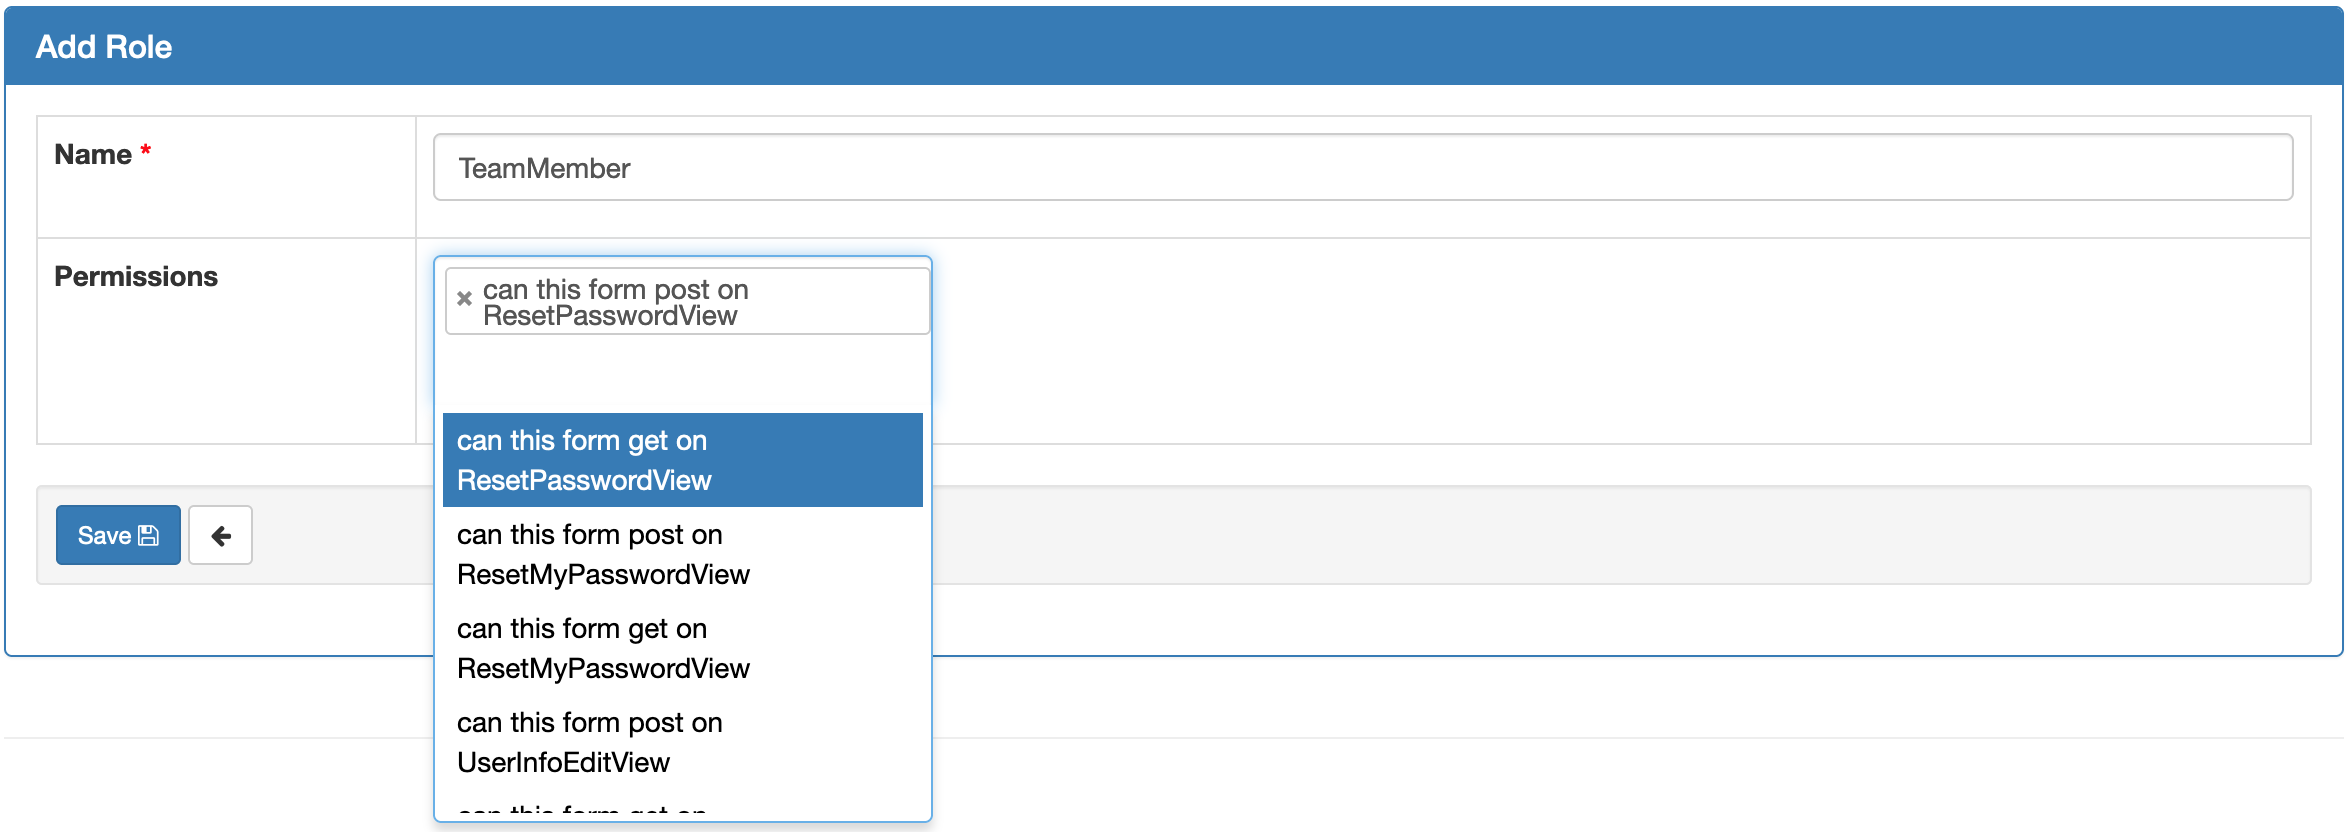
\includegraphics[width=1\textwidth]{slike/addrole.png}
    \caption{Dodavanje uloge}
    \label{fig:addrole}
\end{figure}

Administrator ili za to ovlašten korisnik potom može pregledavati, uređivati ili
dodavati korisnike odabirom opcije \emph{List Users}, također iz izbornika
\emph{Security}. Prilikom dodavanja korisnika, administrator odabire njegove
uloge, postavlja inicijalnu lozinku te eventualno povezuje korisnika sa zapisom
o osobi u bazi podataka. Korisnik će potom moći promijeniti svoju lozinku nakon
što se prijavi s onom inicijalno postavljenom.

\begin{figure}[H]
    \centering
    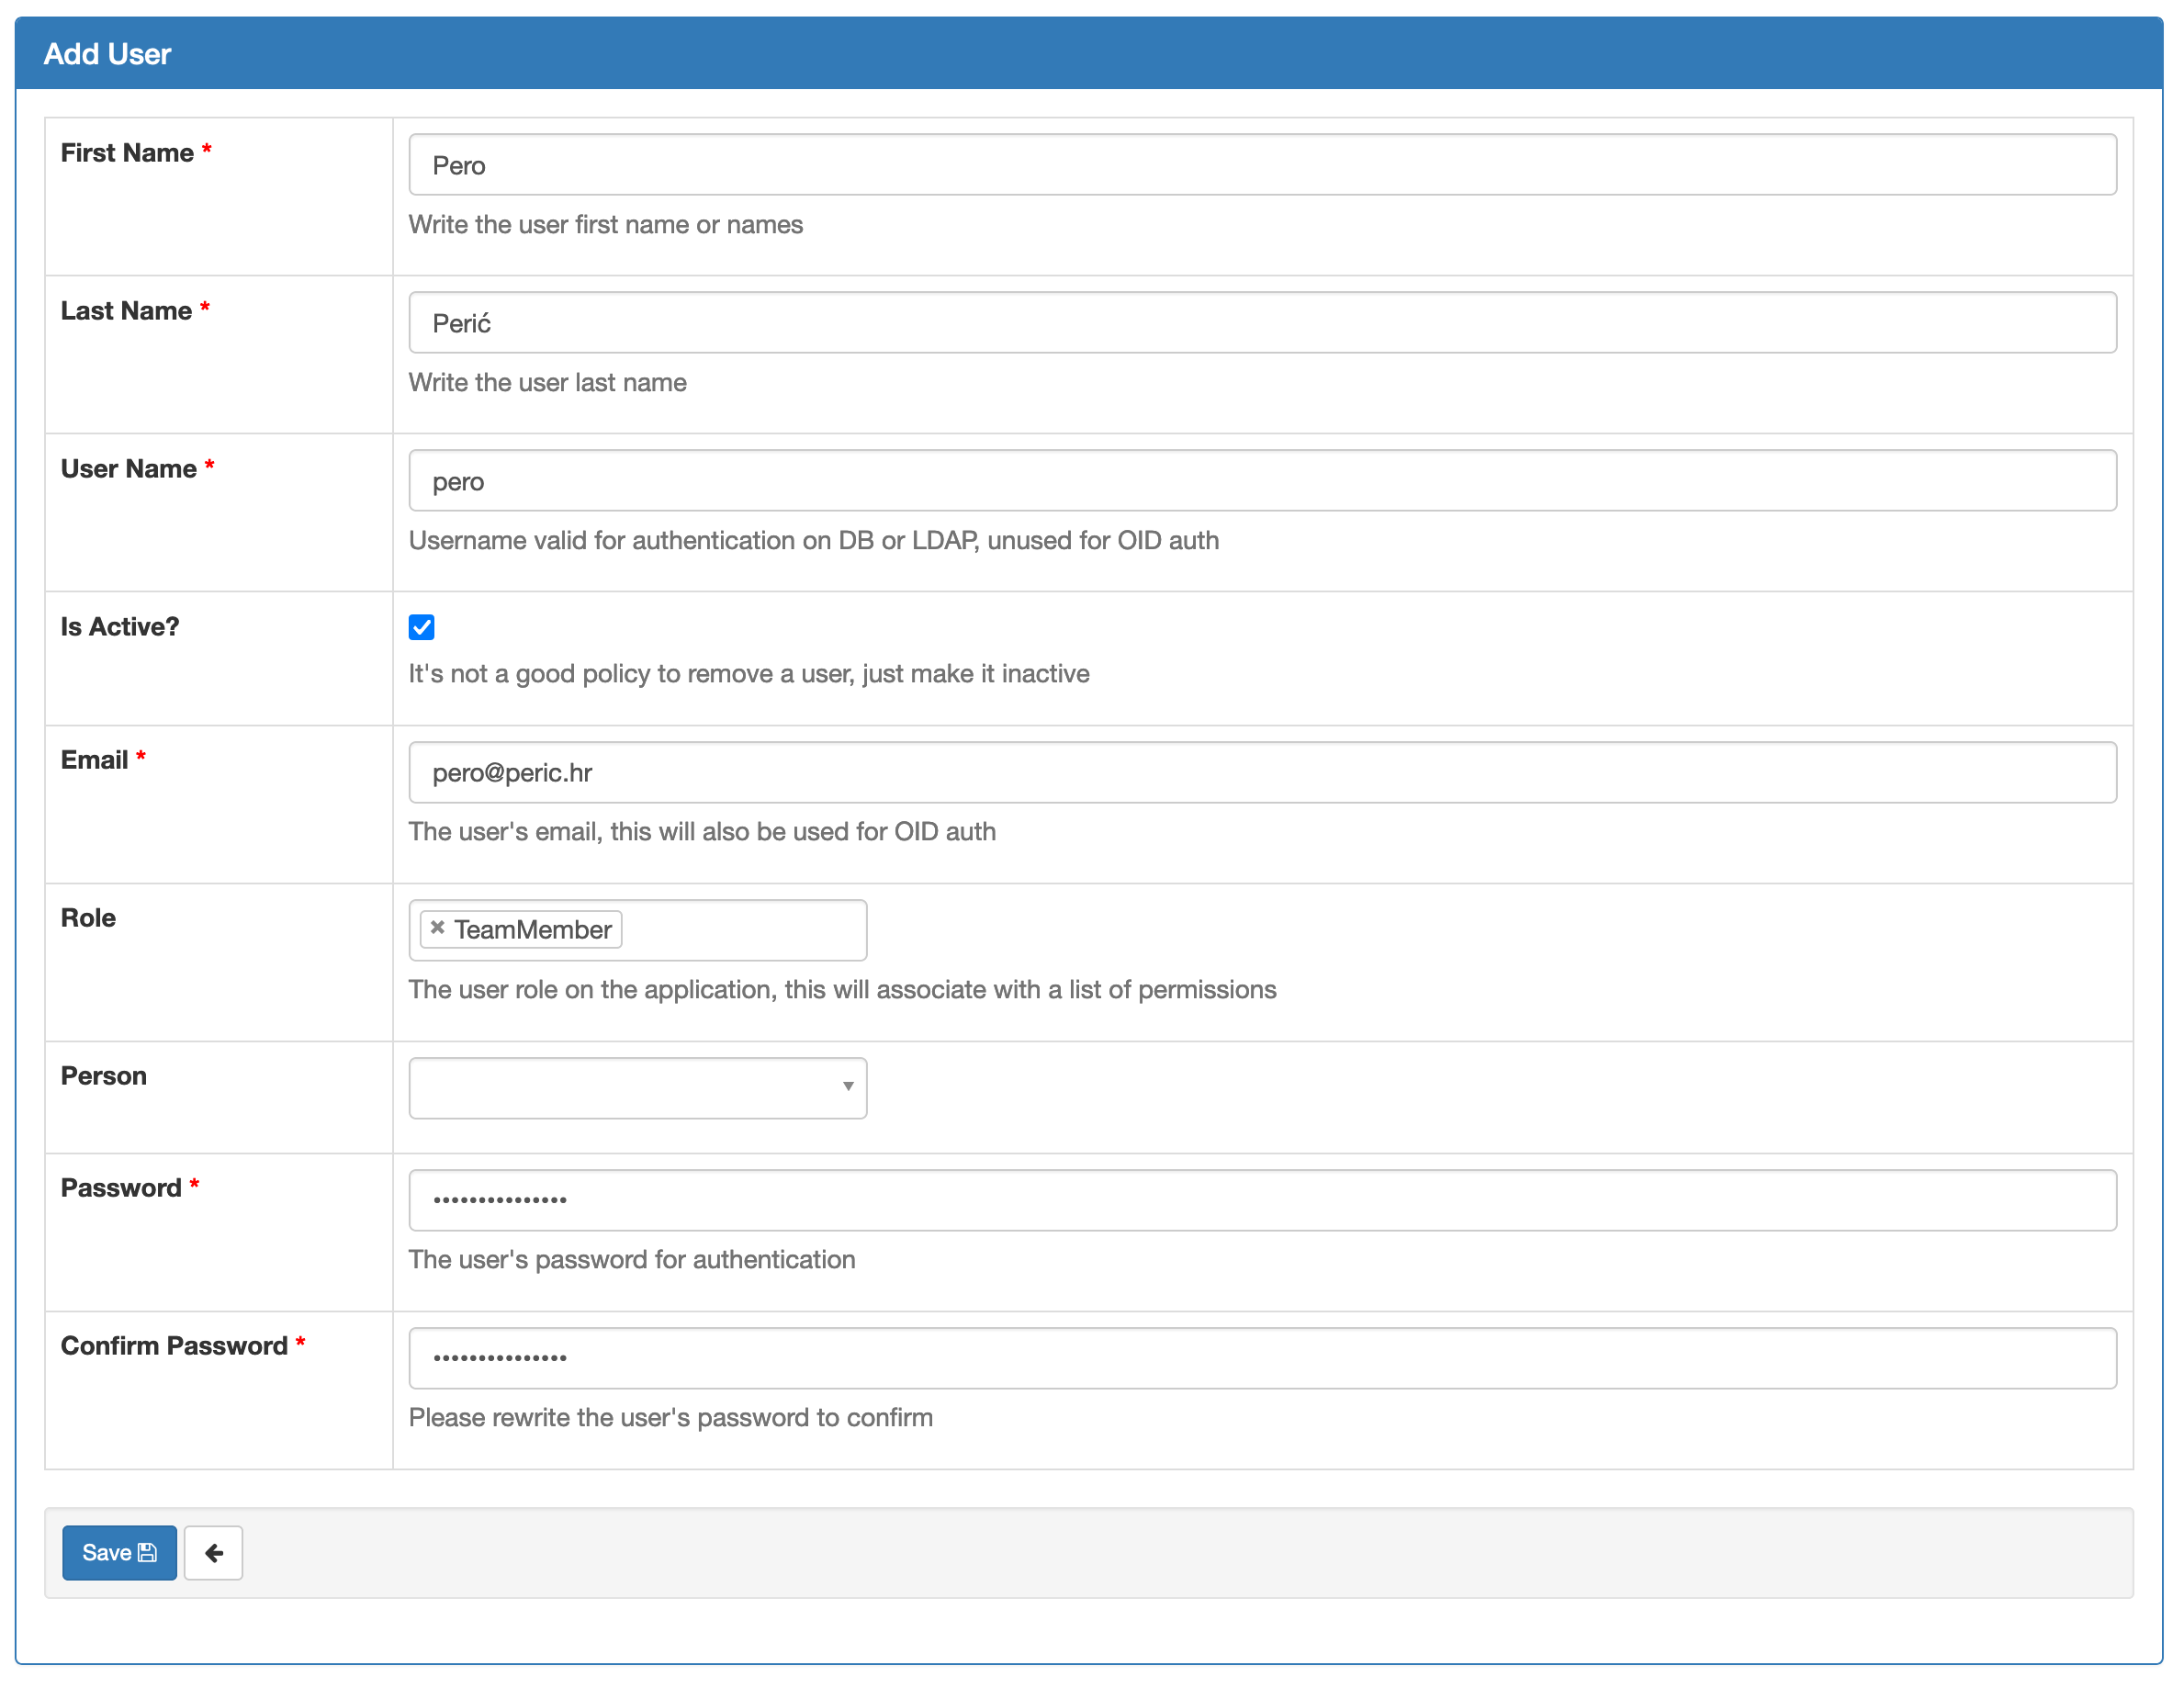
\includegraphics[width=1\textwidth]{slike/userform.png}
    \caption{Dodavanje korisnika}
    \label{fig:userform}
\end{figure}

Svaki korisnik može biti aktivan ili neaktivan. Sustav omogućuje i
predlaže administratoru da korisnike deaktivira umjesto brisanja.

\subsection{Upravljanje podacima}

Na primjeru dodavanja jednog sponzorstva bit će ilustrirano postupanje s podacima u
sustavu. Sučelje za upravljanje svim ostalim entitetima navedenim u poglavlju
\ref{model} funkcionira na identičan način.

Odabirom opcije \emph{Sponsors} iz izbornika \emph{Partnerships} otvara se popis
sponzorstava.

\begin{figure}[H]
    \centering
    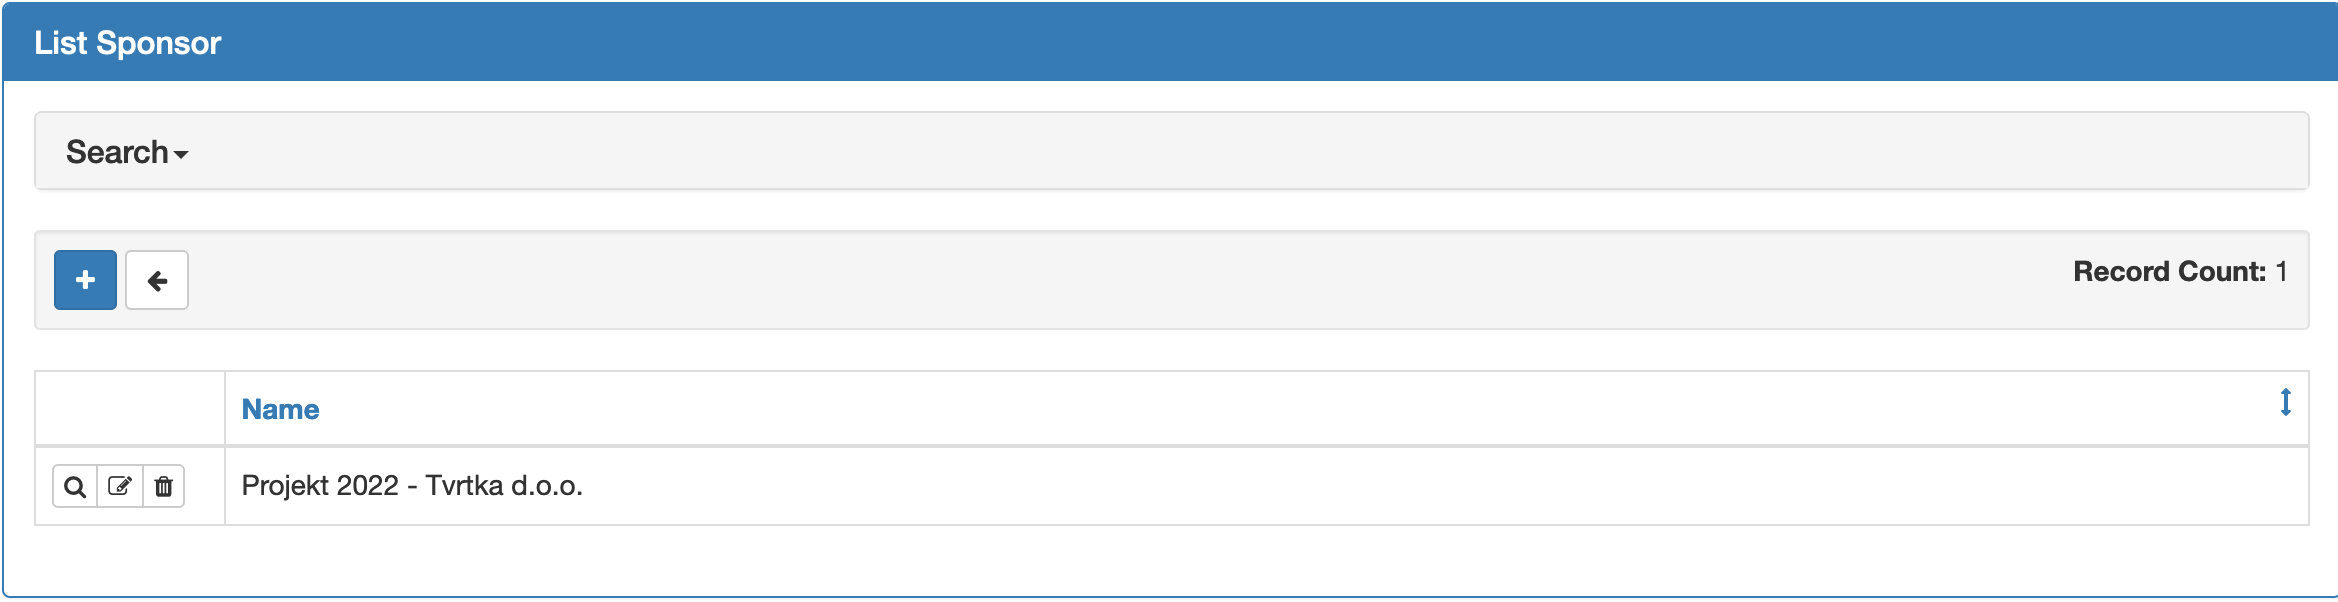
\includegraphics[width=1\textwidth]{slike/sponsormaster.png}
    \caption{Popis sponzorstava}
    \label{fig:listsponsors}
\end{figure}

Pritiskom na gumb označen znakom plus moguće je dodati novog sponzora.

\begin{figure}[H]
    \centering
    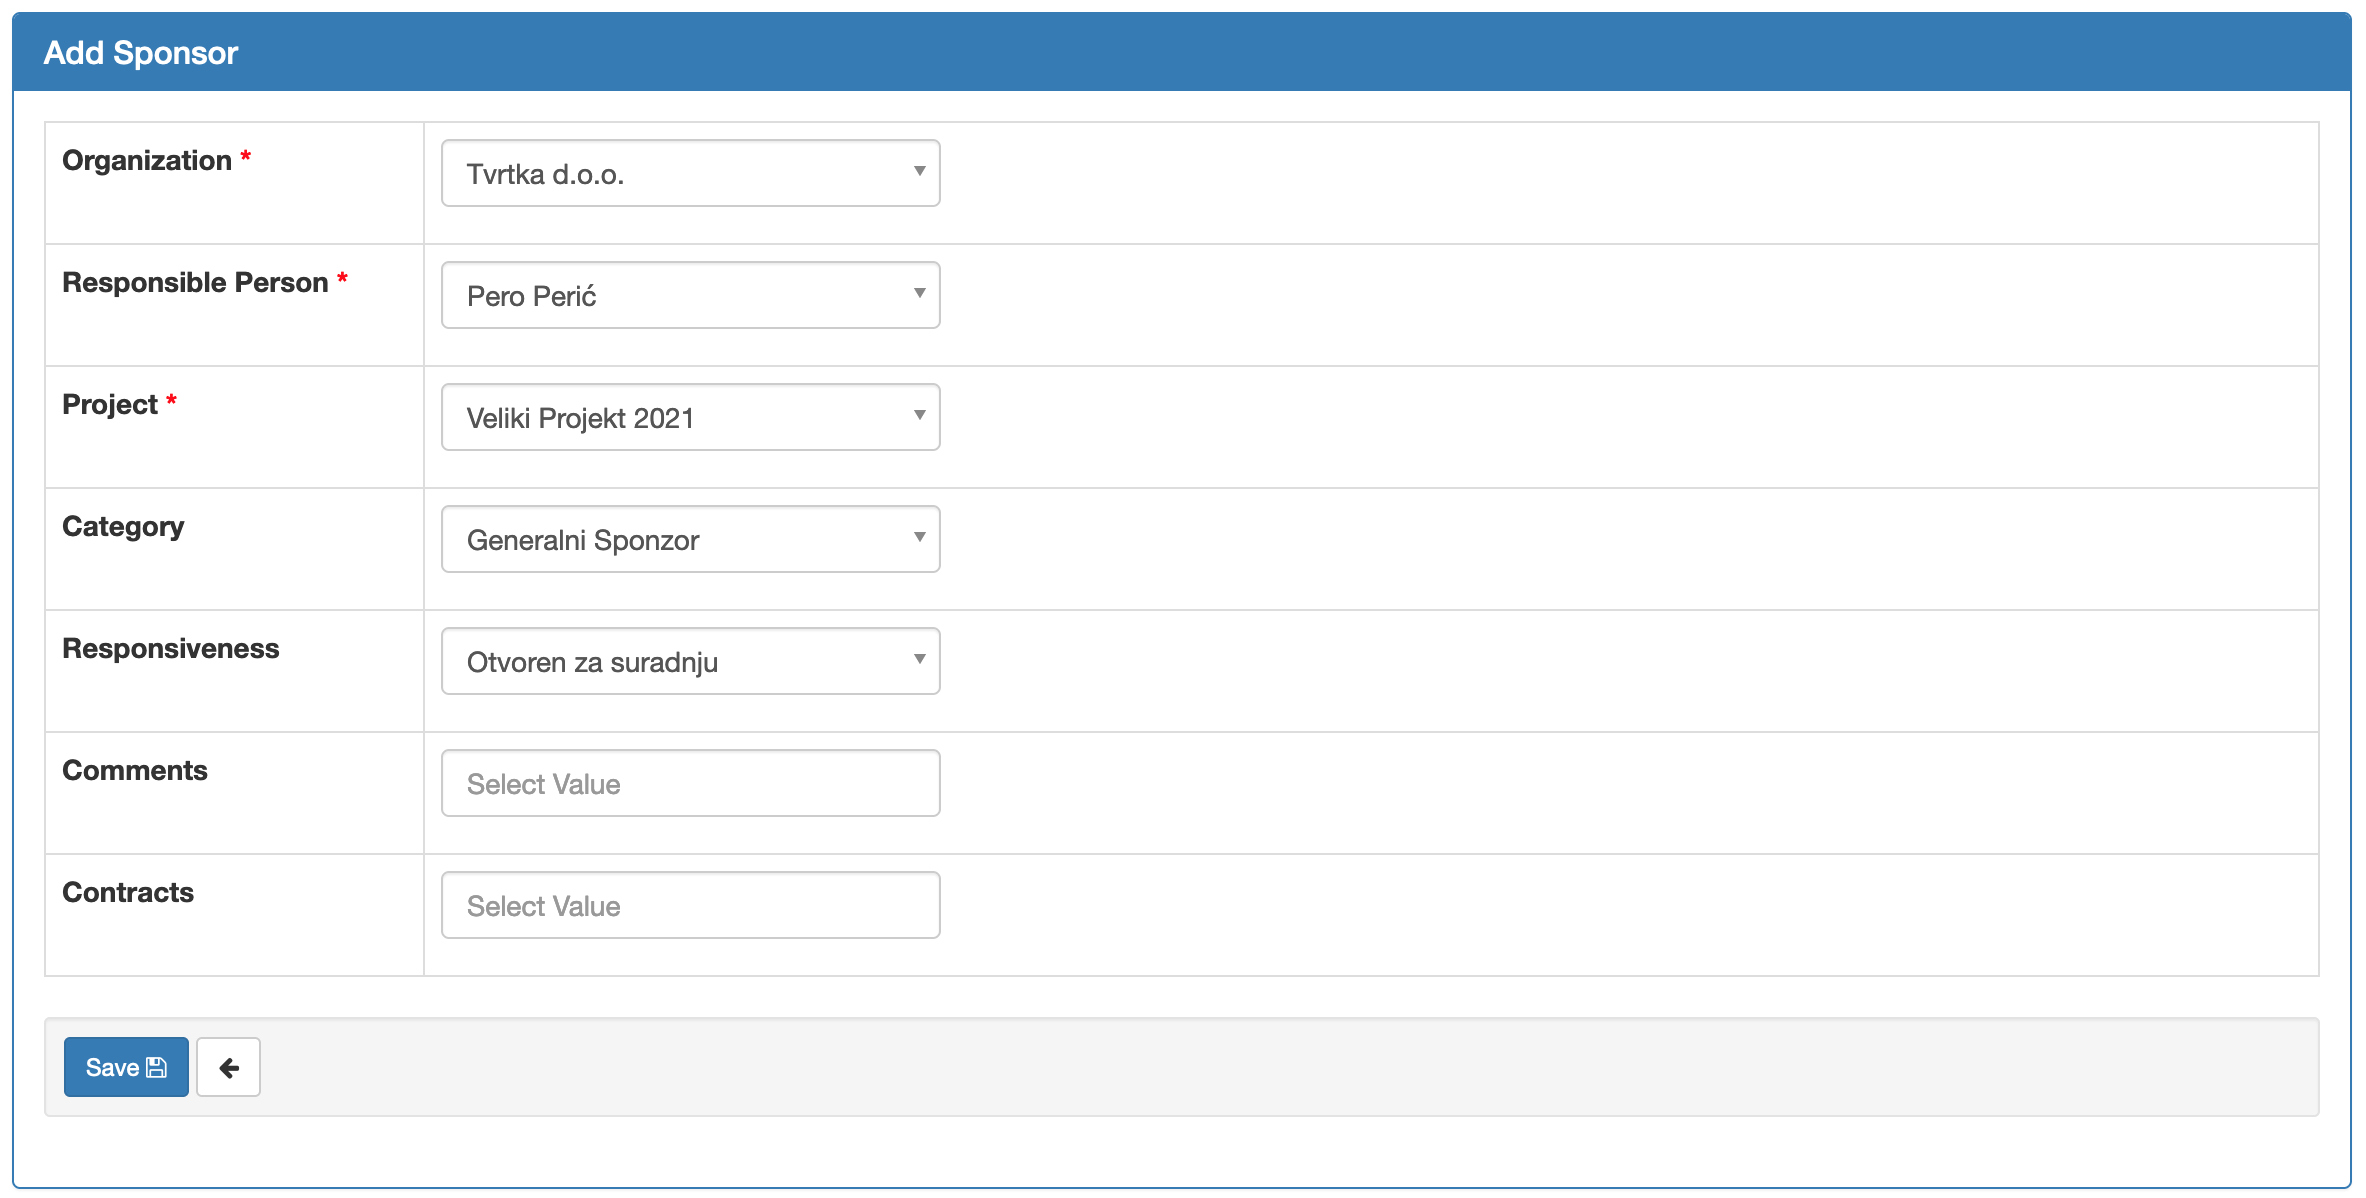
\includegraphics[width=1\textwidth]{slike/addsponsor.png}
    \caption{Dodavanje sponzora}
    \label{fig:addsponsor}
\end{figure}

Dodani sponzor potom će se pojaviti u glavnom prikazu.

\begin{figure}[H]
    \centering
    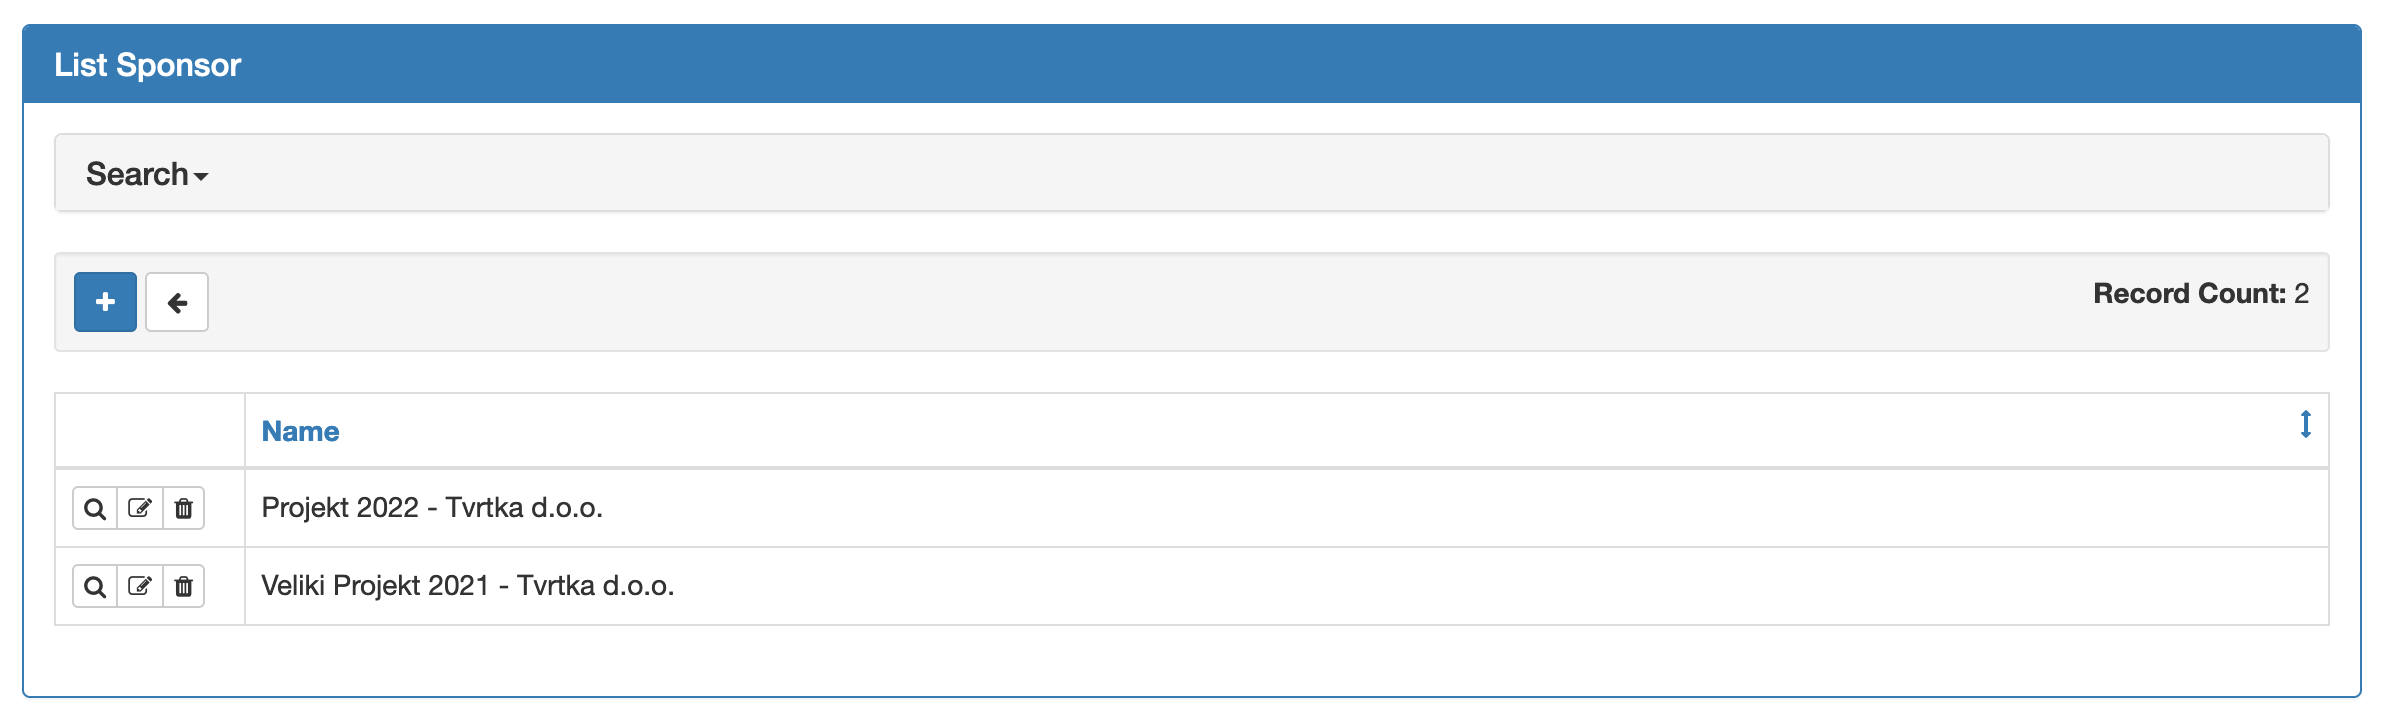
\includegraphics[width=1\textwidth]{slike/sponsoradded.png}
    \caption{Sponzor dodan na popis}
    \label{fig:sponsoradded}
\end{figure}

Podaci se potom mogu filtrirati dodavanjem filtra u okviru \emph{Search}.

\begin{figure}[H]
    \centering
    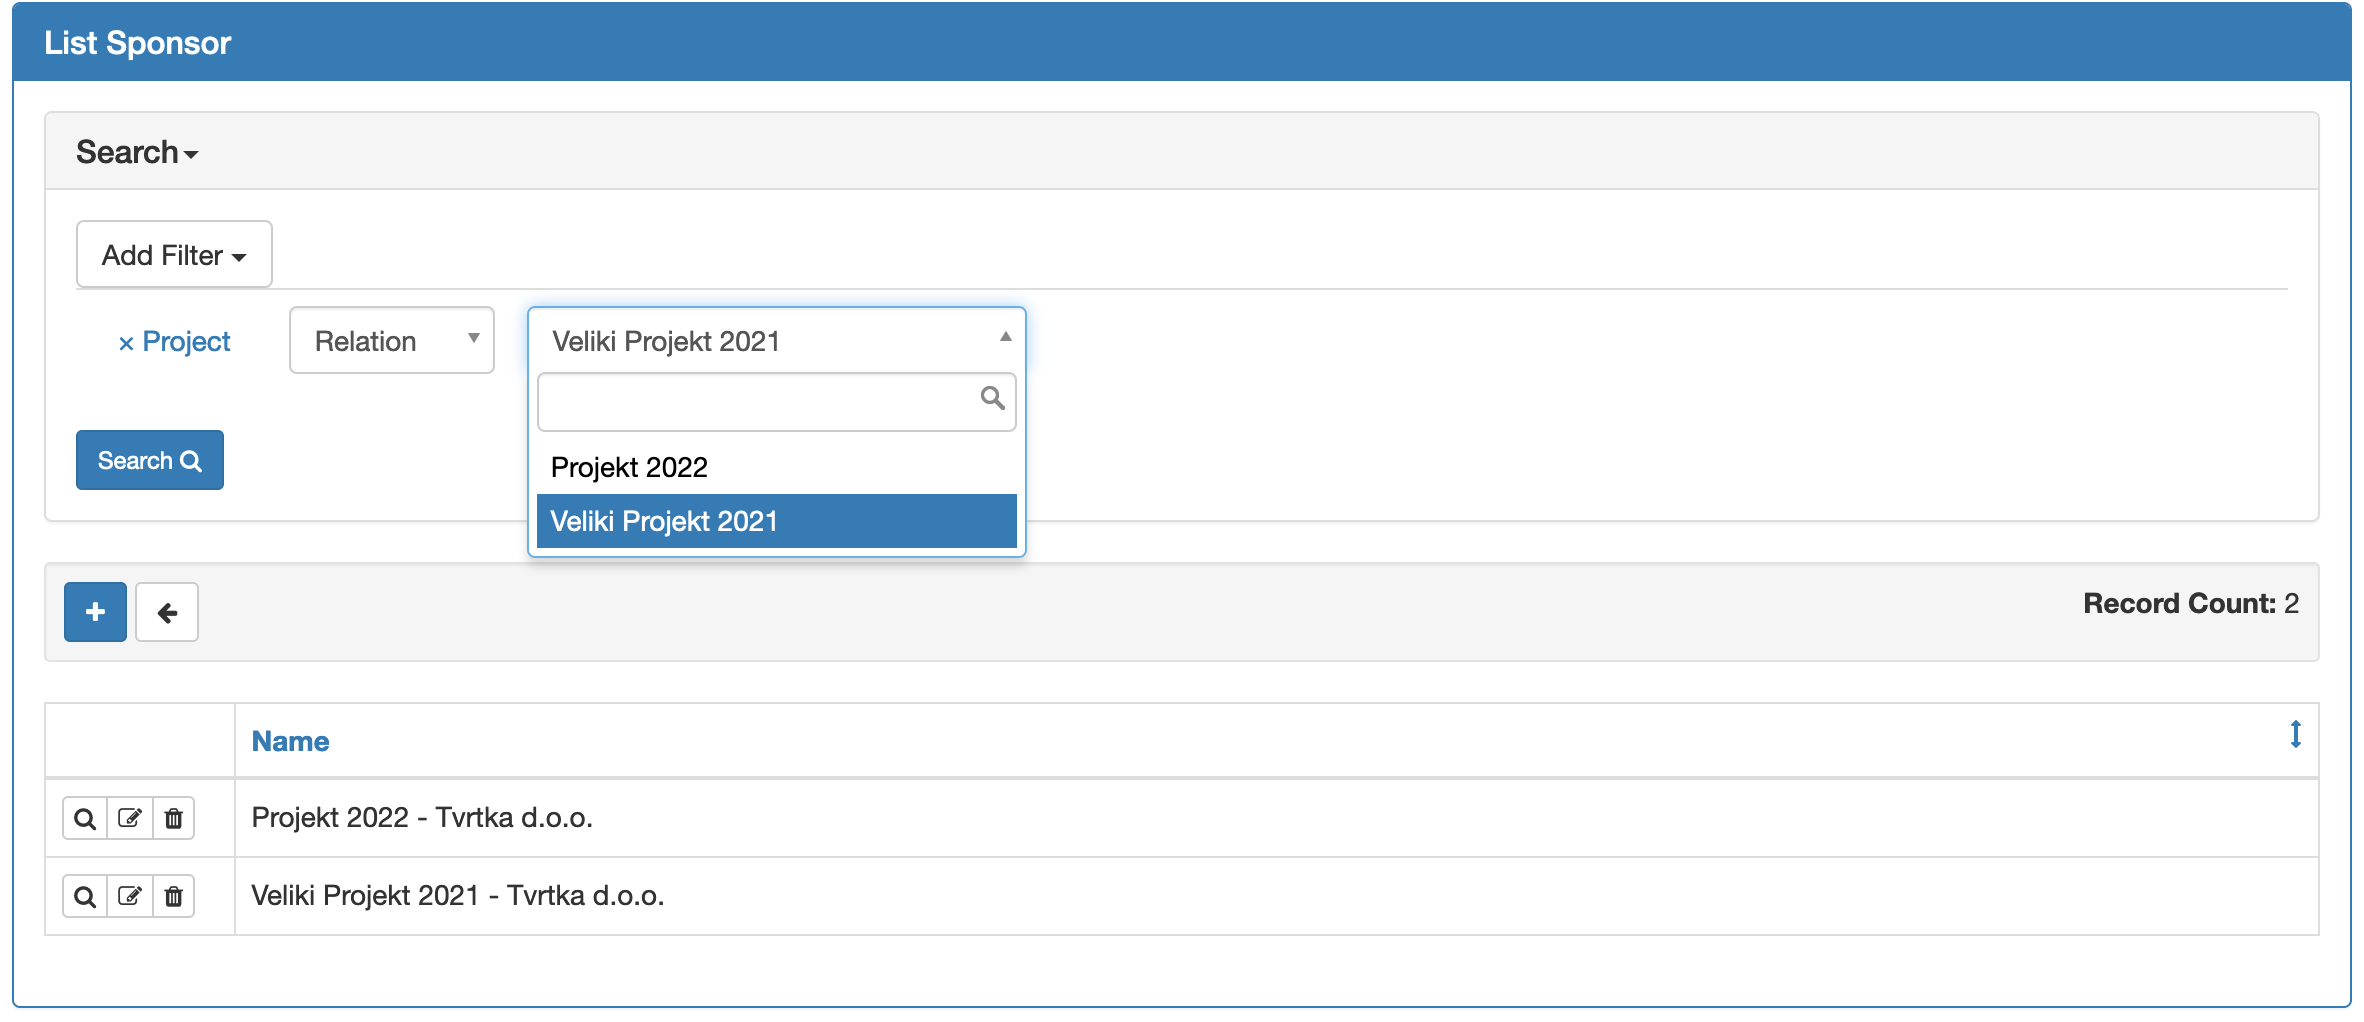
\includegraphics[width=1\textwidth]{slike/sponsorfilter.png}
    \caption{Definiranje filtra}
    \label{fig:sponsorfilter}
\end{figure}

Pritiskom na gumb označen ikonom povećala pokraj zapisa u glavnom prikazu otvara
se detaljni prikaz zapisa u kojem su dostupni i povezani prikazi (u ovom slučaju
prikaz koji se odnosi na komentare o sponzoru).

\begin{figure}[H]
    \centering
    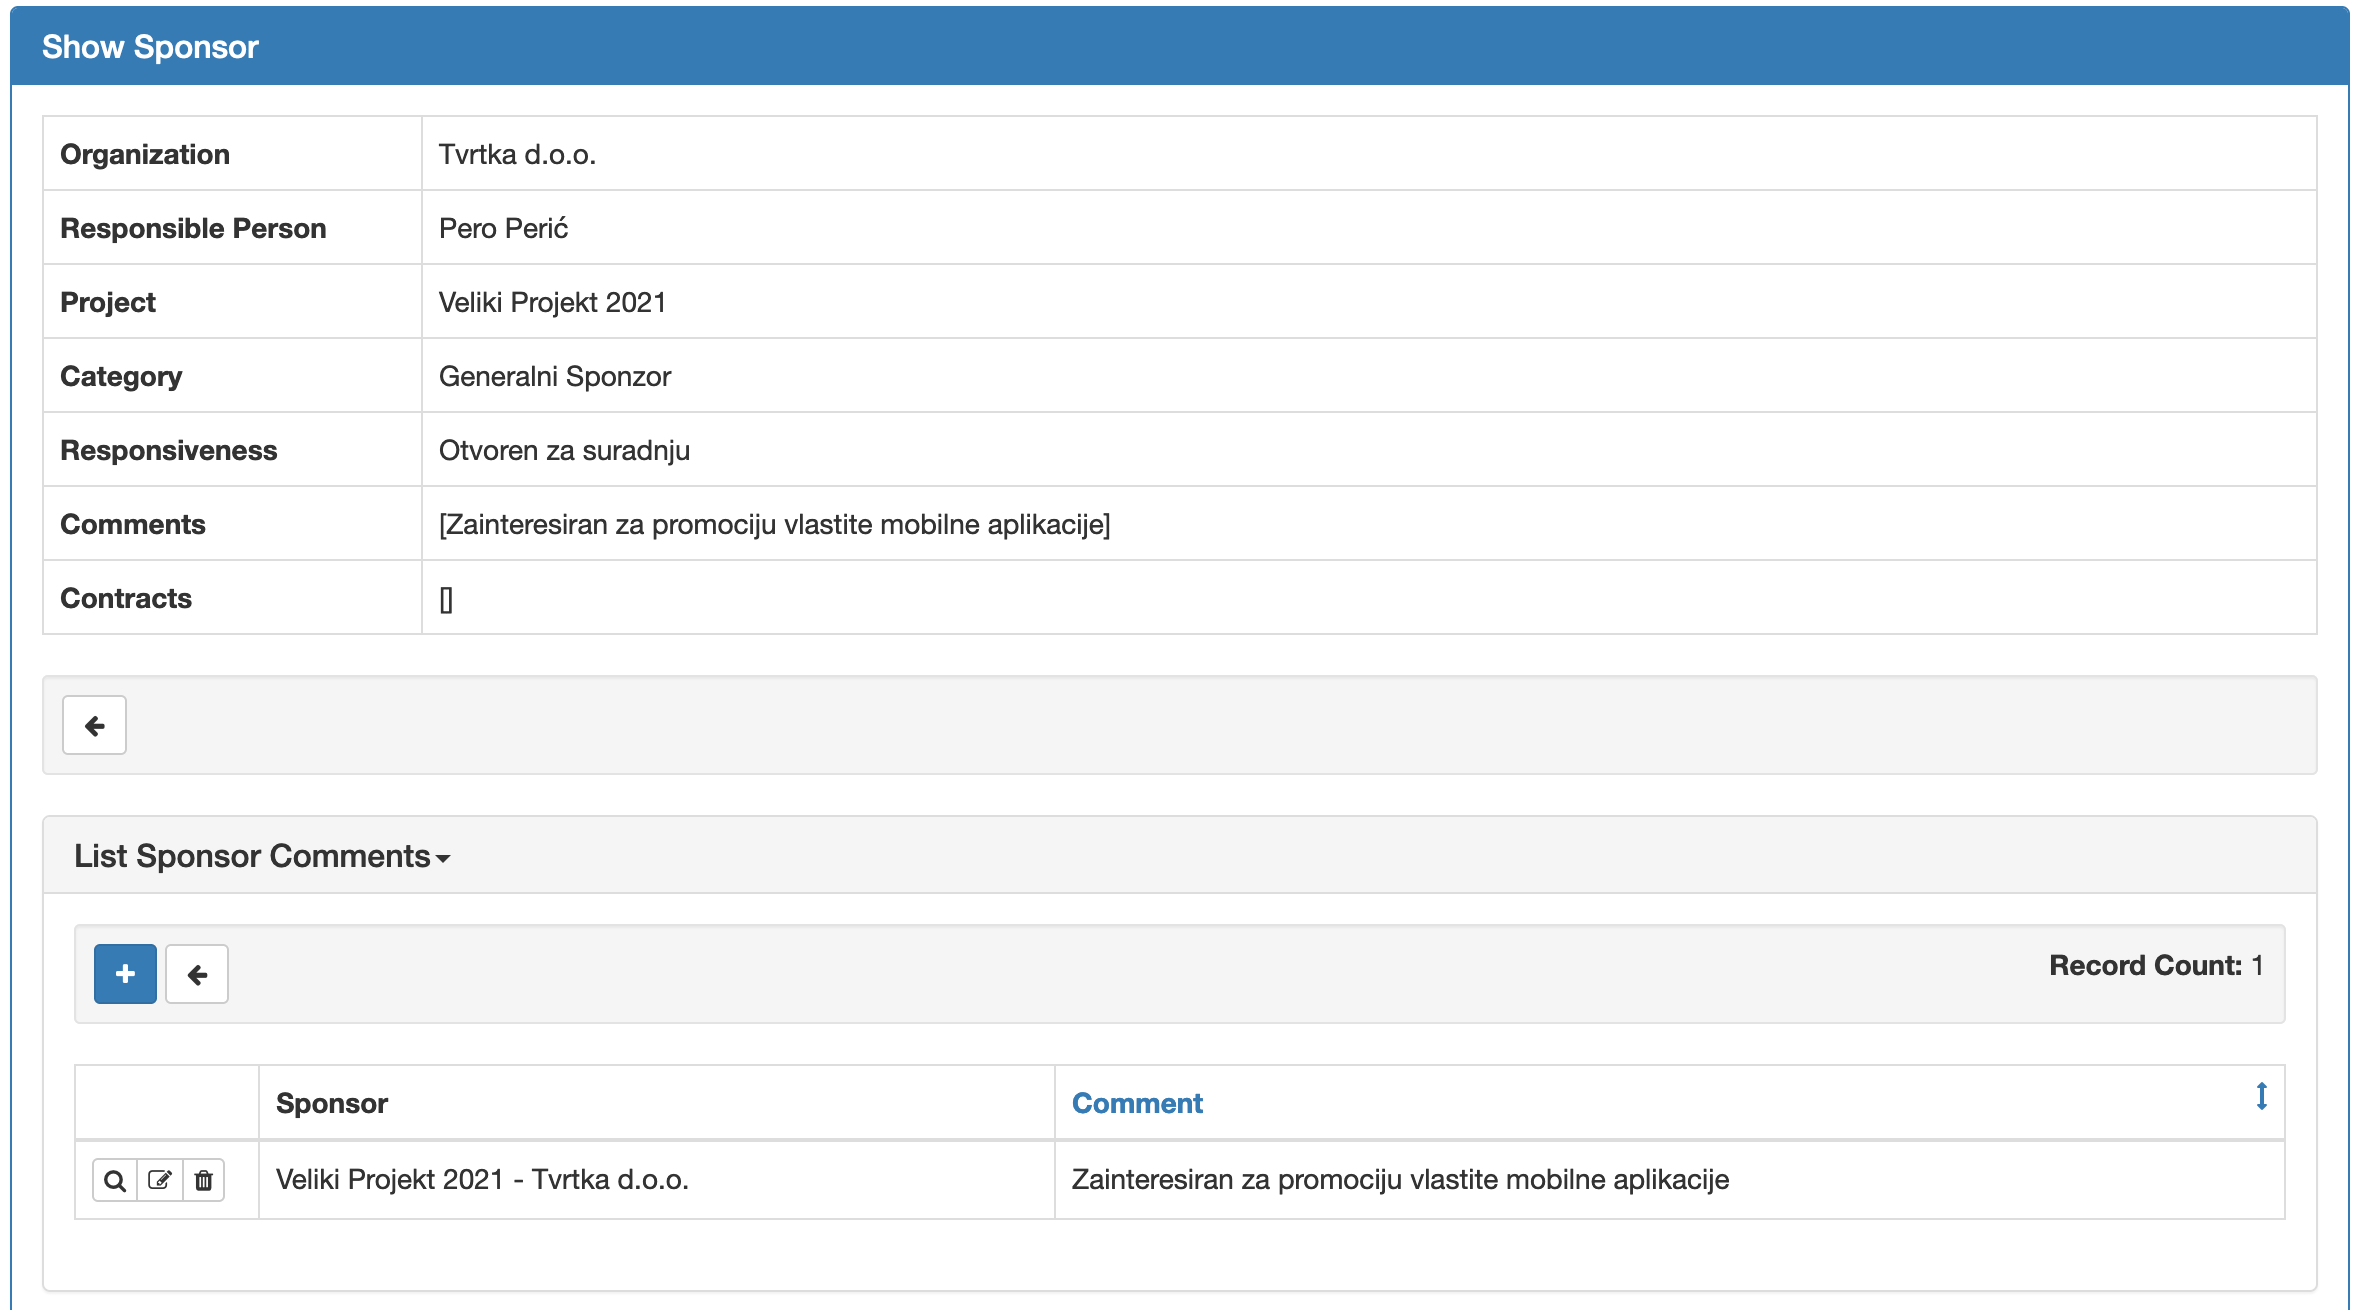
\includegraphics[width=1\textwidth]{slike/detail.png}
    \caption{Detaljni prikaz zapisa o sponzoru}
    \label{fig:detail}
\end{figure}

Podatak o sponzoru sada je također dostupan u detaljnom pregledu projekta pod
odgovarajućom karticom.

\begin{figure}[H]
    \centering
    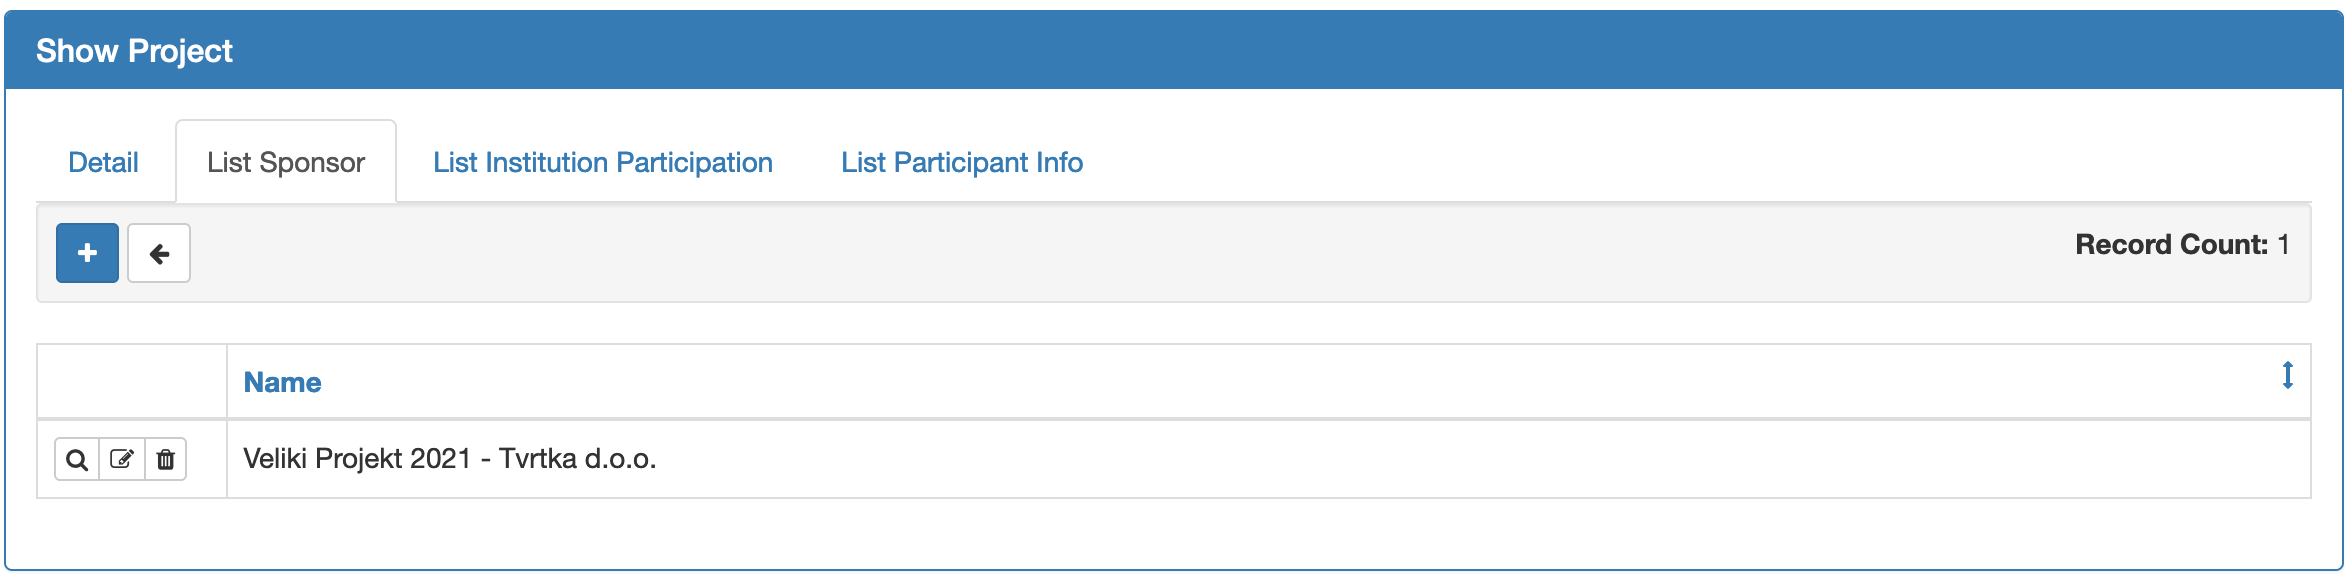
\includegraphics[width=1\textwidth]{slike/projectsponsor.png}
    \caption{Pregled sponzora projekta u detaljnom prikazu projekta}
    \label{fig:projectsponsor}
\end{figure}

Uz svaki zapis u tabličnim prikazima dostupni su i gumbi za uređivanje i
brisanje zapisa. Prava na svaku od ovih operacija uređena su pojedinačnim,
automatski generiranim dozvolama u sustavu.

\section{Nedostaci i prostor za nadogradnju}

Ovakav pristup u razvoju aplikacije pokazao se jednostavan i brz te autor
vjeruje da uz pomoć ovog rada aplikaciju mogu nadograđivati i osobe slabije
tehničke pozadine. Ipak, mogućnosti aplikacije razvijene na ovaj način
ograničene su na funkcionalnosti koje nudi \emph{RAD} programski paket -- bilo
kakvu napredniju nadogradnju potrebno je razviti na tradicionalan način.

Glavna ograničenja primijećena u razvoju aplikacije odnose se na nedostatak
mogućnosti za preuzimanjem podataka u tabličnom obliku te nemogućnost
agregiranja podataka (računanja zbrojeva, prosjeka i slično). U budućnosti bi
bilo korisno nadograditi funkcionalnost korištenog programskog paketa kako bi se
nadomjestila spomenuta ograničenja.

Već spomenuto ograničenje također je upravljanje dozvolama koje je u programskom
paketu izvedeno na nepraktičan način. Bolje rješenje s aspekta korisničkog
sučelja moglo bi se postići organizacijom dozvola u stablastu strukturu te
omogućavanjem dodjele grupa dozvola, no takva nadogradnja zahtijevala bi promjenu
podatkovnog modela i izradu nove vrste obrasca.

S obzirom na to da je razvijeni sustav \emph{Flask} aplikacija, te da koristi
uvriježenu \emph{SQLAlchemy} knjižnicu, nadogradnje na sustav mogu se razvijati
na tradicionalan način u okvirima koje pruža \emph{Flask} paket neovisno o
paradigmi paketa \emph{Flask-Appbuilder}. Razvoj takvih nadogradnji, ipak,
zahtjeva više resursa i znanja nego razvoj aplikacije uz ovakav \emph{low-code}
pristup te stoga nije uvijek u mogućnostima jedne studentske organizacije.

Dodatna zapreka pri korištenju konkretnog \emph{Flask-Appbuilder} paketa, već
spomenuta u potpoglavlju \ref{acc_ctr}, jest loša dokumentacija paketa. Većina
razreda i funkcija koje paket definira nisu opisane u njegovoj dokumentaciji te
se ponekad treba referirati na kod paketa što bi volonteru s manje tehničkih
znanja moglo predstavljati problem. Ipak, većina potrebnih osnovnih
funkcionalnosti opisana je u dokumentaciji.

Razvijenom aplikacijom također nisu pokriveni svi zahtjevi navedeni u poglavlju
\ref{reqs} jer bi time aplikacija prešla opseg ovog rada. Zahtjevi za
implementaciju odabrani su prema subjektivnoj procjeni prioriteta proizašloj iz
iskustva rada u organizaciji i razgovora s volonterima. Cilj ovog rada među
ostalim je dokumentirati postupak razvoja aplikacije kako bi se omogućila
buduća nadogradnja ukoliko se za tim pokaže potreba.

\chapter{Zaključak}

U sklopu ovog diplomskog rada razmotren je rad jedne studentske organizacije
koja organizira natjecanje s velikim brojem sudionika na primjeru
\emph{Organizacije za studentska natjecanja STEM Games} te su iz opisa njezinog
djelovanja izdvojeni najvažniji zahtjevi na informacijski sustav za podršku radu
organizacije. Potom je ukratko promotrena primjenjivost \emph{ERP} rješenja
otvorenog koda u odnosu na navedene zahtjeve. Naposljetku, razvijen je i
dokumentiran informacijski sustav oblikovan prema zahtjevima organizacije i
implementiran pomoću \emph{RAD} programskog okvira \emph{Flask-Appbuilder}.

U evaluaciji oba pristupa pokazalo se da \emph{ERP} rješenje ne pokriva dio
zahtjeva koji su specifični za studentsku organizaciju ovog tipa, dok s druge
strane nudi mnoge nepotrebne mogućnosti koje povećavaju kompleksnost njegove
uporabe. Područje u kojemu je \emph{ERP} rješenje u velikoj prednosti jest
vođenje financija udruge, s obzirom na to da se mogućnosti koje nudi ne mogu
implementirati koristeći \emph{RAD} programski okvir.

U drugim aspektima, aplikacija razvijena pomoću \emph{RAD} programskog okvira
adekvatna je i pokriva većinu organizacijskih potreba koje se svode na pohranu
podataka. Proces razvoja pokazao se jednostavnim te se iz razgovora s
volonterima u organizaciji dalo zaključiti da je nadogradnja razvijene
aplikacije unutar mogućnosti studenta volontera. Jedan od ciljeva ovog rada bio
je i olakšati takve eventualne nadogradnje dokumentirajući postupak razvoja.

Nakon predstavljanja razvijene aplikacije, voditelji timova \emph{Udruge}
iskazali su podršku uvođenju ovakvog sustava. Primijećen je nedostatak
funkcionalnosti oko financijskog aspekta aplikacije, što dovodi do zaključka da
pristup razvoju korišten u ovom radu ne može u potpunosti ispuniti zahtjeve
vezane uz financije \emph{Udruge}. Taj bi se nedostatak mogao nadomjestiti
nadogradnjom razvijenom na klasičan način, no s obzirom na adekvatnost
\emph{ERP} modula u tom aspektu valjalo bi razmotriti korištenje isključivo toga
modula paralelno uz razvijenu aplikaciju.

Primjenjivost razvijenog sustava te praktičnost njegove nadogradnje konačno će
se pokazati kroz njegovo korištenje u praksi na budućim projektima
\emph{Udruge}.

\bibliography{literatura}
\bibliographystyle{fer}

\appendix
\chapter{Struktura direktorija razvijene aplikacije}
\begin{lstlisting}[basicstyle=\footnotesize,frame=single]
README.rst
__pycache__
app
app.db
babel
config.py
run.py

./app:
__init__.py
__pycache__
index.py
models.py
models.py.html
models_for_print.html
sec.py
sec_views.py
templates
translations
views.py

./app/templates:
404.html
my_index.html

./app/translations:
pt

./app/translations/pt:
LC_MESSAGES

./app/translations/pt/LC_MESSAGES:
messages.mo
messages.po

./babel:
babel.cfg
messages.pot
\end{lstlisting}

\chapter{Izbornici u razvijenoj aplikaciji}

\begin{figure}[H]
    \centering
    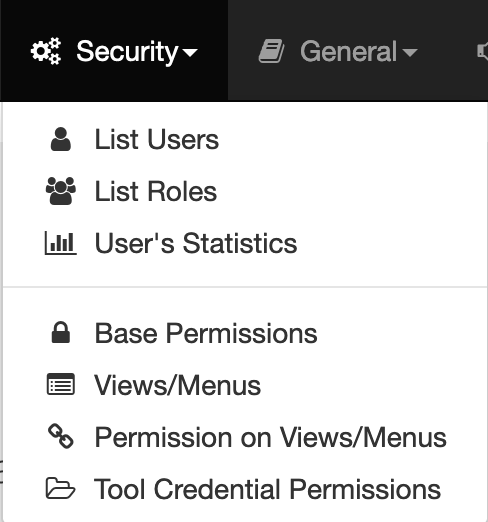
\includegraphics[width=0.4\textwidth]{slike/m0.png}
    \caption{Izbornik \emph{Security}}
\end{figure}
\begin{figure}[H]
    \centering
    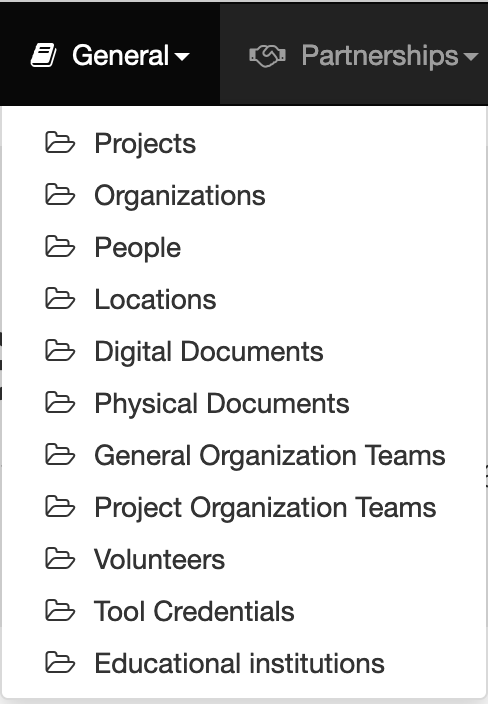
\includegraphics[width=0.4\textwidth]{slike/m1.png}
    \caption{Izbornik \emph{General}}
\end{figure}
\begin{figure}[H]
    \centering
    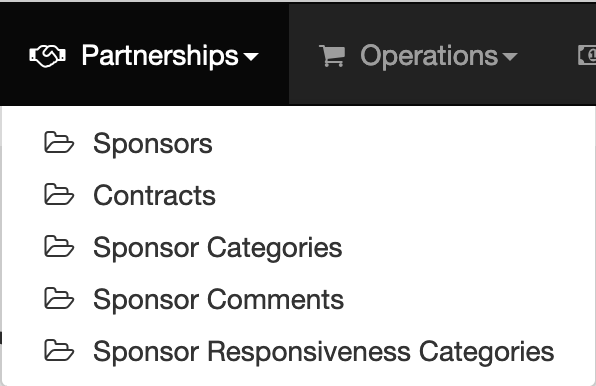
\includegraphics[width=0.4\textwidth]{slike/m2.png}
    \caption{Izbornik \emph{Partnerships}}
\end{figure}
\begin{figure}[H]
    \centering
    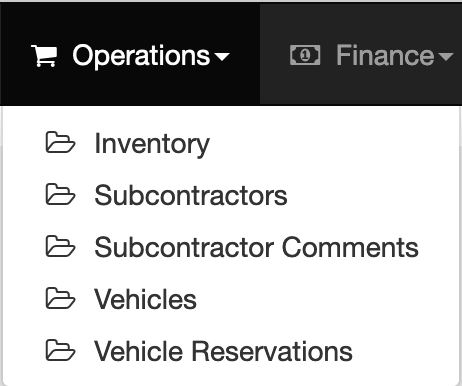
\includegraphics[width=0.4\textwidth]{slike/m3.png}
    \caption{Izbornik \emph{Operations}}
\end{figure}
\begin{figure}[H]
    \centering
    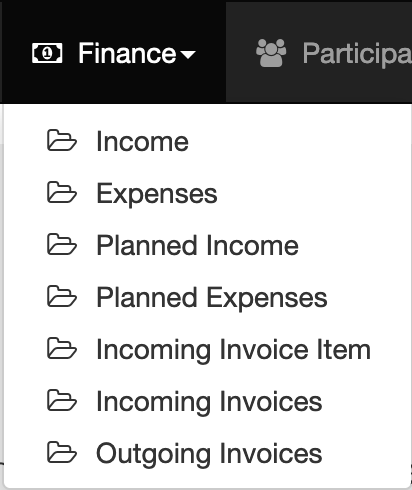
\includegraphics[width=0.4\textwidth]{slike/m4.png}
    \caption{Izbornik \emph{Finance}}
\end{figure}
\begin{figure}[H]
    \centering
    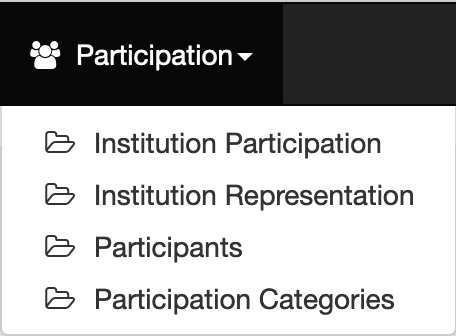
\includegraphics[width=0.4\textwidth]{slike/m5.png}
    \caption{Izbornik \emph{Participation}}
\end{figure}

\begin{sazetak}
Ovaj rad proučava pristup u implementaciji informacijskog sustava za potporu
studentskoj neprofitnoj udruzi koja organizira studentska natjecanja s velikim
brojem sudionika. Udruga tog tipa nema resursa za razvoj kompleksnog
informacijskog sustava, pa su stoga promotreni nezahtjevni pristupi za njegovo
ostvarenje. Zahtjevi na takav sustav proučeni su na primjeru Udruge za
studentska natjecanja STEM Games te su prema njima razmotreni pristupi korištenja gotovog
ERP rješenja te razvoja sustava koristeći Flask-Appbuilder programski
okvir za ubrzani razvoj aplikacija (RAD). Razvijen je informacijski sustav za navedenu
udrugu te je dokumentiran postupak razvoja. Pokazalo se da ERP sustav uvodi
nepotrebnu složenost i ne pokriva zahtjeve specifične za studentsku organizaciju
te da se korištenjem RAD okvira može brzo i lako razviti ograničen informacijski
sustav koji zadovoljava specifične potrebe organizacije.

\kljucnerijeci{RAD,studentska organizacija,ERP,informacijski sustav}
\end{sazetak}

\pagebreak

\engtitle{Development of an Information System to Facilitate the Organization of Large-Scale Events Using a Rapid Application Development Framework}
\begin{abstract}

This thesis studies approaches in implementing an information system to support
a student non-profit association that organizes large-scale student
competitions. Such an association lacks the necessary resources for the
development of a complex information system, so the analysis focuses on
non-demanding approaches of implementation. The requirements for such a system
are studied on the example of the Association for Student Competitions STEM
Games and are subsequently used to assess the feasibility of the use of a
ready-made ERP solution and the implementation of a custom system using the
Flask-Appbuilder rapid application development framework (RAD). An information
system is developed for the aforementioned association and the development
process is documented. Analysis shows that the use of an ERP system introduces
unnecessary complexity and does not cover the application-specific requirements,
while a RAD based approach allows for easy and fast development of an
information system that suits the particular organizational requirements.

\keywords{RAD,student organization,ERP,information system}
\end{abstract}
\end{document}
